\documentclass[11pt,a4paper,reqno]{amsart}

\usepackage[utf8]{inputenc}
\usepackage[T1]{fontenc}
\usepackage{lmodern}
\usepackage{amsmath,amssymb,amsthm,mathtools}
\usepackage{mathrsfs}
\usepackage{graphicx}
\usepackage[margin=28mm]{geometry}
\usepackage{xurl}
\usepackage[hidelinks]{hyperref}
\usepackage{orcidlink}
\usepackage{microtype}
\emergencystretch=3em

\newtheorem{theorem}{Theorem}[section]
\newtheorem{lemma}[theorem]{Lemma}
\newtheorem{proposition}[theorem]{Proposition}
\newtheorem{corollary}[theorem]{Corollary}
\theoremstyle{remark}
\newtheorem{remark}[theorem]{Remark}
\newtheorem{definition}[theorem]{Definition}
\numberwithin{equation}{section}

\renewcommand{\Re}{\operatorname{Re}}
\newcommand{\C}{\mathbb{C}}
\newcommand{\R}{\mathbb{R}}
\newcommand{\Z}{\mathbb{Z}}
\newcommand{\N}{\mathbb{N}}
\newcommand{\LL}{\mathcal{L}}
\DeclareMathOperator{\ord}{ord}
\hypersetup{pdftitle={The Polya-Vinogradov inequality with log log q for every character},pdfauthor={Deep Bhattacharjee, Ushashi Bhattacharya}}

\title[P\'olya--Vinogradov with $\log\log q$ for every character]{The P\'olya--Vinogradov inequality with $\log\log q$\\ for every character}

\author{Deep Bhattacharjee\,\orcidlink{0000-0003-0466-750X}}
\address{Formerly, Electro-Gravitational Space Propulsion Laboratory (EGSPL), Bhubaneswar, Odisha 751030, India}
\address{Formerly, University of Calcutta (Heramba Chandra College), 23/49 Gariahat Road, Golpark, Kolkata 700029, West Bengal, India}
\email{d.bhattacharjee@erl-forschung.de}
\email{itsdeep@live.com}
\email{egspl@proton.me}
\thanks{\sloppy Corresponding author: Deep Bhattacharjee. Email: \href{mailto:d.bhattacharjee@erl-forschung.de}{d.bhattacharjee@erl-forschung.de}, \href{mailto:itsdeep@live.com}{itsdeep@live.com}, \href{mailto:egspl@proton.me}{egspl@proton.me}; ORCID \href{https://orcid.org/0000-0003-0466-750X}{0000-0003-0466-750X}}
\author{Ushashi Bhattacharya\,\orcidlink{0009-0002-2254-3914}}
\address{Formerly, National Taiwan University, Taipei 106319, Taiwan}
\email{rai.bhattacharya.in@gmail.com}
\thanks{Ushashi Bhattacharya: email \href{mailto:rai.bhattacharya.in@gmail.com}{rai.bhattacharya.in@gmail.com}; ORCID \href{https://orcid.org/0009-0002-2254-3914}{0009-0002-2254-3914}.}
\thanks{An earlier version of this paper is the preprint \href{https://hexagonmath.org/2610.00256v3}{hexagon:2610.00256v3}.}

\subjclass[2020]{11L40; 11M06; 11M26; 11N36; 11R18; 11R42}
\keywords{P\'olya--Vinogradov inequality; character sums; zero-free regions; Euler--Kronecker constants}
\date{30 October 2026}


\raggedbottom
\begin{document}

\begin{abstract}
\itshape
Let $\chi$ be a primitive Dirichlet character modulo $q\ge3$ and let $M(\chi)$ be the largest modulus of a partial sum of $\chi$. We prove that $M(\chi)\le C\sqrt q\log\log q$ and $|L'/L(1,\chi)|\le C\log\log q$ for every such $\chi$, with an absolute constant $C$. This is the bound that Montgomery and Vaughan deduced from the generalised Riemann hypothesis, and by a theorem of Paley it is sharp up to the value of $C$. The proof combines a transfer theorem, which gives the bound for one character from a zero-free rectangle for its twists, with the zero-free half-plane $\Re s>11/12$ for all Dirichlet $L$-functions found by OpenAI, whose proof is given in full. The same half-plane bounds the Euler--Kronecker constant of $\mathbb Q(\zeta_m)$ above by $12\log m+O(\log\log m)$ for every $m$, an order known before only under the generalised Riemann hypothesis, and below by $-O(\log q\log\log q)$ for primes $q$. Without the half-plane the bounds for $M(\chi)$ and $L'/L(1,\chi)$ hold for all but $q^\varepsilon$ characters modulo $q$.
\end{abstract}

\maketitle

\section{Introduction}

Let $\chi$ be a primitive Dirichlet character modulo $q\ge3$ and put
\[
  M(\chi)=\max_{x\ge1}\Bigl|\sum_{n\le x}\chi(n)\Bigr|.
\]
The P\'olya--Vinogradov inequality states that $M(\chi)\ll\sqrt q\log q$~\cite[Chapter~23]{Dav80}.\footnote{The proof expands $\chi$ in additive characters through the Gauss sum $\tau(\bar\chi)$, whose modulus is $\sqrt q$ for primitive $\chi$, and bounds the resulting geometric series trivially; Lemma~\ref{lem:polya} below is the same argument with the harmonic sums kept.} Paley proved that the factor $\log q$ cannot be replaced by anything smaller than $\log\log q$: for infinitely many primitive quadratic characters $M(\chi)>c\sqrt q\log\log q$~\cite{Pal32}. Montgomery and Vaughan proved the matching upper bound $M(\chi)\ll\sqrt q\log\log q$ under the generalised Riemann hypothesis~\cite{MV77}. Without hypothesis, Granville and Soundararajan lowered the exponent of $\log q$ for characters of fixed odd order~\cite{GS07},\footnote{For a primitive character of odd order $g$ they obtain $M(\chi)\ll\sqrt q(\log q)^{1-\delta_g/2+o(1)}$ with $\delta_g=1-\frac g\pi\sin\frac\pi g$, and under the generalised Riemann hypothesis the same exponent of $\log\log q$.} and Bober, Goldmakher, Granville and Koukoulopoulos determined the distribution of $M(\chi)/(\sqrt q\log\log q)$ over the characters to a prime modulus in the range where that ratio is at most $\log\log q$ minus a large constant~\cite{BGGK18}.

Montgomery and Vaughan use the Riemann hypothesis in one place: on the major arcs of a circle method, for the prime sums of the characters $\chi\psi$ twisted by additive characters, where $\psi$ runs over the characters of a small modulus $r$. What that step needs is a power saving in these prime sums up to the height $q$, and a power saving follows from the absence of zeros of $L(s,\chi\psi)$ in a rectangle of fixed width to the left of the line $\Re s=1$ and of height a power of $q$. Our first theorem makes this precise.

\begin{theorem}[transfer theorem]\label{thm:transfer}
Let $1/2\le\theta<1$. There is a constant $C_\theta$ with the following property. Let $\chi$ be a primitive character modulo $q\ge3$, put $M=\lceil\log q\rceil$ and $R=M^{16}$, and suppose that for every $r\le R$ and every character $\psi$ modulo $r$,
\begin{equation}\label{eq:hyp}
  L(s,\chi\psi)\ne0\qquad\text{for }\Re s>\theta,\ |\Im s|\le5q^2.
\end{equation}
Then $M(\chi)\le C_\theta\sqrt q\log\log q$.
\end{theorem}

The number of zeros of all the $L$-functions to a modulus in such a rectangle is bounded by a zero-density theorem of the kind first proved by Ingham and Montgomery, Theorem~\ref{thm:zd} below, which we prove in Appendix~\ref{app:zd}: the bound is a power of the modulus whose exponent tends to zero as $\theta$ tends to one, times a power of the logarithm. Counting the characters $\chi$ for which~\eqref{eq:hyp} fails gives our main result.

\begin{theorem}\label{thm:main}
For every $\varepsilon>0$ there is a constant $C_\varepsilon$ such that for every $q\ge3$ the number of primitive characters $\chi$ modulo $q$ with
\[
  M(\chi)>C_\varepsilon\sqrt q\log\log q
\]
is at most $q^{\varepsilon}$.
\end{theorem}

For a prime $q$ there are $q-2$ primitive characters, so Theorem~\ref{thm:main} gives the bound of Montgomery and Vaughan for all but a vanishing proportion $q^{\varepsilon-1}$ of them. Theorem~\ref{thm:every} below supersedes it; Theorem~\ref{thm:main} is kept because its proof uses neither Appendix~\ref{app:halfplane} nor anything beyond Chebyshev's bounds. The results of Granville and Soundararajan and of Bober, Goldmakher, Granville and Koukoulopoulos on the distribution of large character sums~\cite{GS07,BGGK18} are proved by a different method, through the structure of the characters with large sums, and they bound the number of characters with $M(\chi)$ above a given multiple of $\sqrt q\log\log q$ only in the range of multiples below $\log\log q$ minus a large constant; the complementary range, which is the one of Theorem~\ref{thm:main}, is where the zero-density theorem enters.

The transfer theorem also shows what a zero-free half-plane gives.

\begin{corollary}\label{cor:halfplane}
Let $1/2\le\theta<1$ and suppose that $L(s,\xi)\ne0$ for $\Re s>\theta$ for every nonprincipal Dirichlet character $\xi$. Then $M(\chi)\le C_\theta\sqrt q\log\log q$ for every primitive character $\chi$ modulo $q\ge3$, with the constant of Theorem~\ref{thm:transfer}.
\end{corollary}

Such a half-plane exists, with $\theta=11/12$: it is Theorem~\ref{thm:b:main}, proved in Appendix~\ref{app:halfplane} by an argument due to OpenAI, and Theorem~\ref{thm:every} below records what it gives.

The same zero-free rectangle controls the logarithmic derivative of $L(s,\chi)$ at $s=1$, and here the rectangle needed is small: its height is a power of $\log q$.

\begin{theorem}\label{thm:logderiv}
For every $\varepsilon>0$ there is a constant $C_\varepsilon$ such that for every $q\ge3$ the number of nonprincipal characters $\chi$ modulo $q$ with
\[
  \Bigl|\frac{L'}{L}(1,\chi)\Bigr|>C_\varepsilon\log\log q
\]
is at most $q^{\varepsilon}$.
\end{theorem}

Theorems~\ref{thm:transfer} to~\ref{thm:logderiv} are proved in this paper from Chebyshev's bounds alone; the zero-density theorem they use is proved in Appendix~\ref{app:zd}. The bound for every character needs a zero-free half-plane for all Dirichlet $L$-functions, and Appendix~\ref{app:halfplane} proves one: every finite-order Hecke $L$-function over $\mathbb Q(\sqrt{-3})$ has no zero with $\Re s>11/12$, and by base change, $L_K(s,\chi\circ\mathrm N)=L(s,\chi)L(s,\chi\chi_{-3})$ for a Dirichlet character $\chi$, so no Dirichlet $L$-function has a zero there either. The argument is due to OpenAI~\cite{OAI26b}; Appendix~\ref{app:halfplane} gives it in full, with every input taken from published work, so that no statement of this paper rests on an unrefereed source. It works with the M\"obius function of the Eisenstein integers: a zero to the right of the line $\Re s=11/12$ would prevent a power saving in the smoothed M\"obius sums of the field, and that power saving is obtained from a mean square over a family of such sums twisted by sextic residue symbols, which is estimated by two applications of Poisson summation, the transformation of Kubota's cubic theta function at the cusps, Patterson's formula for its Fourier coefficients and the quadratic large sieve over number fields of Goldmakher and Louvel.

\begin{theorem}\label{thm:every}
Let $\theta=11/12$, and let $C_\theta$ and $C_5$ be the constants of Theorem~\ref{thm:transfer} and of Proposition~\ref{prop:logderiv}. Then $M(\chi)\le C_\theta\sqrt q\log\log q$ for every primitive character $\chi$ modulo $q\ge3$, and $|L'/L(1,\chi)|\le C_5\log\log q$ for every nonprincipal character $\chi$ modulo $q\ge3$.
\end{theorem}

\begin{proof}
By Theorem~\ref{thm:b:main}, $L(s,\xi)\ne0$ for $\Re s>11/12$ for every nonprincipal Dirichlet character $\xi$. The first bound is then Corollary~\ref{cor:halfplane} with $\theta=11/12$. For the second, $L(s,\chi)\ne0$ in the rectangle of Proposition~\ref{prop:logderiv}, which gives the bound.
\end{proof}

The constants of Theorem~\ref{thm:every} are absolute. Under the generalised Riemann hypothesis the bound $|L'/L(1,\chi)|\ll\log\log q$ holds for every nonprincipal character~\cite{IMS09}. The constants $C_\varepsilon$ of Theorems~\ref{thm:main} and~\ref{thm:logderiv} tend to infinity as $\varepsilon$ tends to zero, since $\theta=1-\varepsilon/48$ enters the proof through the width $1-\theta$ of the zero-free rectangle; in the proof they grow like a power of $1/\varepsilon$. The exceptional characters are those whose $L$-function, or one of whose twists by a character of small modulus, has a zero near the line $\Re s=1$ at a height at most $5q^2$; Theorems~\ref{thm:main} and~\ref{thm:logderiv} say nothing about those characters, and the Euler--Kronecker constant of $\mathbb Q(\zeta_q)$, which is a sum over all the characters modulo $q$, is not controlled by them. The half-plane controls it, through the primes in the progression $1\bmod q$ rather than through the individual values $L'/L(1,\chi)$, whose sum over the characters the bound of Theorem~\ref{thm:every} would control only up to a factor $\varphi(q)$.

\begin{theorem}\label{thm:ekintro}
Let $\gamma_m$ be the Euler--Kronecker constant of $\mathbb Q(\zeta_m)$. There is an absolute constant $C$ such that $\gamma_m\le12\log m+36\log\log m+C$ for every $m\ge3$ and $\gamma_q\ge-C\log q\log\log q$ for every prime $q\ge5$.
\end{theorem}

Ihara proved the upper bound $\gamma_q\le(2+o(1))\log q$ for primes $q$ under the generalised Riemann hypothesis~\cite{Iha06}; Theorem~\ref{thm:ekintro}, proved in Section~\ref{sec:ek}, gives the same order with no hypothesis. The constant $12$ is $1/(1-\theta)$ for $\theta=11/12$.

\subsection*{The proof}
Figure~\ref{fig:flow} shows how the parts fit together. Lemma~\ref{lem:polya} reduces $M(\chi)$ to the sums $\sum_{m\le H}\bar\chi(m)e(m\beta)/m$ with $H\le q/2$. On the major arcs, where $\beta$ is close to a fraction with denominator at most $R$, the integers $m$ with a large prime factor are written as $pm'$, the additive character $e(pmb/r)$ is expanded in the multiplicative characters $\psi$ modulo $r$, and the prime sums of $\chi\psi$ are bounded with a power saving by a contour shift for the Riesz mean $\sum_{n\le x}\chi\psi(n)\Lambda(n)(1-n/x)$, Proposition~\ref{prop:riesz}. The contour is a rectangle of height $x^2$ and not a whole vertical strip, which is why the hypothesis~\eqref{eq:hyp} is a rectangle and not a half-plane: on the line $\Re s=2$ the kernel $x^s/(s(s+1))$ decays like $|\Im s|^{-2}$, so the part of the integral above the height $x^2$ is bounded by a constant. On the minor arcs the sum is bounded by Theorem~\ref{thm:mv}, a weak form of the theorem of Montgomery and Vaughan on exponential sums with multiplicative coefficients, whose proof needs only the spacing of the multiples of $\beta$ and Selberg's upper bound for prime pairs. The integers with only small prime factors are few enough to be counted trivially. Section~\ref{sec:count} counts the characters for which~\eqref{eq:hyp} fails: a zero of $L(s,\chi\psi)$ is a zero of the $L$-function of a character modulo $qr$, the map $\chi\mapsto\chi\psi$ is injective for fixed $\psi$, and Theorem~\ref{thm:zd} bounds the zeros of all the characters modulo $qr$ with $r\le R$ together. Section~\ref{sec:logderiv} proves Theorem~\ref{thm:logderiv} by the same contour shift, now crossing the pole of $L'/L(s+1,\chi)/(s(s+1))$ at $s=0$, whose residue is $L'/L(1,\chi)$. Section~\ref{sec:ek} proves Theorem~\ref{thm:ekintro} from the half-plane, the explicit formula and the Brun--Titchmarsh inequality. Appendix~\ref{app:halfplane} proves the zero-free half-plane that Theorem~\ref{thm:every} feeds into the transfer theorem; Figure~\ref{fig:halfplane} there shows its parts. The counting arguments are of the same kind as the counts attached to finite complexes and group actions in the authors' earlier work~\cite{Bha22a,Bha22b,BB26}.

\begin{figure}[ht]
\centering
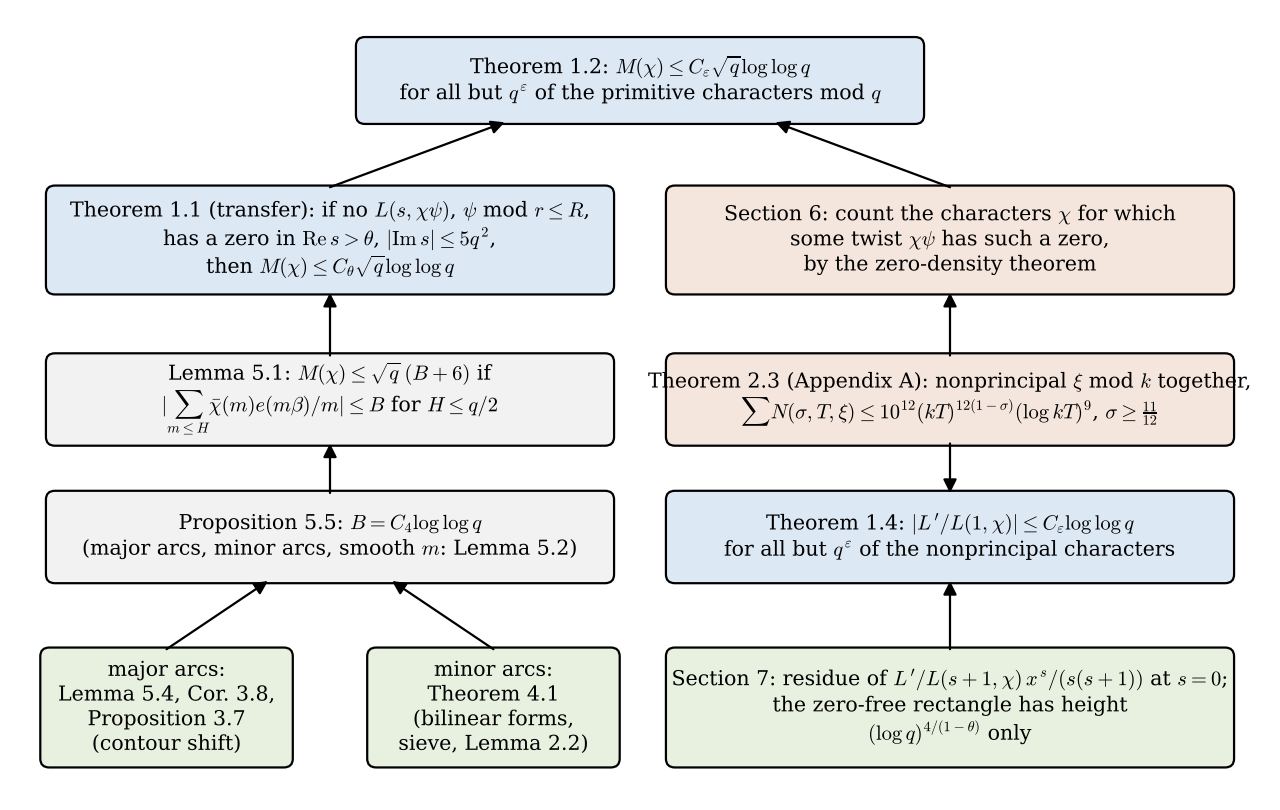
\includegraphics[width=0.96\textwidth]{figures/fig_flow.png}
\caption{The structure of the proofs. The character sum is reduced to the sums $\sum_{m\le H}\bar\chi(m)e(m\beta)/m$, which are bounded on the major arcs by the prime sums of the twists $\chi\psi$ (Proposition~\ref{prop:riesz}, Corollary~\ref{cor:prime}, Lemma~\ref{lem:major}) and on the minor arcs by Theorem~\ref{thm:mv}. The zero-density theorem bounds the number of characters for which the major-arc input fails (middle column). The zero-free half-plane of Appendix~\ref{app:halfplane} removes the exceptions and gives the Euler--Kronecker bounds of Section~\ref{sec:ek} (right column).}
\label{fig:flow}
\end{figure}

The paper is organised as follows. Section~\ref{sec:prelim} collects Chebyshev's bounds, Selberg's sieve and the zero-density theorem. Section~\ref{sec:riesz} bounds Riesz means of prime sums by a contour shift in a rectangle. Section~\ref{sec:mv} proves the bound for exponential sums with multiplicative coefficients. Section~\ref{sec:pv} proves Theorem~\ref{thm:transfer}, Section~\ref{sec:count} proves Theorem~\ref{thm:main} and Corollary~\ref{cor:halfplane}, and Section~\ref{sec:logderiv} proves Theorem~\ref{thm:logderiv}.

\section{Preliminaries}\label{sec:prelim}

Throughout, $p$ and $\ell$ denote primes, $\Lambda$ is the von Mangoldt function,
$\theta(x)=\sum_{p\le x}\log p$, $\psi(x)=\sum_{n\le x}\Lambda(n)$, $e(x)=e^{2\pi ix}$, and
$\|x\|$ is the distance from $x$ to the nearest integer. We write $\omega(n)$ for the number of
prime factors of $n$, $\Omega(n)$ for the number of prime factors counted with multiplicity, and $P(n)$
for the largest prime factor of $n\ge2$, with $P(1)=1$. The letter $\theta$ is also used for the abscissa of a zero-free rectangle; the two uses are never close to each other.

\begin{lemma}\label{lem:chebyshev}
For $x\ge1$ and integers $N\ge2$,
\begin{enumerate}
\item[(i)] $\theta(x)\le x\log4$;
\item[(ii)] $\psi(x)-\theta(x)\le2\sqrt x\log x$ and $\psi(x)\le4x$;
\item[(iii)] $\sum_{p\le N}\frac{\log p}p\le\log N+\log4$;
\item[(iv)] $\sum_{p\le N}\frac1p\le\log\log N+10$;
\item[(v)] $\sum_{n\le x}\frac{\Lambda(n)}n\le\log x+3$.
\end{enumerate}
\end{lemma}

\begin{proof}
(i) It suffices to treat integers $m\ge1$, and we use induction on $m$. The cases $m=1,2$ are
clear, and for even $m>2$ we have $\theta(m)=\theta(m-1)$. Let $m=2n+1$. The primes in
$(n+1,2n+1]$ divide $\binom{2n+1}n$, and $2\binom{2n+1}n\le2^{2n+1}$ because $\binom{2n+1}n$ and
$\binom{2n+1}{n+1}$ are equal terms of the binomial expansion of $(1+1)^{2n+1}$. Hence
$\theta(2n+1)\le\theta(n+1)+n\log4\le(2n+1)\log4$.

(ii) We have $\psi(x)-\theta(x)=\sum_{k\ge2}\theta(x^{1/k})$, where only $k\le\log x/\log2$
contribute. Each term is at most $\sqrt x\log4$ by~(i), so the sum is at most
$(\log x/\log2)\sqrt x\log4=2\sqrt x\log x$. Since $\log x\le\sqrt x$, $\psi(x)\le(\log4+2)x\le4x$.

(iii) By Legendre's formula and~(i),
\[
  N\log N\ge\log N!\ge\sum_{p\le N}\Bigl\lfloor\frac Np\Bigr\rfloor\log p
  \ge N\sum_{p\le N}\frac{\log p}p-N\log4.
\]

(iv) Let $A(u)=\sum_{p\le u}\log p/p$. Partial summation and~(iii) give
\[
  \sum_{p\le N}\frac1p=\frac{A(N)}{\log N}+\int_2^N\frac{A(u)}{u\log^2u}\,du
  \le1+\frac{\log4}{\log2}+\int_2^N\Bigl(\frac1{u\log u}+\frac{\log4}{u\log^2u}\Bigr)du,
\]
and the integral is at most $\log\log N-\log\log2+2$.

(v) The primes contribute at most $\log x+\log4$ by~(iii) applied to $N=\lfloor x\rfloor$ (for $x<2$ the sum is empty). The prime powers $p^k$ with $k\ge2$ contribute at most
$\sum_p\log p\sum_{k\ge2}p^{-k}=\sum_p\log p/(p(p-1))$. The primes $p\le7$ give $\log2/2+\log3/6+\log5/20+\log7/42<0.66$, and the primes $p\ge11$ give at most $\sum_{p\ge11}2\sqrt p/(p(p-1))\le2\sum_{n\ge11}n^{-3/2}\le2\int_{10}^\infty u^{-3/2}du<0.64$, since $\log p\le2\sqrt p$. The total is at most $\log x+\log4+1.3<\log x+3$.
\end{proof}

We use Selberg's upper bound sieve in the following form; for the method
see~\cite[Chapter~3]{HR74}, and we give the proof of the form we need.\footnote{The weights
$\lambda_d$ are those of Selberg's quadratic form, and the only feature used later is the bound
$|\lambda_d|\le1$, which makes the remainder term at most a sum of $3^{\omega(d)}|R_d|$ over
$d\le y$.}

\begin{lemma}\label{lem:selberg}
Let $a_1,\dots,a_X$ be integers, $P$ a squarefree integer, $\nu$ a multiplicative function with
$0<\nu(p)<1$ for $p\mid P$, and $y\ge1$. For $d\mid P$ put
$R_d=\#\{n\le X:d\mid a_n\}-\nu(d)X$, and for $l\mid P$ put
$g(l)=\prod_{p\mid l}\nu(p)/(1-\nu(p))$. Then
\[
  \#\{n\le X:(a_n,P)=1\}\le\frac XS+\sum_{\substack{d\mid P\\d\le y}}3^{\omega(d)}|R_d|,
  \qquad S=\sum_{\substack{l\mid P\\l\le\sqrt y}}g(l).
\]
\end{lemma}

\begin{proof}
Let $D$ be the set of divisors $d$ of $P$ with $d\le\sqrt y$, and let $(\lambda_d)_{d\in D}$ be
real numbers with $\lambda_1=1$. If $(a_n,P)=1$ then $\sum_{d\in D,\,d\mid a_n}\lambda_d=1$, and
otherwise this sum is real, so
\begin{align*}
  \#\{n:(a_n,P)=1\}&\le\sum_{n\le X}\Bigl(\sum_{\substack{d\in D\\d\mid a_n}}\lambda_d\Bigr)^2\\
  &=X\sum_{d_1,d_2\in D}\lambda_{d_1}\lambda_{d_2}\nu([d_1,d_2])
  +\sum_{d_1,d_2\in D}\lambda_{d_1}\lambda_{d_2}R_{[d_1,d_2]}.
\end{align*}
Write $Q$ for the double sum in the first term. Since $\nu$ is multiplicative and $d_1,d_2$ are
squarefree, $\nu([d_1,d_2])=\nu(d_1)\nu(d_2)/\nu((d_1,d_2))$. Let $h$ be the multiplicative
function on the divisors of $P$ with $h(p)=1/\nu(p)-1=1/g(p)$; then $1/\nu(m)=\sum_{l\mid m}h(l)$
for $m\mid P$, and
\[
  Q=\sum_{l\mid P}h(l)\Bigl(\sum_{\substack{d\in D\\l\mid d}}\lambda_d\nu(d)\Bigr)^2
  =\sum_{l\in D}\frac{y_l^2}{g(l)},\qquad y_l=\sum_{\substack{d\in D\\l\mid d}}\lambda_d\nu(d).
\]
M\"obius inversion gives $\lambda_d\nu(d)=\sum_{l\in D,\,d\mid l}\mu(l/d)y_l$, so the condition
$\lambda_1=1$ reads $\sum_{l\in D}\mu(l)y_l=1$. By Cauchy's inequality
\[
  1\le\Bigl(\sum_{l\in D}\frac{y_l^2}{g(l)}\Bigr)\Bigl(\sum_{l\in D}g(l)\Bigr)=QS,
\]
with equality for $y_l=\mu(l)g(l)/S$. We make this choice, so that $Q=1/S$. Then, writing
$l=de$,
\[
  \lambda_d=\frac{1}{\nu(d)S}\sum_{\substack{l\in D\\d\mid l}}\mu(l/d)\mu(l)g(l)
  =\frac{\mu(d)g(d)}{\nu(d)S}\sum_{\substack{e\in D,\ (e,d)=1\\de\le\sqrt y}}g(e).
\]
Since $g(d)/\nu(d)=\prod_{p\mid d}(1-\nu(p))^{-1}=\prod_{p\mid d}(1+g(p))=\sum_{f\mid d}g(f)$, we
get $|\lambda_d|\le S^{-1}\sum_{f\mid d}\sum_eg(fe)$, and the products $fe$ are distinct elements
of $D$; hence $|\lambda_d|\le1$. Finally $[d_1,d_2]\le d_1d_2\le y$, and every $d\mid P$ is the
least common multiple of at most $3^{\omega(d)}$ pairs $(d_1,d_2)$, so the second term is at most
$\sum_{d\mid P,\,d\le y}3^{\omega(d)}|R_d|$.
\end{proof}

For a Dirichlet character $\xi$ modulo $k$, real $\sigma$ and $T\ge2$ let
\[
  N(\sigma,T,\xi)=\#\{\rho=\beta+i\gamma:L(\rho,\xi)=0,\ \beta\ge\sigma,\ |\gamma|\le T\}.
\]
For $\sigma>0$ the zeros counted are those of the $L$-function of the primitive character inducing $\xi$, since the Euler factors removed in passing from that character to $\xi$ vanish only on the line $\Re s=0$. The zero-density theorem we need is the following; it is proved in Appendix~\ref{app:zd}, with the constant written out.

\begin{theorem}\label{thm:zd}
Let $c_0=10^{12}$. For every $k\ge3$, every $T\ge2$ and every $\sigma$ with $11/12\le\sigma\le1$,
\begin{equation}\label{eq:zd}
  \sum_{\substack{\xi\bmod k\\ \xi\ne\xi_0}}N(\sigma,T,\xi)\le c_0\,(kT)^{12(1-\sigma)}(\log kT)^{9},
\end{equation}
the sum running over the nonprincipal characters modulo $k$.
\end{theorem}

Theorems~12.1 and~12.2 of~\cite{Mon71} give the sum over all characters modulo $k$, principal character included, with the bounds $\ll(kT)^{3(1-\sigma)/(2-\sigma)}(\log kT)^9$ for $1/2\le\sigma\le4/5$ and $\ll(kT)^{2(1-\sigma)/\sigma}(\log kT)^{14}$ for $4/5\le\sigma\le1$, with unspecified absolute constants; these are stronger than~\eqref{eq:zd} in the exponent of $kT$. We prove the weaker form~\eqref{eq:zd} because its constant is explicit and because the proof, which follows Ingham~\cite{Ing40} and Montgomery, is short enough to be given in full.\footnote{Whether the zeros are counted in $0<\gamma\le T$ or in $|\gamma|\le T$ affects only the constant, since the zeros of $L(s,\bar\xi)$ are the conjugates of the zeros of $L(s,\xi)$ and the sum is over all characters modulo $k$.} In the proof of Theorem~\ref{thm:main} only the shape of~\eqref{eq:zd} matters, namely that the exponent of $kT$ tends to zero with $1-\sigma$.

\section{Riesz means of prime sums}\label{sec:riesz}

For an arithmetic function $a$ and $x\ge1$ put
\[
  S(a;x)=\sum_{n\le x}a(n)\Bigl(1-\frac nx\Bigr),\qquad
  S(\xi;x)=S(\xi\Lambda;x)=\sum_{n\le x}\xi(n)\Lambda(n)\Bigl(1-\frac nx\Bigr).
\]
The weight $1-n/x$ makes the Mellin kernel absolutely integrable, which keeps the contour shift
below free of truncation errors. The aim of this section is Proposition~\ref{prop:riesz}, which bounds $S(\xi;x)$ with a power saving when $L(s,\xi)$ has no zero in a rectangle of height $x^2+2$ to the left of $\Re s=1$.

\begin{lemma}\label{lem:mellin}
Let $a\colon\N\to\C$ satisfy $\sum_n|a(n)|n^{-\sigma}<\infty$ for $\sigma>1$, and let
$F(s)=\sum_na(n)n^{-s}$ for $\Re s>1$.
\begin{enumerate}
\item[(i)] For $\Re s>1$, $\displaystyle\int_1^\infty S(a;x)\,x^{-s-1}\,dx=\frac{F(s)}{s(s+1)}$.
\item[(ii)] For $x>0$, $\displaystyle S(a;x)=\frac1{2\pi}\int_{-\infty}^{\infty}
F(2+it)\,\frac{x^{2+it}}{(2+it)(3+it)}\,dt$.
\end{enumerate}
\end{lemma}

\begin{proof}
(i) For $n\ge1$, $\int_n^\infty(1-n/x)x^{-s-1}dx=n^{-s}/s-n^{-s}/(s+1)=n^{-s}/(s(s+1))$. Since
$\sum_n|a(n)|\int_n^\infty x^{-\sigma-1}dx=\sigma^{-1}\sum_n|a(n)|n^{-\sigma}<\infty$, the sum
and the integral may be exchanged.

(ii) For $y>0$ let $k(y)=\frac1{2\pi i}\int_{(2)}y^s\,\frac{ds}{s(s+1)}$. If $y\ge1$, moving the
line of integration to $\Re s=-U$, with $U>2$, picks up the residues $1$ at $s=0$ and
$-1/y$ at $s=-1$. For each fixed $U$, the horizontal integrals tend to zero as their
height tends to infinity: their lengths are fixed and the denominator is of order
the square of that height. On the new vertical line,
\[
 \int_{-\infty}^{\infty}\frac{|y^{-U+it}|}{|(-U+it)(1-U+it)|}\,dt
 \le y^{-U}\int_{-\infty}^{\infty}\frac{dt}{(U-1)^2+t^2}
 =\frac{\pi y^{-U}}{U-1}.
\]
This tends to zero for $y\ge1$, including $y=1$, so $k(y)=1-1/y$ there.
For $y<1$, shifting instead to $\Re s=U$ crosses no pole and leaves an integral
bounded by $\pi y^U/U$, which tends to zero. As
$|s(s+1)|^{-1}$ is integrable on $\Re s=2$ and $\sum_n|a(n)|n^{-2}<\infty$, summation and
integration may be exchanged, and the right side equals $\sum_na(n)k(x/n)=S(a;x)$.
\end{proof}

\begin{lemma}\label{lem:size}
Let $\chi$ be nonprincipal modulo $q$. For $\Re s=\sigma>0$, $|L(s,\chi)|\le q|s|/\sigma$.
\end{lemma}

\begin{proof}
Put $A(t)=\sum_{n\le t}\chi(n)$; then $|A(t)|\le q$, since the sum of $\chi$ over a period vanishes, and partial summation gives
$L(s,\chi)=s\int_1^\infty A(t)t^{-s-1}\,dt$ for $\sigma>0$. Hence
$|L(s,\chi)|\le q|s|\int_1^\infty t^{-\sigma-1}dt=q|s|/\sigma$.
\end{proof}

\begin{lemma}\label{lem:euler}
Let $A_0=\frac32\sum_\ell\ell^{-3/2}$. For every Dirichlet character $\chi$ the series
$E(s)=-\sum_\ell\log(1-\chi(\ell)\ell^{-s})$ is holomorphic on $\Re s>1$, $e^{E(s)}=L(s,\chi)$
there, and $|E(s)|\le A_0$ for $\Re s\ge3/2$. Moreover $|L'/L(s,\chi)|\le2$ for $\Re s\ge2$.
\end{lemma}

\begin{proof}
For $\Re s\ge1$ we have $|\chi(\ell)\ell^{-s}|\le1/2$, and $|\log(1-w)|\le\sum_k|w|^k/k
\le\frac32|w|$ for $|w|\le1/2$: indeed, the terms with $k\ge2$ have total at most
$|w|^2/(2(1-|w|))\le |w|/2$. The series therefore converges locally uniformly on $\Re s>1$
and is bounded by $A_0$ on $\Re s\ge3/2$, and the Euler product gives $e^E=L$. For $\Re s\ge2$ the derivative $E'(s)=-\sum_n\chi(n)\Lambda(n)n^{-s}$ has modulus at most $\sum_{n\ge2}\log n/n^2$, and since $\log u/u^2$ decreases for $u\ge2$ this is at most $\log2/4+\int_2^\infty\log u\,u^{-2}\,du=\log2/4+(1+\log2)/2<2$.
\end{proof}

\begin{lemma}[Borel--Carath\'eodory]\label{lem:bc}
Let $h$ be holomorphic on a neighbourhood of the disc $|z-c|\le R$ and let $0<r<R$. Then
\[
  \max_{|z-c|\le r}|h(z)-h(c)|\le\frac{2r}{R-r}\max_{|w-c|=R}\Re\bigl(h(w)-h(c)\bigr).
\]
\end{lemma}

\begin{proof}
Put $g(z)=h(c+z)-h(c)$ and $A=\max_{|w|=R}\Re g(w)$. The mean of $\Re g$ over the circle
$|w|=R$ is $\Re g(0)=0$, so $A\ge0$. If $A=0$, then $\Re g$ vanishes on the circle, hence on the
disc, and $g$ is an imaginary constant equal to $g(0)=0$. Let $A>0$. By the maximum principle
$\Re g\le A$ on $|z|\le R$, so $|2A-g|\ge A$ there and $\phi=g/(2A-g)$ is holomorphic. Since
$|g|^2-|2A-g|^2=4A(\Re g-A)\le0$, we have $|\phi|\le1$, and $\phi(0)=0$. Schwarz's lemma gives
$|\phi(z)|\le|z|/R$, and from $g=2A\phi/(1+\phi)$ we get $|g(z)|\le2A|z|/(R-|z|)$.
\end{proof}

\begin{lemma}\label{lem:logderiv}
Let $0<\delta<1/1000$, $1/2\le a\le1$, $t\in\R$, and let $\chi$ be nonprincipal modulo $q$ with
$L(s,\chi)\ne0$ for $\Re s>a+2\delta$, $|\Im s-t|\le2$. Put $K_1=(1+2A_0)/(2\delta^2)$. For
$a+8\delta\le\sigma\le2$,
\[
  \Bigl|\frac{L'}{L}(\sigma+it,\chi)\Bigr|\le K_1\log\bigl(2q(3+|t|)^2\bigr).
\]
\end{lemma}

\begin{proof}
Let $c=2+it$, $R=2-a-3\delta$, $r=2-a-6\delta$ and $\Lambda_0=\log(2q(3+|t|)^2)\ge\log18>1$.
The disc $|z-c|<2-a-2\delta$ has radius at most $3/2$, so it lies in the strip $|\Im z-t|\le2$, and on it $\Re z>a+2\delta$; hence $L(z,\chi)$ has no zero there
and has a holomorphic logarithm $h$. On $|z-c|<1/2$ both $h$ and the function $E$ of
Lemma~\ref{lem:euler} are logarithms of $L$, so they differ by a constant in $2\pi i\Z$; we
choose $h=E$ there. Then $|h(c)|\le A_0$.

If $|z-c|\le R$, then $\Re z\ge a+3\delta\ge1/2$ and $|z|\le|c|+3/2\le4+|t|$, so
Lemma~\ref{lem:size} gives $\Re h(z)=\log|L(z,\chi)|\le\log(2q(4+|t|))\le\Lambda_0$.
Lemma~\ref{lem:bc} gives, for $|z-c|\le r$,
\[
  |h(z)-h(c)|\le\frac{2r}{R-r}\bigl(\Lambda_0+A_0\bigr)\le\frac{\Lambda_0+A_0}{\delta},
\]
as $r\le3/2$ and $R-r=3\delta$. Hence $|h(z)|\le A_0+(\Lambda_0+A_0)/\delta\le(1+2A_0)\Lambda_0/\delta$
on $|z-c|\le r$. For $w=\sigma+it$ with $a+8\delta\le\sigma\le2$ we have $|w-c|=2-\sigma\le r-2\delta$,
so the circle $|z-w|=2\delta$ lies in $|z-c|\le r$, and Cauchy's estimate gives
$|L'/L(w,\chi)|=|h'(w)|\le(1+2A_0)\Lambda_0/(2\delta^2)$.
\end{proof}

\begin{lemma}\label{lem:elementary}
For $q\ge1$, $t\in\R$ and $s=\sigma+it$ with $\sigma\ge1/2$,
\[
  \log\bigl(2q(3+|t|)^2\bigr)\le10\log(q+2)(1+|t|)^{1/2},\qquad |s(s+1)|\ge\tfrac18(1+|t|)^2.
\]
\end{lemma}

\begin{proof}
We have $\log(2q)\le2\log(q+2)$, and $\log y\le2y^{1/2}$ with $3+|t|\le4(1+|t|)$ gives
$\log(3+|t|)\le4(1+|t|)^{1/2}$; the first bound follows from $\log(q+2)\ge1$. For the second,
$|s|\ge\max(\sigma,|t|)\ge(1+|t|)/4$ and $|s+1|\ge\max(\sigma+1,|t|)\ge(1+|t|)/2$.
\end{proof}

\begin{proposition}\label{prop:riesz}
Let $0<\delta<1/1000$, $1/2\le a\le1$, and put $K=90K_1+6$ with $K_1$ as in Lemma~\ref{lem:logderiv}. Let $x\ge1$ and let $\xi$ be nonprincipal modulo $k$ with $L(s,\xi)\ne0$ for $\Re s>a+2\delta$, $|\Im s|\le x^2+2$. Then
\[
  |S(\xi;x)|\le K\,x^{a+8\delta}\log(k+2).
\]
\end{proposition}

\begin{proof}
Put $\sigma_0=a+8\delta$, $T=x^2$ and
\[
  \Phi(s)=-\frac{L'}{L}(s,\xi)\,\frac{x^s}{s(s+1)}.
\]
For $\Re s>1$, $-L'/L(s,\xi)=\sum_n\xi(n)\Lambda(n)n^{-s}$, so Lemma~\ref{lem:mellin}(ii) gives
$2\pi S(\xi;x)=\int_{-\infty}^\infty\Phi(2+it)\,dt$. We split the integral at $|t|=T$.

For $|t|>T$ we use the line $\Re s=2$ as it stands: $|L'/L(2+it,\xi)|\le2$ by Lemma~\ref{lem:euler}, $|x^{2+it}|=x^2$ and $|s(s+1)|\ge(1+|t|)^2/8$ by Lemma~\ref{lem:elementary}, so
\[
  \int_{|t|>T}|\Phi(2+it)|\,dt\le2\int_T^\infty\frac{16x^2}{(1+t)^2}\,dt=\frac{32x^2}{1+T}\le32.
\]

For $|t|\le T$ we move the line of integration to $\Re s=\sigma_0$ inside the rectangle $\sigma_0\le\Re s\le2$, $|\Im s|\le T$ (Figure~\ref{fig:splane}). The function $\Phi$ is holomorphic on a neighbourhood of this rectangle, since $L(s,\xi)$ has no zero with $\Re s\ge\sigma_0>a+2\delta$ and $|\Im s|\le T+2$, and $s(s+1)\ne0$ there. By Cauchy's theorem the integral of $\Phi$ over the right side equals the integral over the left side plus the integrals over the two horizontal sides, with the appropriate orientations. On the rectangle, Lemma~\ref{lem:logderiv} applies at every point $\sigma+it$, because the hypothesis gives $L(s,\xi)\ne0$ for $\Re s>a+2\delta$ and $|\Im s-t|\le2$ when $|t|\le T$, and with Lemma~\ref{lem:elementary} it gives
\[
  |\Phi(\sigma+it)|\le80K_1\log(k+2)\,x^{\sigma}(1+|t|)^{-3/2}\qquad(\sigma_0\le\sigma\le2,\ |t|\le T).
\]
Since $\int_\R(1+|t|)^{-3/2}dt=4$, the left side contributes at most $320K_1\log(k+2)x^{\sigma_0}$. Each horizontal side has length $2-\sigma_0\le3/2$ and lies at height $T$, so it contributes at most
\[
  \tfrac32\cdot80K_1\log(k+2)\,x^2(1+T)^{-3/2}\le120K_1\log(k+2)\,x^{-1}\le120K_1\log(k+2)\,x^{\sigma_0},
\]
because $x^2(1+x^2)^{-3/2}\le x^{-1}$. Adding the three contributions and the tail, and using $\log(k+2)\ge1$ and $x^{\sigma_0}\ge1$,
\[
  2\pi|S(\xi;x)|\le(560K_1+32)\,x^{\sigma_0}\log(k+2),
\]
and $(560K_1+32)/(2\pi)\le90K_1+6$.
\end{proof}

\begin{figure}[ht]
\centering
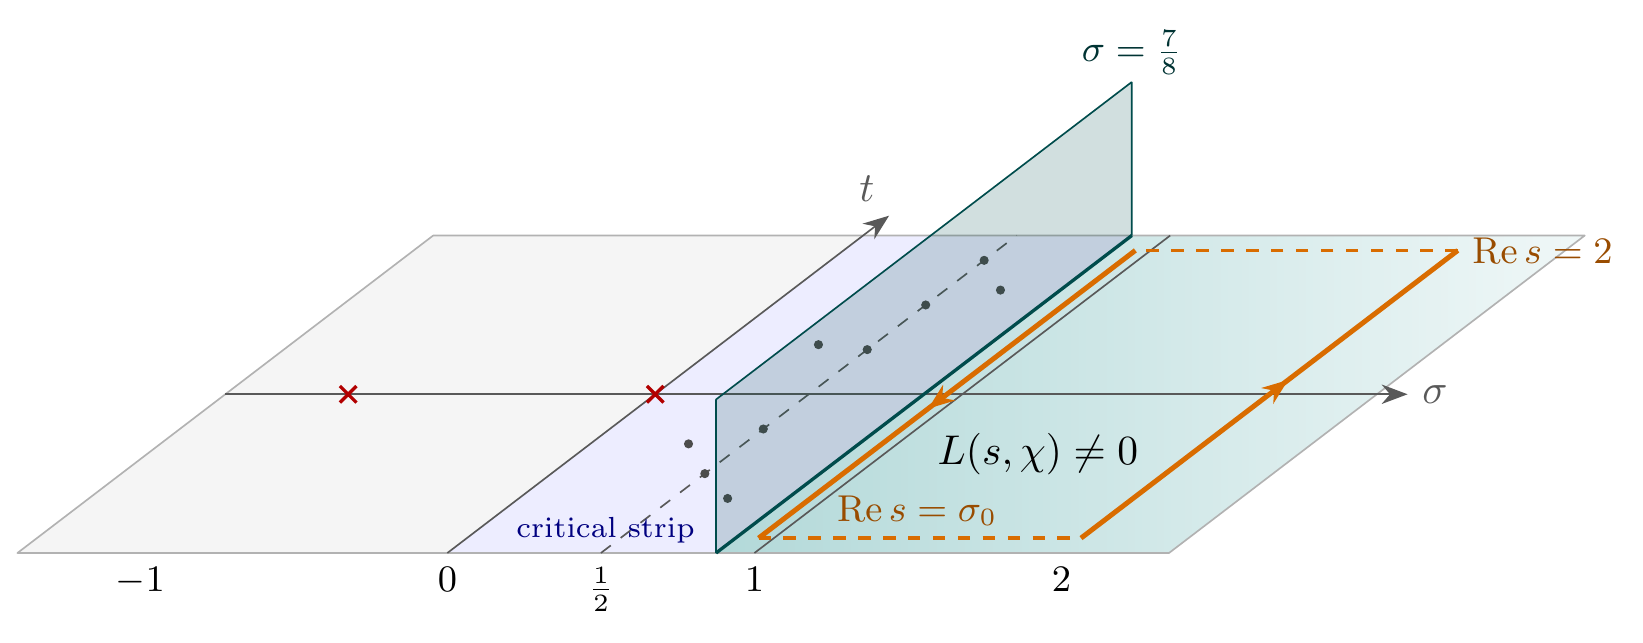
\includegraphics[width=0.8\textwidth]{figures/fig_splane.png}
\caption{The contour shift in the proof of Proposition~\ref{prop:riesz}. The integral over the line $\Re s=2$ is cut at the height $T=x^2$; the part beyond is bounded by the decay of the kernel, and the part within is moved to the line $\Re s=\sigma_0$ through the rectangle, which lies inside the region $\Re s>a+2\delta$, $|\Im s|\le x^2+2$ where $L(s,\xi)$ has no zero (dots: zeros outside that region; crosses: the poles of the kernel at $0$ and $-1$). Horizontal spacing is schematic.}
\label{fig:splane}
\end{figure}

\subsection*{Parameters}
For $1/2\le\theta<1$ we fix once and for all
\begin{equation}\label{eq:parameters}
  \delta_\theta=\min\Bigl(\frac1{2000},\frac{1-\theta}{100}\Bigr),\quad
  a_\theta=\max\Bigl(\frac12,\theta-2\delta_\theta\Bigr),\quad
  \sigma_\theta=a_\theta+8\delta_\theta,\quad
  \eta_\theta=\frac{1-\sigma_\theta}4,
\end{equation}
and we write $K_\theta$ for the constant $K$ of Proposition~\ref{prop:riesz} with $\delta=\delta_\theta$. Then $0<\delta_\theta<1/1000$, $1/2\le a_\theta\le1$ and $a_\theta+2\delta_\theta\ge\theta$, so that a character with no zero in $\Re s>\theta$, $|\Im s|\le x^2+2$ satisfies the hypothesis of Proposition~\ref{prop:riesz}. Moreover
\begin{equation}\label{eq:sigmatheta}
  \theta<\sigma_\theta<1,\qquad 1-\sigma_\theta\ge\tfrac12(1-\theta),\qquad \tfrac18(1-\theta)\le\eta_\theta\le\tfrac18.
\end{equation}
Indeed, if $a_\theta=\theta-2\delta_\theta$ then $\sigma_\theta=\theta+6\delta_\theta\le\theta+\frac6{100}(1-\theta)$, and if $a_\theta=1/2$ then $\theta<1/2+2\delta_\theta$ and $\sigma_\theta=1/2+8\delta_\theta\le1/2+8/2000$, while $1-\theta\le1/2$; in both cases $\theta<\sigma_\theta$ and $1-\sigma_\theta\ge\frac{94}{100}(1-\theta)$. The upper bound $\eta_\theta\le1/8$ follows from $\sigma_\theta\ge1/2$.

\begin{corollary}\label{cor:prime}
Let $1/2\le\theta<1$, with the parameters~\eqref{eq:parameters}, and put $C_3=8K_\theta+8/\eta_\theta$. Let $x\ge1$ and let $\xi$ be nonprincipal modulo $k$ with $L(s,\xi)\ne0$ for $\Re s>\theta$, $|\Im s|\le4x^2+2$. Then:
\begin{enumerate}
\item[(i)] $|S(\xi;y)|\le K_\theta\,y^{\sigma_\theta}\log(k+2)$ for $1\le y\le2x$;
\item[(ii)] $\bigl|\sum_{p\le x}\xi(p)\log p\bigr|\le C_3x^{1-\eta_\theta}\log(k+2)$;
\item[(iii)] for integers $2\le A\le B\le x$ and $\gamma\in\R$,
\begin{equation}\label{eq:twistedprime}
  \Bigl|\sum_{A<p\le B}\xi(p)e(p\gamma)\Bigr|\le
  2C_3\,\frac{B^{1-\eta_\theta}\log(k+2)(2+2\pi|\gamma|B)}{\log A}.
\end{equation}
\end{enumerate}
\end{corollary}

\begin{proof}
Write $\sigma=\sigma_\theta$, $\eta=\eta_\theta$ and $K=K_\theta$, so that $1+\sigma=2-4\eta$. (i) For $y\le2x$ we have $y^2+2\le4x^2+2$, so Proposition~\ref{prop:riesz} applies to $y$.

(ii) Put $T(y)=yS(\xi;y)=\sum_{n\le y}\xi(n)\Lambda(n)(y-n)$ and $h=x^{1-2\eta}$, so that $1\le h\le x$. Then
\[
  T(x+h)-T(x)=h\sum_{n\le x}\xi(n)\Lambda(n)+\sum_{x<n\le x+h}\xi(n)\Lambda(n)(x+h-n),
\]
and the last sum has at most $h+1$ terms, each of modulus at most $h\log(2x)$. With
$|T(y)|\le Ky^{1+\sigma}\log(k+2)$ for $y\le2x$, from~(i), this gives
\[
  \Bigl|\sum_{n\le x}\xi(n)\Lambda(n)\Bigr|\le\frac{2K(2x)^{1+\sigma}\log(k+2)}h+(h+1)\log(2x).
\]
Here $(2x)^{1+\sigma}/h\le4x^{2-4\eta-1+2\eta}=4x^{1-2\eta}$, so the first term is at most $8Kx^{1-\eta}\log(k+2)$. Since $\eta\le1/8$ we have $1\le x^\eta/\eta$, and $\log x=\eta^{-1}\log x^\eta\le x^\eta/\eta$, so $\log(2x)\le1+\log x\le2x^\eta/\eta$, and the second term is at most $2x^{1-2\eta}\cdot2x^{\eta}/\eta=4x^{1-\eta}/\eta$. The prime powers $p^j$ with $j\ge2$ contribute at most
$\psi(x)-\theta(x)\le2\sqrt x\log x\le2x^{1/2+\eta}/\eta\le2x^{1-\eta}/\eta$ by Lemma~\ref{lem:chebyshev}(ii), since $\eta\le1/4$. As $\log(k+2)\ge1$, (ii) follows with $C_3=8K+8/\eta$.

(iii) Let $\Pi(u)=\sum_{p\le u}\xi(p)\log p$ and $f(u)=e(u\gamma)/\log u$. Partial summation gives
\[
  \sum_{A<p\le B}\xi(p)e(p\gamma)=f(B)\Pi(B)-f(A)\Pi(A)-\int_A^B\Pi(u)f'(u)\,du,
\]
and $|f'(u)|\le2\pi|\gamma|/\log A+1/(u\log^2u)$ for $u\ge A$. By~(ii), applied at every $u\le x$, the right side is at most
$C_3B^{1-\eta}\log(k+2)\bigl(3+2\pi|\gamma|B\bigr)/\log A$, which gives~\eqref{eq:twistedprime}.
\end{proof}
\section{Exponential sums with multiplicative coefficients}\label{sec:mv}

For $M>0$ put $w_M(\theta)=M$ if $\|\theta\|<1/M$ and $w_M(\theta)=1/\|\theta\|$ otherwise;
then $0\le w_M(\theta)\le M$ and $w_M(-\theta)=w_M(\theta)$.

\begin{theorem}\label{thm:mv}
There is an absolute constant $C_1$ with the following property. Let $f$ be completely
multiplicative with $|f(n)|\le1$, let $\alpha\in\R$, and let $a,r$ be coprime integers with
$r\ge1$, $|\alpha-a/r|\le r^{-2}$ and $2\le R\le r\le N/R$. Then
\[
  \Bigl|\sum_{n\le N}f(n)e(n\alpha)\Bigr|\le C_1\Bigl(\frac N{\log N}
  +\frac{N(\log N)^2}{R^{1/4}}\Bigr).
\]
\end{theorem}

Montgomery and Vaughan~\cite[Corollary~1]{MV77} proved this for multiplicative $f$ with
$N(\log R)^{3/2}R^{-1/2}$ in place of $N(\log N)^2R^{-1/4}$. The proof below follows their
approach, a bilinear decomposition together with the spacing of the multiples of $\alpha$ and an
upper bound for prime pairs, with cruder estimates, which suffice for Theorem~\ref{thm:transfer}.

\begin{lemma}\label{lem:spacing}
Let $a,r$ be coprime with $r\ge2$ and $|\alpha-a/r|\le r^{-2}$, and let $H\ge0$ be an integer.
\begin{enumerate}
\item[(i)] $\|k\alpha\|\ge1/(2r)$ for every integer $k$ with $0<|k|\le r/2$.
\item[(ii)] $\#\{1\le h\le H:\|h\alpha\|<t\}\le(4H/r+1)(4rt+1)$ for every $t\ge0$.
\item[(iii)] For $M>0$ and every integer $K\ge0$ with $M\le2^K$,
\begin{align*}
  \sum_{h\le H}w_M(h\alpha)&\le\Bigl(\frac{4H}r+1\Bigr)(3M+4r+8rK),\\
  \sum_{h\le H}w_M(h\alpha)^2&\le\Bigl(\frac{4H}r+1\Bigr)(20rM+3M^2).
\end{align*}
\end{enumerate}
\end{lemma}

\begin{proof}
(i) Let $z$ be the integer nearest to $k\alpha$. Since $0<|k|<r$ and $(a,r)=1$, $r\nmid ka$, so
$|ka/r-z|\ge1/r$ and $\|k\alpha\|\ge1/r-|k|\,|\alpha-a/r|\ge1/(2r)$.

(ii) Let $L=\lfloor r/2\rfloor$, so $L\ge r/4$. For $k$ in a block of $L$ consecutive integers let
$y_k=k\alpha-z_k$ with $z_k$ the integer nearest to $k\alpha$. For $k\ne k'$ in the block,
$0<|k-k'|<L\le r/2$ and $y_k-y_{k'}\equiv(k-k')\alpha\pmod1$, so $|y_k-y_{k'}|\ge1/(2r)$ by~(i).
Points of $(-t,t)$ at mutual distances at least $1/(2r)$ number at most $4rt+1$, and $[1,H]$ is
covered by at most $H/L+1\le4H/r+1$ blocks.

(iii) If $\|\theta\|\ge1/M$, let $k\ge1$ be least with $\|\theta\|<2^k/M$; then $k\le K$ because
$\|\theta\|\le1/2<2^K/M$, and $\|\theta\|\ge2^{k-1}/M$, so $w_M(\theta)\le2^{1-k}M$. Hence
\[
  w_M(\theta)^j\le M^j\,[\|\theta\|<1/M]+\sum_{k=1}^K(2^{1-k}M)^j\,[\|\theta\|<2^k/M]\qquad(j=1,2).
\]
Summing over $h\le H$ with~(ii), the first sum is at most
$(4H/r+1)\bigl(4r+M+\sum_{k\le K}(8r+2^{1-k}M)\bigr)$ and the second at most
$(4H/r+1)\bigl(4rM+M^2+\sum_{k\ge1}(16rM2^{-k}+4M^24^{-k})\bigr)$.
\end{proof}

\begin{lemma}\label{lem:bilinear}
Let $\theta,\alpha\in\R$, $U>0$, and let $A,B,N$ be nonnegative integers with $B\le A+U$.
\begin{enumerate}
\item[(i)] $\bigl|\sum_{A<x\le B}e(x\theta)\bigr|\le w_U(\theta)$.
\item[(ii)] For a finite set $V$ of positive integers and $b:V\to\C$,
\[
  \sum_{A<u\le B}\Bigl|\sum_{\substack{v\in V\\uv\le N}}b(v)e(uv\alpha)\Bigr|^2\le
  \sum_{v,v'\in V}|b(v)|\,|b(v')|\,w_U\bigl((v-v')\alpha\bigr).
\]
\item[(iii)] For $M>0$ and an integer $H\ge0$,
$\sum_{1\le m,m'\le H}w_M((m-m')\alpha)\le H\bigl(M+2\sum_{h\le H}w_M(h\alpha)\bigr)$.
\end{enumerate}
\end{lemma}

\begin{proof}
(i) If $\|\theta\|<1/U$, the sum has at most $U$ terms of modulus $1$. Otherwise
$\theta\notin\Z$, the sum has modulus at most $|e((B-A)\theta)-1|/|e(\theta)-1|$, and
$|e(\theta)-1|=2|\sin\pi\theta|\ge4\|\theta\|$, so the modulus is at most $1/(2\|\theta\|)$.
(ii) Expanding the square gives $\sum_{v,v'}b(v)\overline{b(v')}\sum_ue(u(v-v')\alpha)$, where
$u$ runs over the integers of $(A,\min(B,N/v,N/v')]$, an interval of length at most $U$; apply~(i).
(iii) For fixed $m$, the term $m'=m$ is $w_M(0)=M$, and each $h=|m-m'|\in[1,H]$ arises from at
most two $m'$.
\end{proof}

\begin{lemma}\label{lem:reduction}
Let $C_5=1+4\zeta(3/2)$. For every completely multiplicative $f$ with $|f(n)|\le1$, every
$\alpha\in\R$ and every integer $N\ge1$, the sum $S=\sum_{n\le N}f(n)e(n\alpha)$ satisfies
\[
  \Bigl|S\log N-\sum_{p\le N}\log p\,f(p)\sum_{m\le N/p}f(m)e(pm\alpha)\Bigr|\le C_5N.
\]
\end{lemma}

\begin{proof}
Write $S\log N=S_1+S_2$ with
\[
  S_1=\sum_{n\le N}f(n)e(n\alpha)\log n,\qquad S_2=\sum_{n\le N}f(n)e(n\alpha)\log(N/n).
\]
Then $|S_2|\le N\log N-\log N!\le N$, since
$N^N/N!\le e^N$. In $S_1$ write $\log n=\sum_{d\mid n}\Lambda(d)$ and $n=dm$; complete
multiplicativity gives
\[
  S_1=\sum_{d\le N}\Lambda(d)f(d)\sum_{m\le N/d}f(m)e(dm\alpha).
\]
The terms with
$d$ prime form the sum in the statement, and the others have modulus at most
\[
  N\sum_p\sum_{k\ge2}\frac{\log p}{p^k}\le2N\sum_p\frac{\log p}{p^2}\le4\zeta(3/2)N,
\]
since $\log p\le2\sqrt p$.
\end{proof}

Let $G(h)=\prod_{p\mid h}p/(p-1)$.

\begin{lemma}\label{lem:pairs}
\begin{enumerate}
\item[(i)] For every integer $X\ge2$ and every even $h\ge2$,
\[
  \#\{0\le n<X:n\text{ and }n+h\text{ prime}\}\le\frac{400\,G(h)^2X}{(\log X)^2}+3X^{3/5}.
\]
\item[(ii)] $\sum_{h\le X}G(h)^4\le e^{30}X$ for every $X\ge1$.
\end{enumerate}
\end{lemma}

\begin{proof}
(i) Apply Lemma~\ref{lem:selberg} to $a_n=n(n+h)$, $0\le n<X$, with $y=X^{1/5}$,
$z=\lfloor y\rfloor$, $P$ the product of the primes $p\le z$ with $p\nmid h$, and
$\nu(d)=2^{\omega(d)}/d$. Every $p\mid P$ is odd, so $\nu(p)=2/p<1$. For $d\mid P$ the residues $n$
with $d\mid n(n+h)$ form $2^{\omega(d)}$ classes modulo $d$ (namely $n\equiv0$ or $-h\pmod p$ for
each $p\mid d$, distinct as $p\nmid h$), and each class contains between $X/d-1$ and $X/d+1$ of
the integers $0\le n<X$; hence $|R_d|\le2^{\omega(d)}$. Since the prime factors of $d$ are at
least $3$, $3^{\omega(d)}|R_d|\le6^{\omega(d)}\le d^2\le y^2$, and the error term is at most
$y^3=X^{3/5}$.

Let $\mathcal M$ be the set of $m\le\sqrt y$ whose prime factors divide $P$. Since
$\nu(p)/(1-\nu(p))=\sum_{k\ge1}\nu(p)^k$ and $\nu(m)=2^{\Omega(m)}/m$ for these $m$, $g(l)$ is the
sum of $2^{\Omega(m)}/m$ over the $m$ whose set of prime factors is that of $l$. An $m\in\mathcal M$
is counted in $g(l)$ for $l$ the product of its prime factors, and $l\le m\le\sqrt y$. Hence,
with $\tau(m)\le2^{\Omega(m)}$ the number of divisors of $m$,
\[
  S\ge\sum_{m\in\mathcal M}\frac{2^{\Omega(m)}}m\ge\sum_{m\in\mathcal M}\frac{\tau(m)}m.
\]
Let $T=\lfloor y^{1/4}\rfloor$ and let $B$ be
the set of $b\le T$ that are prime to $h$; these $b$ are odd. For $b,b'\in B$ the product $bb'$
lies in $\mathcal M$, and a given $m$ is a product $bb'$ in at most $\tau(m)$ ways, so
$S\ge\bigl(\sum_{b\in B}1/b\bigr)^2$. If $E$ is a set of primes and $p\notin E$, every $b\le T$
prime to $E$ is uniquely $p^kb'$ with $b'$ prime to $E\cup\{p\}$, so the sum of $1/b$ over the
$b\le T$ prime to $E$ is at most $p/(p-1)$ times the same sum for $E\cup\{p\}$. Adding the prime
factors of $h$ one at a time gives
\[
  \sum_{b\in B}\frac1b\ge\frac1{G(h)}\sum_{b\le T}\frac1b\ge\frac{\log(T+1)}{G(h)}.
\]
As $T+1>y^{1/4}=X^{1/20}$, we get $S\ge(\log X)^2/(400G(h)^2)$, that is,
$X/S\le400G(h)^2X/(\log X)^2$. Finally, if $n<X$ and both $n$ and $n+h$ are prime, then
$n\le z$ or $(n(n+h),P)=1$, so the count is at most $z+1+X/S+y^3\le400G(h)^2X/(\log X)^2+3X^{3/5}$.

(ii) For $t=p-1\ge1$, $(t+1)^5\le(t+31)t^4$, that is, $(p/(p-1))^4\le1+30/p$. Hence
$G(h)^4\le\sum_d30^{\omega(d)}/d$ over the squarefree $d\mid h$, and
\begin{align*}
  \sum_{h\le X}G(h)^4&\le\sum_{d\le X}\mu(d)^2\frac{30^{\omega(d)}}d\cdot\frac Xd
  \le X\prod_p\Bigl(1+\frac{30}{p^2}\Bigr)\\
  &\le X\exp\Bigl(30\sum_{n\ge2}\frac1{n^2}\Bigr)\le e^{30}X.\qedhere
\end{align*}
\end{proof}

\begin{proof}[Proof of Theorem~\ref{thm:mv}]
Let $S$ be the sum in the theorem, $L=\log N$ and $\ell=\lfloor\log_2N\rfloor$. Since
$N\ge rR\ge4$, we have $L\ge1$. If $\ell<64$, then $L<64\log2<45$ and $|S|\le N\le45N/L$. Let now
$\ell\ge64$, and put $I=\lfloor\log_2\ell\rfloor+1$ and $J=\ell+1-4I$. Then $16^I>\ell^4$, $1\le J\le\ell\le2L$,
$I\le\ell\le2L$, $2^I\le2\ell$, $N<2^{\ell+1}=2^J16^I$ and
$J^22^J\le(\ell+1)^22^{\ell+1}\ell^{-4}\le2N$. By Lemma~\ref{lem:reduction},
$|S|L\le C_5N+|T_1|+|T_2|$, where $T_1$ and $T_2$ are the parts of
$\sum_p\log p\,f(p)\sum_{m\le N/p}f(m)e(pm\alpha)$ with $p\le2^J$ and with $p>2^J$.

\emph{The small primes.} Let $0\le j<J$, $U=2^j$, $H=\lfloor N/U\rfloor$, and for $U<x\le2U$ let
$B(x)=\sum_{m\le H,\,xm\le N}f(m)e(xm\alpha)$; the inner sum for a prime $p\in(U,2U]$ is $B(p)$.
By Cauchy's inequality, Lemma~\ref{lem:bilinear}(ii), (iii) and Lemma~\ref{lem:spacing}(iii) with
$M=U$, $K=j$,
\[
  \sum_{U<p\le2U}\log p\,|B(p)|\le\bigl(U\log^2(2U)\bigr)^{1/2}Q_j^{1/2},
\]
where $Q_j=H\bigl(U+2(4H/r+1)(3U+4r+8rj)\bigr)$.
Since $HU\le N$, $UQ_j\le7NU+(8+16j)Nr+24N^2/r+(32+64j)N^2/U$, and $\log(2U)\le j+1$. Summing over
$j<J$ with $j+1\le J$, $\sum_{j<J}2^{j/2}\le3\cdot2^{J/2}$,
$\sqrt{(32+64j)2^{-j}}\le8(j+1)(3/4)^j$ and $\sum_{j\ge0}(j+1)^2(3/4)^j=112$,
\[
  |T_1|\le3\sqrt7J\sqrt{N2^J}+J^2N\sqrt{24/r}+896N+J^2\sqrt{24JNr}.
\]
Now $J^22^J\le2N$ gives $3\sqrt7J\sqrt{N2^J}\le12N$; $r\ge R\ge\sqrt R$ gives
$\sqrt{24/r}\le5R^{-1/4}$; and $r\sqrt R\le rR\le N$ gives $\sqrt{24JNr}\le5JNR^{-1/4}$. With
$J\le2L$ and $L\ge1$, $|T_1|\le908N+60L^3NR^{-1/4}$.

\emph{The large primes.} For $p>2^J$ we have $N/p<16^I$, so the $m$ in $T_2$ lie in
$(0,16^I-1]$, the union of the blocks $(16^i-1,16^{i+1}-1]$ with $0\le i<I$. Fix $i$, let
$A=16^i-1$, $U=15\cdot16^i$ and $X=\lfloor N/16^i\rfloor$, and assume $X\ge1$, the block being
empty otherwise. Only the primes $p\in(2^J,X]$ contribute, since $p\ge X+1$ and $m\ge16^i$ give
$pm>N$. Let $V$ be the set of these primes, which are odd, and
$B(m)=\sum_{p\in V,\,pm\le N}\log p\,f(p)e(pm\alpha)$. The block is
$\sum_{A<m\le A+U}f(m)B(m)$, and by Cauchy's inequality, Lemma~\ref{lem:bilinear}(ii) and
$\log p\le\lambda=\log(X+1)$, its square is at most $U\lambda^2W$, where
\[
  W=\sum_{p,p'\in V}w_U((p-p')\alpha)=|V|U+2\sum_{h=1}^Xw_U(h\alpha)\,\#\{p\in V:p+h\in V\}.
\]
The count vanishes for odd $h$, and for even $h$ Lemma~\ref{lem:pairs}(i), applied to $X+1$,
bounds it by $400G(h)^2(X+1)\lambda^{-2}+3(X+1)^{3/5}$. By Cauchy's inequality,
Lemma~\ref{lem:pairs}(ii) and Lemma~\ref{lem:spacing}(iii),
$\sum_{h\le X}G(h)^2w_U(h\alpha)\le e^{15}\sqrt XQ^{1/2}$ with $Q=(4X/r+1)(20rU+3U^2)$, and
$\sum_{h\le X}w_U(h\alpha)\le XU$. Hence $U\lambda^2W\le A_1+800e^{15}Z+A_3$, where
\[
  A_1=U^2\lambda^2X,\qquad Z=U(X+1)\sqrt XQ^{1/2},\qquad A_3=6U^2\lambda^2(X+1)^{3/5}X.
\]
Let $\kappa=\log(N+1)\ge\lambda$ and $T_i=4^i\kappa\,(N(2N)^{3/5})^{1/2}$. Since
$U^2X=225\cdot16^i(16^iX)\le225\cdot16^iN$ and $X+1\le2N$, we get $A_1\le225T_i^2$ and
$A_3\le1350T_i^2\le37^2T_i^2$. With $w=UX\le15N$, $X\le N/16^i$ and $R\le r\le N/R$,
\begin{align*}
  Z^2\le4U^2X^3Q&=320w^3X+\frac{48w^4}r+80rw^3+12Uw^3\\
  &\le\frac{320\cdot15^3N^4}{16^i}+\frac{48\cdot15^4N^4}R+\frac{80\cdot15^3N^4}R\\
  &\qquad+180\cdot15^3\cdot16^iN^3,
\end{align*}
and every coefficient is at most $40^4$, so $Z^{1/2}\le40(N2^{-i}+2NR^{-1/4}+2^iN^{3/4})$. The
block is therefore at most
\begin{align*}
  &15T_i+40\sqrt{800e^{15}}\bigl(N2^{-i}+2NR^{-1/4}+2^iN^{3/4}\bigr)+37T_i\\
  &\qquad\le K_b\bigl(N2^{-i}+NR^{-1/4}+2^iN^{3/4}+T_i\bigr),
\end{align*}
with $K_b=80\sqrt{800e^{15}}+52$. Summing over $i<I$,
\[
  |T_2|\le K_b\bigl(2N+INR^{-1/4}+2^IN^{3/4}+4^I\kappa(N(2N)^{3/5})^{1/2}\bigr).
\]
Here $I\le2L^3$; $2^I\le4L\le16N^{1/4}$; $4^I\le16L^2$ and $\kappa\le2L$; and
$\log x\le15x^{1/15}$ gives $L^3(N(2N)^{3/5})^{1/2}\le2\cdot15^3N$. Hence
$|T_2|\le K_b(216018N+2L^3NR^{-1/4})$.

Altogether $|S|L\le(C_5+908+216018K_b)N+(60+2K_b)L^3NR^{-1/4}$, and dividing by $L$ gives the
theorem with $C_1=45+C_5+908+216018K_b+60+2K_b$.
\end{proof}


\section{Proof of Theorem~\ref{thm:transfer}}\label{sec:pv}

In this section $\chi$ is a primitive character modulo $q\ge3$.

\begin{lemma}\label{lem:polya}
Let $B\ge0$ be such that $\bigl|\sum_{m\le H}\bar\chi(m)e(m\beta)/m\bigr|\le B$ for every integer
$H\le q/2$ and every $\beta\in\R$. Then $\bigl|\sum_{n\le x}\chi(n)\bigr|\le\sqrt q\,(B+6)$ for
every $x\ge0$.
\end{lemma}

\begin{proof}
We may take $x=T$ to be an integer. Let $\tau=\sum_{a\bmod q}\bar\chi(a)e(a/q)$. Since
$\bar\chi$ is primitive, $\sum_a\bar\chi(a)e(an/q)=\chi(n)\tau$ for every $n$, and summing the
squares of the moduli of these identities over $n\bmod q$ gives $q\varphi(q)=|\tau|^2\varphi(q)$,
so $|\tau|=\sqrt q$. Summing over $1\le n\le T$,
\[
  \tau\sum_{n\le T}\chi(n)=\sum_{0<|a|\le q/2}\bar\chi(a)\,
  \frac{e(aT/q)-1}{1-e(-a/q)},
\]
where $a$ runs over the integers with $-q/2<a\le q/2$, $a\ne0$. For $0<|\vartheta|\le1/2$ put
$r(\vartheta)=(1-e(-\vartheta))^{-1}-(2\pi i\vartheta)^{-1}$; then $|1-e(-\vartheta)|=2|\sin\pi\vartheta|\ge4|\vartheta|$.
If $2\pi|\vartheta|\le1$, then $|e(-\vartheta)-1+2\pi i\vartheta|\le(2\pi\vartheta)^2$ and
$|r(\vartheta)|\le(2\pi\vartheta)^2/(4|\vartheta|\cdot2\pi|\vartheta|)<3$; otherwise
$|r(\vartheta)|\le1/(4|\vartheta|)+1/(2\pi|\vartheta|)<3$. The terms with $r(a/q)$ contribute at most
$6q$. Writing $a=\pm m$ with $1\le m\le q/2$, the remaining terms are $q/(2\pi i)$ times a
combination, with coefficients of modulus at most $1$, of four sums
$\sum_{m\le H}\bar\chi(m)e(m\beta)/m$ with $H\le q/2$, so they contribute at most $2qB/\pi$.
Dividing by $|\tau|$ gives the claim.
\end{proof}

\begin{lemma}\label{lem:smooth}
For $Y\ge2$ and $H\ge1$,
\[
  \sum_{\substack{n\le H\\P(n)\le Y}}\frac1n\le e^{11}\log Y.
\]
\end{lemma}

\begin{proof}
The sum is at most $\prod_{p\le Y}(1-1/p)^{-1}\le\exp\bigl(\sum_{p\le Y}\frac1{p-1}\bigr)$, and
$\sum_p\bigl(\frac1{p-1}-\frac1p\bigr)\le1$; apply Lemma~\ref{lem:chebyshev}(iv).
\end{proof}

\begin{lemma}\label{lem:nonprincipal}
Let $0<r<q$ and let $\psi$ be a character modulo $r$. Then the character $\chi\psi$ modulo $qr$ is nonprincipal. Moreover, if $\chi_1,\chi_2$ are primitive characters modulo $q$ with $\chi_1\psi=\chi_2\psi$, then $\chi_1=\chi_2$.
\end{lemma}

\begin{proof}
Suppose $\chi\psi$ is principal, so that $\chi(n)=\bar\psi(n)$ for every
$n$ prime to $qr$. Let $d=(q,r)$ and let $n$ be prime to $q$ with $n\equiv1\pmod d$. By the
Chinese remainder theorem there is $n'$ prime to $qr$ with $n'\equiv n\pmod q$ and
$n'\equiv1\pmod r$, and then $\chi(n)=\chi(n')=\bar\psi(n')=1$. So $\chi$ is trivial on the
units congruent to $1$ modulo $d$, and is induced by a character modulo $d\le r<q$, which
contradicts primitivity. For the second claim, $\chi_1(n)=\chi_2(n)$ for every $n$ prime to $qr$, and for $n$ prime to $q$ there is, again by the Chinese remainder theorem, an $n'$ prime to $qr$ with $n'\equiv n\pmod q$, so that $\chi_1(n)=\chi_1(n')=\chi_2(n')=\chi_2(n)$.
\end{proof}

\begin{lemma}\label{lem:major}
Let $1/2\le\theta<1$, with the parameters~\eqref{eq:parameters} and the constant $C_3$ of Corollary~\ref{cor:prime}, and put $C_2=2C_3/\eta_\theta$. Let $0<r<q$, $b\in\Z$, $\beta\in\R$, let $Y\ge\max(2,r)$ and $t\ge1$ be integers, and suppose that $L(s,\chi\psi)\ne0$ for $\Re s>\theta$, $|\Im s|\le4t^2+2$ for every character $\psi$ modulo $r$. Then
\[
  \Bigl|\sum_{\substack{n\le t\\P(n)>Y}}\chi(n)e\Bigl(n\Bigl(\frac br+\beta\Bigr)\Bigr)\Bigr|
  \le C_2\,\frac{r\log(qr+2)\,(2+2\pi|\beta|t)\,t}{Y^{\eta_\theta}\log Y}.
\]
\end{lemma}

\begin{proof}
Write $\eta=\eta_\theta$. Every $n\le t$ with $P(n)>Y$ is uniquely $n=pm$ with $p=P(n)$ prime, $Y<p\le t/m$ and
$P(m)\le p$, and then $m\le t/Y$. For such $p$ we have $p>r$, so $p\nmid r$, and on the units
modulo $r$ the function $u\mapsto e(umb/r)$ equals $\sum_\psi c_\psi\psi(u)$, the sum over the
characters $\psi$ modulo $r$, with $|c_\psi|\le1$. By Lemma~\ref{lem:nonprincipal} each $\chi\psi$ is nonprincipal modulo $qr$, and by hypothesis it satisfies the condition of Corollary~\ref{cor:prime} with $x=t$. Applying~\eqref{eq:twistedprime} to $\xi=\chi\psi$ with $\gamma=m\beta$,
$A=\max(Y,P(m)-1)$ and $B=\lfloor t/m\rfloor\le t$ (the inner sum is empty if $A\ge B$) gives
\[
  \Bigl|\sum_{\substack{n\le t\\P(n)>Y}}\chi(n)e\Bigl(n\Bigl(\frac br+\beta\Bigr)\Bigr)\Bigr|
  \le2C_3r\,\frac{\log(qr+2)(2+2\pi|\beta|t)}{\log Y}\sum_{m\le t/Y}\Bigl(\frac tm\Bigr)^{1-\eta},
\]
and $\sum_{m\le M}m^{-1+\eta}\le\int_0^Mu^{\eta-1}du=M^\eta/\eta$, so the last sum is at most $t/(\eta Y^\eta)$.
\end{proof}

\begin{proposition}\label{prop:hsum}
Let $1/2\le\theta<1$, with the parameters~\eqref{eq:parameters}, the constant $C_1$ of Theorem~\ref{thm:mv} and the constant $C_2$ of Lemma~\ref{lem:major}, and put $A_\theta=\lceil36/\eta_\theta\rceil$ and $C_4=1+5C_1+C_2+4e^{11}A_\theta$. Suppose that $\log q\ge200$, put $M=\lceil\log q\rceil$ and $R=M^{16}$, and suppose that~\eqref{eq:hyp} holds for every $r\le R$ and every character $\psi$ modulo $r$. Then
$\bigl|\sum_{m\le H}\chi(m)e(m\beta)/m\bigr|\le C_4\log\log q$ for every integer $H\le q$ and
every $\beta\in\R$.
\end{proposition}

\begin{proof}
Let $L=\log q$, $\eta=\eta_\theta$, $A=A_\theta$ and $Y=M^{A}$. Since
$e^{L/16}\ge(L/16)^4/24>L+1\ge M$, we have $2\le R<q$, and $R\le Y$ since $A\ge288$. Split the sum according to
$P(m)\le Y$ or $P(m)>Y$. By Lemma~\ref{lem:smooth} the first part is at most $e^{11}\log Y$. For
the second put $A(t)=\sum_{n\le t,\,P(n)>Y}\chi(n)e(n\beta)$ and $w(t)=1/t-1/(t+1)$. Partial
summation and $|A(H)|\le H$ give
\[
  \Bigl|\sum_{\substack{m\le H\\P(m)>Y}}\frac{\chi(m)e(m\beta)}m\Bigr|\le1+\sum_{1\le t<H}|A(t)|\,w(t).
\]
If $t\le Y$, then $A(t)=0$. Let $t>Y$ and $Q=\lfloor t/R\rfloor\ge1$. By Dirichlet's theorem
there are coprime $a,r$ with $1\le r\le Q$ and $|\beta-a/r|\le1/(r(Q+1))$; then
$|\beta-a/r|\,t\le R$ (Figure~\ref{fig:arcs}). If $r\le R$, then $r<q$, and $4t^2+2\le4q^2+2\le5q^2$ because $t<H\le q$ and $q\ge3$, so~\eqref{eq:hyp} gives the hypothesis of Lemma~\ref{lem:major} for this $r$; that lemma with $b=a$ gives $|A(t)|\le C_2kt$, where
\[
  k=\frac{R\log(qR+2)(2+2\pi R)}{Y^{\eta}\log Y}.
\]
If $r>R$, then $R\le r\le t/R$ and $|\beta-a/r|\le r^{-2}$, so Theorem~\ref{thm:mv} for $f=\chi$
bounds the full sum $\sum_{n\le t}\chi(n)e(n\beta)$, and since $\log t\le L$, removing the
$\Psi(t)=\#\{n\le t:P(n)\le Y\}$ smooth terms gives
\[
  |A(t)|\le C_1\Bigl(\frac t{\log t}+t\rho\Bigr)+\Psi(t),\qquad
  \rho=\frac{L^2}{R^{1/4}}=\frac{L^2}{M^4}.
\]
Since $tw(t)\le1/t$ and $w(t)\le1/t^2$,
\[
  \sum_{1\le t<H}|A(t)|\,w(t)\le C_1\sum_{2\le t\le H}\frac1{t\log t}
  +(C_1\rho+C_2k)\sum_{t\le H}\frac1t+\sum_{1\le t<H}\Psi(t)w(t).
\]
The first sum is at most $3+\log L$, the second at most $1+L$, and by partial summation the third
is at most $\sum_{n\le H,\,P(n)\le Y}1/n\le e^{11}\log Y$. Finally $L\le M\le2L$ gives
$\rho(1+L)\le2/M\le1$; $\log(qR+2)\le18M$, $2+2\pi R\le8M^{16}$, $Y^{\eta}=M^{A\eta}\ge M^{36}$ and
$\log Y=A\log M\ge\log M$ give $k(1+L)\le288M^{34}/(M^{36}\log M)\le1$; and
$\log Y=A\log M\le2A\log L$, since $\log M\le\log2+\log L\le2\log L$. Collecting terms, the sum is at most
$1+4C_1+C_2+(C_1+4e^{11}A)\log L\le(1+5C_1+C_2+4e^{11}A)\log L$, as $\log L\ge1$.
\end{proof}

\begin{figure}[ht]
\centering
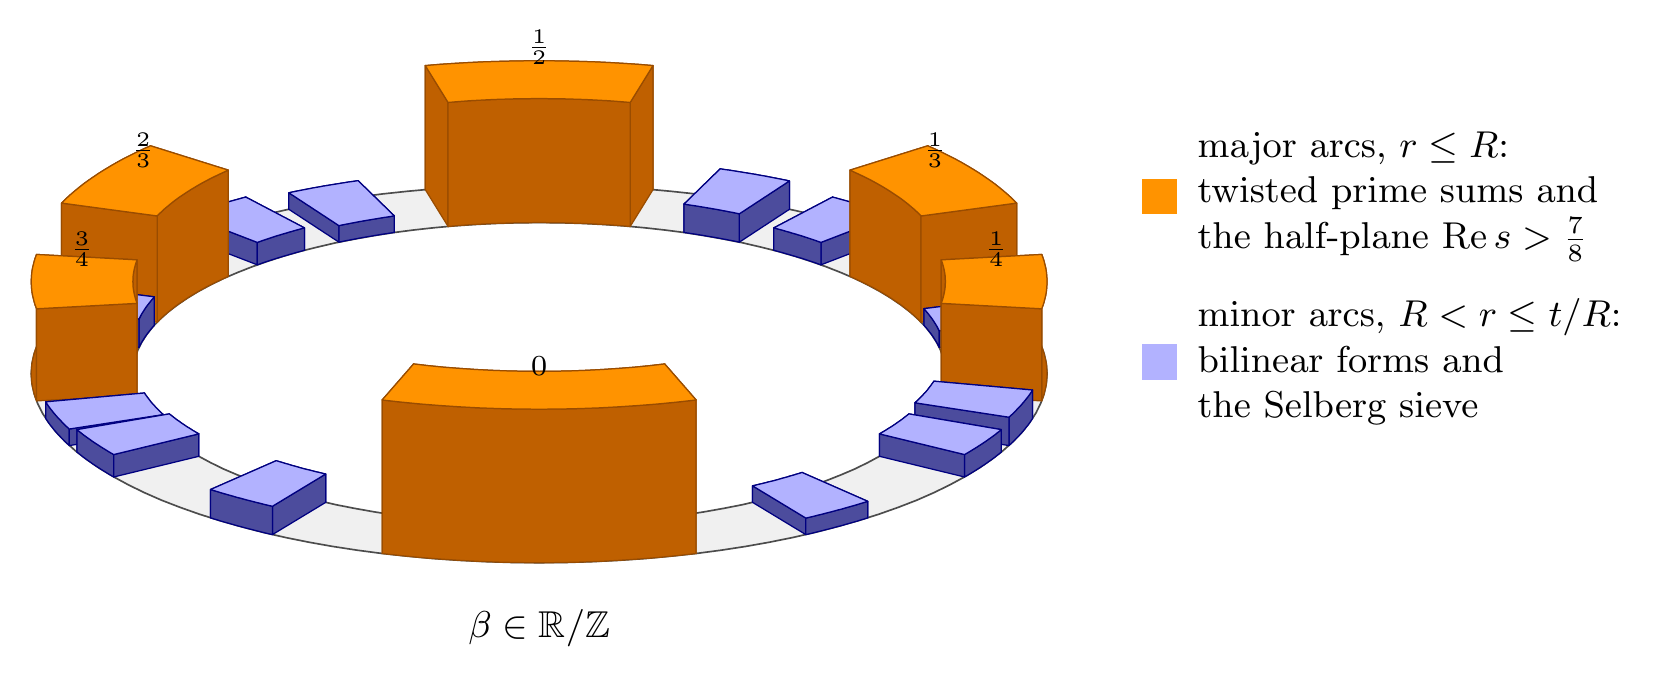
\includegraphics[width=0.96\textwidth]{figures/fig_arcs.png}
\caption{The dissection of $\mathbb R/\mathbb Z$ in the proof of
Proposition~\ref{prop:hsum}, drawn for $R=4$. Near a fraction $a/r$ with $r\le R$ (major arcs)
the sum $A(t)$ is controlled by the twisted prime sums of Corollary~\ref{cor:prime}; elsewhere
(minor arcs) by Theorem~\ref{thm:mv}. The heights only indicate that the major arcs carry the
large values.}
\label{fig:arcs}
\end{figure}

\begin{proof}[Proof of Theorem~\ref{thm:transfer}]
Put $C_\theta=\max(C_4+6,\,207/\log\log3)$ with $C_4$ as in Proposition~\ref{prop:hsum}. If $\log q<200$, then every sum $\sum_{m\le H}\bar\chi(m)e(m\beta)/m$ with $H\le q$ has modulus at
most $1+\log q<201$, and Lemma~\ref{lem:polya} gives
\[
  \Bigl|\sum_{n\le x}\chi(n)\Bigr|\le207\sqrt q\le\frac{207}{\log\log3}\sqrt q\log\log q
\]
without any hypothesis. Let $\log q\ge200$. The character $\bar\chi$ is primitive modulo $q$, and it satisfies~\eqref{eq:hyp} for every $r\le R$ and $\psi$ modulo $r$: the zeros of $L(s,\bar\chi\psi)$ are the complex conjugates of the zeros of $L(s,\chi\bar\psi)$, $\bar\psi$ is again a character modulo $r$, and the rectangle in~\eqref{eq:hyp} is symmetric about the real axis. Hence Proposition~\ref{prop:hsum} applies to $\bar\chi$, and
Lemma~\ref{lem:polya} gives
\[
  \Bigl|\sum_{n\le x}\chi(n)\Bigr|\le\sqrt q\,(C_4\log\log q+6)\le(C_4+6)\sqrt q\log\log q.\qedhere
\]
\end{proof}

\section{The exceptional characters}\label{sec:count}

\begin{proof}[Proof of Theorem~\ref{thm:main}]
It suffices to treat $0<\varepsilon\le1$, since for larger $\varepsilon$ the statement is weaker. Put $\theta=1-\varepsilon/48$, so that $47/48\le\theta<1$, and let $C_\theta$ be the constant of Theorem~\ref{thm:transfer}. Let $q$ satisfy $\log q\ge200$, put $L=\log q$, $M=\lceil L\rceil$, $R=M^{16}$, and let $E_q$ be the set of primitive characters $\chi$ modulo $q$ for which~\eqref{eq:hyp} fails for some $r\le R$ and some $\psi$ modulo $r$. By Theorem~\ref{thm:transfer}, every primitive $\chi\notin E_q$ has $M(\chi)\le C_\theta\sqrt q\log\log q$, so it remains to bound $|E_q|$.

For $\chi\in E_q$ choose $r\le R$, $\psi$ modulo $r$ and a zero $\rho$ of $L(s,\chi\psi)$ with $\Re\rho>\theta$ and $|\Im\rho|\le5q^2$. The character $\chi\psi$ is a character modulo $qr$, and $\rho$ is counted in $N(\theta,5q^2,\chi\psi)$. For fixed $r$ and $\psi$ the map $\chi\mapsto\chi\psi$ is injective by Lemma~\ref{lem:nonprincipal}, so each term $N(\theta,5q^2,\xi)$, $\xi$ modulo $qr$, is charged by at most one $\chi$ for each pair $(r,\psi)$. Each $\chi\psi$ is nonprincipal by the same lemma. Hence, by Theorem~\ref{thm:zd} with $k=qr\ge3$ and $T=5q^2$, and since $\theta\ge11/12$,
\begin{align*}
  |E_q|&\le\sum_{r\le R}\sum_{\psi\bmod r}\sum_{\substack{\xi\bmod qr\\ \xi\ne\xi_0}}N(\theta,5q^2,\xi)
  \le c_0\sum_{r\le R}\varphi(r)\,(5q^3r)^{12(1-\theta)}\bigl(\log(5q^3r)\bigr)^{9}\\
  &\le c_0R^2(5q^3R)^{\varepsilon/4}\bigl(\log(5q^3R)\bigr)^{9}.
\end{align*}
Now $M\le L+1\le2L$, so $R\le2^{16}L^{16}$ and $(5R)^{1/4}\le(5\cdot2^{16})^{1/4}L^4\le2^5L^4$; and $\log(5q^3R)\le\log(5\cdot2^{16})+3L+16\log(2L)\le20L$, since $L\ge200$. Therefore
\begin{equation}\label{eq:count}
  |E_q|\le c_0\,2^{37}\,20^{9}\,L^{45}\,q^{3\varepsilon/4}.
\end{equation}
Since $(\log q)^{45}q^{-\varepsilon/4}\to0$ as $q\to\infty$, there is $q_0=q_0(\varepsilon)\ge e^{200}$ such that $c_0\,2^{37}\,20^{9}(\log q)^{45}\le q^{\varepsilon/4}$ for $q\ge q_0$, and then $|E_q|\le q^{\varepsilon}$.

For $3\le q<q_0$ no character is exceptional: every sum $\sum_{m\le H}\bar\chi(m)e(m\beta)/m$ with $H\le q$ has modulus at most $1+\log q$, so Lemma~\ref{lem:polya} gives $M(\chi)\le(7+\log q_0)\sqrt q\le\bigl((7+\log q_0)/\log\log3\bigr)\sqrt q\log\log q$. The theorem holds with $C_\varepsilon=\max\bigl(C_\theta,(7+\log q_0)/\log\log3\bigr)$.
\end{proof}

The bound~\eqref{eq:count} is where the exponent $\varepsilon$ comes from: the zero-density theorem gives a power $q^{36(1-\theta)}$ of the modulus, times a power of $\log q$, and $\theta$ is chosen so that $36(1-\theta)=3\varepsilon/4$. Any zero-density theorem of the shape~\eqref{eq:zd}, with $12(1-\sigma)$ replaced by $c(1-\sigma)$ for an absolute $c$, gives the same conclusion with $\theta=1-\varepsilon/(4c)$; with the exponents of Montgomery's Theorem~12.2 one may take $\theta=1-\varepsilon/8$.

\begin{proof}[Proof of Corollary~\ref{cor:halfplane}]
Let $\chi$ be primitive modulo $q\ge3$, $r\le R<q$ and $\psi$ a character modulo $r$. By Lemma~\ref{lem:nonprincipal} the character $\chi\psi$ is nonprincipal, so by hypothesis $L(s,\chi\psi)\ne0$ for $\Re s>\theta$, and in particular~\eqref{eq:hyp} holds. Theorem~\ref{thm:transfer} gives the claim.
\end{proof}

\section{The logarithmic derivative at $s=1$}\label{sec:logderiv}

In this section $\chi$ is a nonprincipal character modulo $q\ge3$, not necessarily primitive.

\begin{proposition}\label{prop:logderiv}
Let $1/2\le\theta<1$, with the parameters~\eqref{eq:parameters}, let $K_1$ be the constant of Lemma~\ref{lem:logderiv} with $\delta=\delta_\theta$, and put
\[
  T_1=\bigl(\log(q+2)\bigr)^{4/(1-\theta)}+2,\qquad
  C_5=\frac6{1-\sigma_\theta}+429K_1\Bigl(1+\frac1{1-\sigma_\theta}\Bigr)+99.
\]
If $L(s,\chi)\ne0$ for $\Re s>\theta$, $|\Im s|\le T_1$, then $|L'/L(1,\chi)|\le C_5\log\log q$.
\end{proposition}

\begin{proof}
Write $\sigma=\sigma_\theta$, $a=a_\theta$, $\delta=\delta_\theta$, and put
\[
  x=\bigl(\log(q+2)\bigr)^{1/(1-\sigma)},\qquad T_0=x^2,
\]
so that $x>1$, $x^{1-\sigma}=\log(q+2)$, and $T_0+2\le T_1$ by~\eqref{eq:sigmatheta}. Note that $L(1,\chi)\ne0$ by hypothesis, since $\Re1>\theta$.

Let $a(n)=\chi(n)\Lambda(n)/n$ and $F(x)=S(a;x)=\sum_{n\le x}\chi(n)\Lambda(n)n^{-1}(1-n/x)$. The Dirichlet series of $a$ is $-L'/L(s+1,\chi)$, so Lemma~\ref{lem:mellin}(ii) gives $2\pi F(x)=\int_{-\infty}^\infty\Phi(2+it)\,dt$ with
\[
  \Phi(s)=-\frac{L'}{L}(s+1,\chi)\,\frac{x^s}{s(s+1)}.
\]
For $|t|>T_0$ Lemmas~\ref{lem:euler} and~\ref{lem:elementary} give $|\Phi(2+it)|\le16x^2(1+|t|)^{-2}$, so this part of the integral has modulus at most $32x^2/(1+T_0)\le32$.

Consider the rectangle $\sigma-1\le\Re s\le2$, $|\Im s|\le T_0$. On a neighbourhood of it the function $-L'/L(s+1,\chi)$ is holomorphic except for a simple pole at $s=0$ with residue $1$ (the pole of $L(s+1,\chi)$ is excluded since $\chi$ is nonprincipal): indeed $\Re(s+1)\ge\sigma>\theta$ by~\eqref{eq:sigmatheta} and $|\Im(s+1)|\le T_0<T_1$, so $L(s+1,\chi)\ne0$ there except at $s=0$, where $L(1,\chi)\ne0$ as well, and the pole of $-L'/L(s+1,\chi)$ at $s=0$ is the pole of the kernel $1/(s(s+1))$. The pole of the kernel at $s=-1$ lies outside the rectangle, since $\sigma-1>-1/2$. Thus $\Phi$ has in the rectangle exactly one pole, a simple pole at $s=0$ with residue $-L'/L(1,\chi)$. By the residue theorem the integral of $\Phi$ over the right side of the rectangle equals $-2\pi\,L'/L(1,\chi)$ plus the integral over the left side plus the integrals over the two horizontal sides, with the appropriate orientations. Consequently
\begin{equation}\label{eq:residue}
  2\pi\Bigl|\frac{L'}{L}(1,\chi)\Bigr|\le2\pi|F(x)|+32+I_{\mathrm{left}}+I_{\mathrm{top}}+I_{\mathrm{bottom}},
\end{equation}
where the three $I$ are the moduli of the integrals of $\Phi$ over the left and horizontal sides.

By Lemma~\ref{lem:chebyshev}(v), $|F(x)|\le\sum_{n\le x}\Lambda(n)/n\le\log x+3$.

On the left side $s=\sigma-1+it$ with $|t|\le T_0$. Lemma~\ref{lem:logderiv} applies to $L'/L(\sigma+it,\chi)$, since $a+8\delta=\sigma\le2$ and the hypothesis gives $L(s,\chi)\ne0$ for $\Re s>a+2\delta$ (as $a+2\delta\ge\theta$) and $|\Im s-t|\le2$ (as $T_0+2\le T_1$); with Lemma~\ref{lem:elementary} it gives $|L'/L(\sigma+it,\chi)|\le10K_1\log(q+2)(1+|t|)^{1/2}$. Moreover $|s|\ge\max(1-\sigma,|t|)\ge(1-\sigma)(1+|t|)/2$ and $|s+1|=|\sigma+it|\ge\max(1/2,|t|)\ge(1+|t|)/3$, so $|s(s+1)|\ge(1-\sigma)(1+|t|)^2/6$. Hence
\[
  I_{\mathrm{left}}\le\int_{-\infty}^\infty\frac{60K_1\log(q+2)\,x^{\sigma-1}}{(1-\sigma)(1+|t|)^{3/2}}\,dt=\frac{240K_1}{1-\sigma},
\]
by the choice of $x$.

On the horizontal sides $s=\sigma'\pm iT_0$ with $\sigma-1\le\sigma'\le2$, and $T_0\ge1$. For $\sigma'\le1$ Lemmas~\ref{lem:logderiv} and~\ref{lem:elementary} give $|L'/L(s+1,\chi)|\le10K_1\log(q+2)(1+T_0)^{1/2}$, and for $\sigma'>1$ the same bound holds by Lemma~\ref{lem:euler}, since $K_1\ge1$. Also $|x^s|\le x^2$ and $|s(s+1)|\ge T_0^2\ge(1+T_0)^2/4$. Each horizontal side has length at most $3$, so
\[
  I_{\mathrm{top}},\ I_{\mathrm{bottom}}\le3\cdot40K_1\log(q+2)\,x^2(1+T_0)^{-3/2}\le120K_1\log(q+2)\,x^{-1}=120K_1x^{-\sigma}\le120K_1.
\]

Inserting these bounds in~\eqref{eq:residue} and dividing by $2\pi$,
\[
  \Bigl|\frac{L'}{L}(1,\chi)\Bigr|\le\log x+3+6+\frac{39K_1}{1-\sigma}+39K_1
  =\frac{\log\log(q+2)}{1-\sigma}+39K_1\Bigl(1+\frac1{1-\sigma}\Bigr)+9.
\]
Finally $\log\log(q+2)\le6\log\log q$ for $q\ge3$, since the ratio of the two sides decreases in $q$ and is below $5.1$ at $q=3$, and $1\le11\log\log q$ since $\log\log3>1/11$. This gives the constant $C_5$.
\end{proof}

\begin{proof}[Proof of Theorem~\ref{thm:logderiv}]
As before let $0<\varepsilon\le1$, $\theta=1-\varepsilon/48$, and let $C_5$ and $T_1=(\log(q+2))^{192/\varepsilon}+2$ be as in Proposition~\ref{prop:logderiv}. Let $E'_q$ be the set of nonprincipal characters $\chi$ modulo $q$ for which $L(s,\chi)$ has a zero with $\Re s>\theta$ and $|\Im s|\le T_1$. By Proposition~\ref{prop:logderiv} every nonprincipal $\chi\notin E'_q$ satisfies $|L'/L(1,\chi)|\le C_5\log\log q$, and by Theorem~\ref{thm:zd}, as $E'_q$ contains only nonprincipal characters and $\theta\ge11/12$,
\[
  |E'_q|\le\sum_{\substack{\xi\bmod q\\ \xi\ne\xi_0}}N(\theta,T_1,\xi)\le c_0(qT_1)^{\varepsilon/4}(\log qT_1)^{9}.
\]
Here $T_1\le2(\log(q+2))^{192/\varepsilon}$, so $T_1^{\varepsilon/4}\le2(\log(q+2))^{48}$, and $\log(qT_1)\le\log q+1+192\varepsilon^{-1}\log\log(q+2)$. Hence $|E'_q|\le q^{\varepsilon/4}P_\varepsilon(\log q)$ for a polynomial $P_\varepsilon$, and there is $q_1=q_1(\varepsilon)$ with $|E'_q|\le q^{\varepsilon}$ for $q\ge q_1$. For $3\le q<q_1$ there are finitely many nonprincipal characters, each with $L(1,\chi)\ne0$ by Dirichlet's theorem~\cite[Chapter~4]{Dav80}, so $|L'/L(1,\chi)|/\log\log q$ is bounded on them by a constant $C'$ depending on $\varepsilon$; no character is exceptional there. The theorem holds with $C_\varepsilon=\max(C_5,C')$.
\end{proof}

\section{Euler--Kronecker constants of cyclotomic fields}\label{sec:ek}

For $m\ge3$ let $K_m=\mathbb Q(\zeta_m)$ and write the Laurent expansion of its Dedekind zeta function at $s=1$ as $\zeta_{K_m}(s)=c_{-1}/(s-1)+c_0+O(s-1)$. The Euler--Kronecker constant of $K_m$ is $\gamma_m=c_0/c_{-1}$~\cite{Iha06}, so that
\begin{equation}\label{eq:ekdef}
  -\frac{\zeta_{K_m}'}{\zeta_{K_m}}(s)=\frac1{s-1}-\gamma_m+O(s-1)\qquad(s\to1).
\end{equation}
Ihara proved, under the generalised Riemann hypothesis, that $\gamma_q\le(2+o(1))\log q$ for primes $q$, and conjectured bounds of the same order on both sides; Ford, Luca and Moree showed that the lower half of that conjecture fails if the prime $k$-tuples and Elliott--Halberstam conjectures hold~\cite{Iha06,FLM14}. The zero-free half-plane of Appendix~\ref{app:halfplane} gives an upper bound of the order $\log m$ with no hypothesis.

\begin{theorem}[Theorem~\ref{thm:ekintro}]\label{thm:ek}
There is an absolute constant $C$ such that
\[
  \gamma_m\le12\log m+36\log\log m+C\qquad\text{for every }m\ge3,
\]
and
\[
  \gamma_q\ge-C\log q\log\log q\qquad\text{for every prime }q\ge5.
\]
\end{theorem}

Throughout this section $\theta=11/12$, $\chi_0$ is the principal character modulo $m$, and for a character $\chi$ modulo $m$ we write $\chi^*$ for the primitive character that induces it and $\psi(x,\chi)=\sum_{n\le x}\chi(n)\Lambda(n)$. The constants $C_1,C_2,\dots$ are absolute.

\begin{lemma}\label{lem:ekpsi}
For $m\ge3$ and $x\ge2$ put $E_m(x)=\sum_{\chi\bmod m}\psi(x,\chi)-x$. Then $|E_m(x)|\le C_1\varphi(m)x^{\theta}\log^2(mx)$.
\end{lemma}

\begin{proof}
Let $\chi^*$ be primitive modulo $k\ge3$. By Theorem~\ref{thm:b:main} the function $L(s,\chi^*)$ has no zero with $\Re s>\theta$, and by the functional equation, which maps a zero $\rho$ in the critical strip to the zero $1-\bar\rho$ of the same function, none with $0<\Re s<1-\theta$; so every nontrivial zero $\rho$ satisfies $1-\theta\le\Re\rho\le\theta$ and $|\rho|\ge1/12$. The truncated explicit formula~\cite[Chapter~19]{Dav80} with $T=x$ gives
\[
  \psi(x,\chi^*)=-\sum_{|\Im\rho|<x}\frac{x^\rho}\rho-b(\chi^*)+O\bigl(x^{1/4}\log x+\log^2(kx)\bigr),
\]
where $b(\chi^*)=-\sum_{|\Im\rho|<1}1/\rho+O(\log k)$; the number of zeros with $t\le|\Im\rho|\le t+1$ is $O(\log(k(t+2)))$~\cite[Chapter~16]{Dav80}. With $|\rho|\ge1/12$ and $|x^\rho|\le x^\theta$ this gives $|\psi(x,\chi^*)|\le C_2x^\theta\log^2(kx)$. The same argument for the Riemann zeta function, whose nontrivial zeros satisfy the same bounds by Theorem~\ref{thm:b:main}, and the explicit formula of~\cite[Chapter~17]{Dav80} give $|\psi(x)-x|\le C_2x^\theta\log^2x$. Passing from $\chi^*$ to $\chi$, and from $\psi(x)$ to $\psi(x,\chi_0)$, changes the sum only at the powers $p^j\le x$ of the primes $p\mid m$, which contribute at most $\omega(m)\log x\le2\log m\log x$. Summing over the $\varphi(m)$ characters gives the lemma.
\end{proof}

\begin{lemma}\label{lem:ekidentity}
For $m\ge3$ and $Q\ge2$ put $S_m(Q)=\sum_{n\le Q,\ n\equiv1\ (m)}\Lambda(n)/n$. Then
\[
  \gamma_m=\log Q-\varphi(m)S_m(Q)-R_m+\frac{E_m(Q)}Q-\int_Q^\infty\frac{E_m(x)}{x^2}\,dx,
\]
where $0\le R_m\le2\log m$, and $R_q=\log q/(q-1)$ for a prime $q$.
\end{lemma}

\begin{proof}
The Dedekind zeta function of $K_m$ is $\zeta_{K_m}(s)=\prod_{\chi\bmod m}L(s,\chi^*)$~\cite[Theorem~4.3]{Was97}. For $\Re s>1$, taking logarithmic derivatives and expanding,
\[
  -\frac{\zeta_{K_m}'}{\zeta_{K_m}}(s)=\sum_{n\ge1}\frac{\Lambda(n)c_m(n)}{n^s},\qquad c_m(n)=\sum_{\chi\bmod m}\chi^*(n).
\]
For $(n,m)=1$ we have $\chi^*(n)=\chi(n)$, so $c_m(n)=\varphi(m)\mathbf 1_{n\equiv1\,(m)}$. Let $p\mid m$ and write $m_p=m/p^{v_p(m)}$. The characters $\chi$ modulo $m$ whose conductor is prime to $p$ are exactly those induced from the characters $\chi'$ modulo $m_p$, and for them $\chi^*(p^j)=\chi'(p^j)$; for the others $\chi^*(p^j)=0$. Hence $c_m(p^j)=\varphi(m_p)\mathbf 1_{p^j\equiv1\,(m_p)}$, and
\[
  -\frac{\zeta_{K_m}'}{\zeta_{K_m}}(s)=\varphi(m)\sum_{n\equiv1\,(m)}\frac{\Lambda(n)}{n^s}+R_m(s),\qquad R_m(s)=\sum_{p\mid m}\varphi(m_p)\log p\sum_{\substack{j\ge1\\p^j\equiv1\,(m_p)}}p^{-js}.
\]
The series $R_m(s)$ converges at $s=1$; put $R_m=R_m(1)\ge0$. If $m_p\le2$ the inner sum at $s=1$ is $1/(p-1)$ and $\varphi(m_p)=1$, so the term is at most $\log p$. If $m_p\ge3$ the exponents $j$ with $p^j\equiv1\pmod{m_p}$ are the multiples of the order $o$ of $p$ modulo $m_p$, and $p^o>m_p$, so the inner sum is at most $2p^{-o}<2/m_p$ and the term is at most $2\log p$. Hence $R_m\le2\sum_{p\mid m}\log p\le2\log m$; for a prime $q$ the only term is $p=q$, $m_q=1$, and $R_q=\log q/(q-1)$.

Let $A(x)=\varphi(m)\sum_{n\le x,\,n\equiv1\,(m)}\Lambda(n)=\sum_{\chi\bmod m}\psi(x,\chi)$, so that $A(x)=x+E_m(x)$ for $x\ge2$; put $E_m(x)=A(x)-x$ for $1\le x<2$ as well, so that $E_m(1)=-1$ and $|E_m(x)|\le2$ on $[1,2)$. For real $s>1$, partial summation gives
\[
  \varphi(m)\sum_{n\equiv1\,(m)}\frac{\Lambda(n)}{n^s}=\int_{1}^\infty x^{-s}\,dA(x)=\frac1{s-1}+1+s\int_1^\infty\frac{E_m(x)}{x^{s+1}}\,dx,
\]
the boundary terms being $-E_m(1)=1$ at $x=1$ and $0$ at infinity by Lemma~\ref{lem:ekpsi}. By the same lemma the last integral converges uniformly for $s\ge1$. Comparing with~\eqref{eq:ekdef} and letting $s\to1^+$,
\[
  \gamma_m=-1-\int_1^\infty\frac{E_m(x)}{x^2}\,dx-R_m.
\]
Finally, with $dA(x)=dx+dE_m(x)$ and integration by parts,
\[
  \varphi(m)S_m(Q)=\int_1^Q\frac{dA(x)}x=\log Q+\frac{E_m(Q)}Q+1+\int_1^Q\frac{E_m(x)}{x^2}\,dx,
\]
that is
\[
  -1-\int_1^Q\frac{E_m(x)}{x^2}\,dx=\log Q-\varphi(m)S_m(Q)+\frac{E_m(Q)}Q,
\]
which gives the identity of the lemma.
\end{proof}

\begin{proof}[Proof of Theorem~\ref{thm:ek}]
Take $Q=m^{12}(\log m)^{36}$, so that $Q^{\theta-1}=m^{-1}(\log m)^{-3}$ and $\log(mQ)\le50\log m$ for $m\ge3$. By Lemma~\ref{lem:ekpsi}, since $\varphi(m)\le m$,
\[
\begin{split}
  \frac{|E_m(Q)|}Q+\int_Q^\infty\frac{|E_m(x)|}{x^2}\,dx&\le C_1\varphi(m)\Bigl(Q^{\theta-1}\log^2(mQ)+\int_Q^\infty x^{\theta-2}\log^2(mx)\,dx\Bigr)\\
  &\le C_3\varphi(m)Q^{\theta-1}\log^2(mQ)\le\frac{2500\,C_3}{\log m}.
\end{split}
\]
Since $S_m(Q)\ge0$ and $R_m\ge0$, Lemma~\ref{lem:ekidentity} gives $\gamma_m\le\log Q+C_4=12\log m+36\log\log m+C_4$.

For the lower bound let $q\ge5$ be prime, so $\varphi(q)=q-1$, and split $S_q(Q)=S'+S''$ into the primes and the higher prime powers. Every prime $p\equiv1\pmod q$ satisfies $p\ge2q+1$, since $p$ is odd. By the Brun--Titchmarsh inequality of Montgomery and Vaughan~\cite[Theorem~2]{MV73}, $\pi(x;q,1)\le2x/((q-1)\log(x/q))$ for $x>q$, and partial summation gives
\[
  (q-1)S'\le\frac{2\log Q}{\log(Q/q)}+2\int_{2q}^Q\frac{\log x\,dx}{x\log(x/q)}
  =\frac{2\log Q}{\log(Q/q)}+2\log q\,\log\frac{\log(Q/q)}{\log2}+2\log\frac Q{2q},
\]
which is at most $2\log q\log\log q+C_5\log q$. For $S''$ consider the prime powers $n=p^j\equiv1\pmod q$ with $j\ge2$. Those with $n\le q^2$ have $p<q$, and for each $j$ at most $j-1$ residues $p\in[2,q-1]$ satisfy $p^j\equiv1\pmod q$; as $j\le2\log q/\log2$, there are at most $s\le5\log^2q$ such $n$, all distinct and of the form $tq+1$ with $t\ge1$, so their contribution to $(q-1)S''$ is at most $(q-1)\sum_{t\le s}\log(q^2)/(tq)\le2\log q(1+\log s)\le4\log q\log\log q+C_6\log q$. Those with $n>q^2$ are perfect powers, of which each dyadic interval $(y,2y]$ contains $O(\sqrt y)$, so their contribution is at most $(q-1)\sum_{i\ge0}O\bigl(\log(2^{i+1}q^2)/(2^{i/2}q)\bigr)\le C_7\log q$. By Lemma~\ref{lem:ekidentity}, with $R_q=\log q/(q-1)$ and the tail bound above,
\[
  \gamma_q\ge\log Q-(q-1)(S'+S'')-\frac{\log q}{q-1}-\frac{2500\,C_3}{\log q}\ge-6\log q\log\log q-C_8\log q,
\]
which is at least $-C\log q\log\log q$.
\end{proof}

\begin{remark}
The constant $12$ is $1/(1-\theta)$: the proof uses the half-plane only to give the error term $x^\theta$ in Lemma~\ref{lem:ekpsi}, and a half-plane $\Re s>\theta'$ would give $\gamma_m\le(1/(1-\theta')+o(1))\log m$. The lower bound loses the factor $\log\log q$ in the primes $p\equiv1\pmod q$ below $q^{12}$, where only the Brun--Titchmarsh inequality is available. Under the prime $k$-tuples and Elliott--Halberstam conjectures the ratio $\gamma_q/\log q$ is dense in $(-\infty,1]$~\cite[Theorem~6]{FLM14}, so the lower bound of Theorem~\ref{thm:ek} cannot be improved to $-C\log q$ without contradicting those conjectures.
\end{remark}

\appendix

\section{Proof of the zero-density theorem}\label{app:zd}

This appendix proves Theorem~\ref{thm:zd}. The argument is the one of Ingham and Montgomery~\cite{Ing40,Mon71}: a zero of $L(s,\chi)$ makes a mollified Dirichlet polynomial, or a mollified integral of $L$, large at that zero, and the mean values of these objects over all characters to the modulus and over the height are small. Every estimate below is proved with an explicit constant. The exponent $12(1-\sigma)$ obtained is far from the best known, which is why the theorem is stated for $11/12\le\sigma\le1$ only; the proofs of Theorems~\ref{thm:main} and~\ref{thm:logderiv} use nothing more.

Throughout, $k\ge3$, $T\ge2$, $\chi$ runs over the nonprincipal characters modulo $k$, and
\[
  \LL=\log(kT)\ge\log6,\qquad \sigma_1=\tfrac56,\qquad X=kT,\qquad Y=(kT)^3,
\]
and $\sigma$ satisfies $11/12\le\sigma\le1$. Note that $\LL\ge1.79$, $Y\ge216$ and $\sigma-\sigma_1\ge1/12$.

\subsection{Lemmas}

\begin{lemma}\label{lem:truncation}
Let $\chi$ be nonprincipal modulo $k$, let $N\ge1$ be an integer and $\Re s=\sigma>0$. Then
\[
  L(s,\chi)=\sum_{n\le N}\chi(n)n^{-s}+E_N(s,\chi),\qquad |E_N(s,\chi)|\le k\Bigl(1+\frac{|s|}{\sigma}\Bigr)N^{-\sigma}.
\]
\end{lemma}

\begin{proof}
Put $A(t)=\sum_{n\le t}\chi(n)$, so that $|A(t)|\le k$ because the sum of $\chi$ over a period vanishes. For $\Re s>1$ partial summation gives $\sum_{n>N}\chi(n)n^{-s}=-A(N)N^{-s}+s\int_N^\infty A(t)t^{-s-1}\,dt$; the right side is holomorphic for $\sigma>0$ and bounded by $kN^{-\sigma}+|s|kN^{-\sigma}/\sigma$ there, and so is the analytic continuation of the left side, since $L(s,\chi)$ is entire.\footnote{The continuation of $\sum_{n\le N}\chi(n)n^{-s}$ is itself, and that of $L(s,\chi)$ is given by the same partial summation from $n=1$, as in the proof of Lemma~\ref{lem:size}.}
\end{proof}

\begin{lemma}\label{lem:zerobox}
Let $\chi$ be nonprincipal modulo $k$ and $t\in\R$. The number of zeros $\rho=\beta+i\gamma$ of $L(s,\chi)$ with $\beta\ge3/4$ and $|\gamma-t|\le1/2$, counted with multiplicity, is at most $7\log\bigl(8k(|t|+4)\bigr)$.
\end{lemma}

\begin{proof}
Let $c=2+it$. Jensen's formula~\cite[Theorem~15.18]{Rud87} for $L(s,\chi)$ on the disc $|s-c|\le7/4$ reads
\[
  \log|L(c,\chi)|+\sum_{|\rho-c|<7/4}\log\frac{7/4}{|\rho-c|}=\frac1{2\pi}\int_0^{2\pi}\log\Bigl|L\Bigl(c+\frac74e^{i\phi},\chi\Bigr)\Bigr|\,d\phi,
\]
the sum running over the zeros in the open disc with multiplicity. A zero with $\beta\ge3/4$ and $|\gamma-t|\le1/2$ has $|\rho-c|^2\le(5/4)^2+(1/2)^2=29/16<9/4$, so it lies in the disc $|\rho-c|\le3/2$ and contributes at least $\log(7/6)$ to the sum. On the circle $|s-c|=7/4$ we have $\Re s\ge1/4$ and $|s|\le|t|+4$, so $|L(s,\chi)|\le4k(|t|+4)$ by Lemma~\ref{lem:size}. At $c$ the Euler product gives $|L(c,\chi)|=\prod_p|1-\chi(p)p^{-c}|^{-1}\ge\prod_p(1+p^{-2})^{-1}=\zeta(4)/\zeta(2)=\pi^2/15>1/2$. Hence the number of zeros in question is at most
$\bigl(\log(4k(|t|+4))+\log2\bigr)/\log(7/6)\le7\log(8k(|t|+4))$, as $1/\log(7/6)<6.49$.
\end{proof}

\begin{lemma}\label{lem:hybrid}
Let $k\ge1$, $T'\ge1$, $N\ge1$ and let $b_1,\dots,b_N$ be complex numbers. Then
\[
  \sum_{\chi\bmod k}\int_{-T'}^{T'}\Bigl|\sum_{n\le N}b_n\chi(n)n^{-it}\Bigr|^2dt\le(43N+22kT')\sum_{n\le N}|b_n|^2,
\]
the sum on the left running over all characters modulo $k$.
\end{lemma}

\begin{proof}
Let $K(t)=\max(0,1-|t|/(2T'))$, so that $K\ge1/2$ on $[-T',T']$ and its Fourier transform is
\[
  \hat K(\xi)=\int_{-\infty}^\infty K(t)e^{i\xi t}\,dt=2T'\Bigl(\frac{\sin(T'\xi)}{T'\xi}\Bigr)^2\le2T'\min\bigl(1,(T'\xi)^{-2}\bigr),
\]
which is nonnegative.\footnote{For a triangle of half-width $a$ and height $1$ the transform is $a\bigl(\sin(a\xi/2)/(a\xi/2)\bigr)^2$; here $a=2T'$.} Writing $S_\chi(t)$ for the inner sum, the integral on the left is at most $2\int K(t)|S_\chi(t)|^2dt$, and
\[
  \int_{-\infty}^\infty K(t)|S_\chi(t)|^2dt=\sum_{m,n\le N}b_m\bar b_n\chi(m)\bar\chi(n)\hat K\bigl(\log(n/m)\bigr).
\]
Summing over the characters, $\sum_\chi\chi(m)\bar\chi(n)$ equals $\varphi(k)$ if $m\equiv n\pmod k$ and $(mn,k)=1$, and $0$ otherwise. Since $\hat K\ge0$ and $|b_m\bar b_n|\le(|b_m|^2+|b_n|^2)/2$, the total is at most
\[
  \varphi(k)\sum_{m\le N}|b_m|^2\sum_{\substack{n\le N\\ n\equiv m\ (k)}}\hat K\bigl(\log(n/m)\bigr).
\]
Fix $m$. The integers $n\equiv m\pmod k$ with $|\log(n/m)|\le1/T'$ lie in an interval of length $m(e^{1/T'}-e^{-1/T'})\le2m(e^{1/T'}-1)\le4N/T'$, since $e^x-1\le(e-1)x\le2x$ for $0\le x\le1$; there are at most $4N/(kT')+1$ of them, and each has $\hat K\le2T'$. For $j\ge1$, the $n\equiv m\pmod k$ with $j/T'<|\log(n/m)|\le(j+1)/T'$ lie in two intervals, $(me^{j/T'},me^{(j+1)/T'}]$ and $[me^{-(j+1)/T'},me^{-j/T'})$; the first is empty unless $me^{j/T'}\le N$, in which case its length is at most $N(e^{1/T'}-1)\le2N/T'$, and the second has length at most $2m/T'\le2N/T'$. So there are at most $4N/(kT')+2$ such $n$, each with $\hat K\le2T'/j^2$. Altogether
\[
  \sum_{n\equiv m\ (k)}\hat K\bigl(\log(n/m)\bigr)\le2T'\Bigl(\frac{4N}{kT'}+2\Bigr)\Bigl(1+\sum_{j\ge1}\frac1{j^2}\Bigr)\le2T'\Bigl(\frac{4N}{kT'}+2\Bigr)\cdot2.65\le\frac{21.2N}k+10.6T',
\]
and the lemma follows on multiplying by $2\varphi(k)\le2k$.
\end{proof}

\begin{lemma}\label{lem:divisorbound}
For $X\ge1$ and $U\ge1$, with $\tau_X(n)=\#\{d\le X:d\mid n\}$,
\[
  \sum_{n\le U}\tau_X(n)^2\le U(1+\log X)^3.
\]
In particular $\bigl|\sum_{d\mid n,\,d\le X}\mu(d)\bigr|\le\tau_X(n)$, and $\tau_X(n)\le d(n)\le2\sqrt n$.
\end{lemma}

\begin{proof}
Expanding the square, the sum is
\[
  \sum_{d_1,d_2\le X}\#\{n\le U:[d_1,d_2]\mid n\}\le U\sum_{d_1,d_2\le X}\frac{(d_1,d_2)}{d_1d_2}.
\]
Writing $g=(d_1,d_2)$, $d_i=ge_i$, this is at most $U\sum_{g\le X}g^{-1}\bigl(\sum_{e\le X/g}e^{-1}\bigr)^2\le U(1+\log X)^3$. The bound $d(n)\le2\sqrt n$ holds because the divisors pair off as $d\leftrightarrow n/d$ with $\min(d,n/d)\le\sqrt n$.
\end{proof}

\begin{lemma}\label{lem:areamean}
Let $f$ be holomorphic on a neighbourhood of the closed disc $|z-z_0|\le r$. Then
\[
  |f(z_0)|^2\le\frac1{\pi r^2}\iint_{|z-z_0|\le r}|f(z)|^2\,dA(z).
\]
\end{lemma}

\begin{proof}
For $0<\rho\le r$ the mean of $f$ over the circle $|z-z_0|=\rho$ is $f(z_0)$. Multiplying by $\rho$ and integrating over $0\le\rho\le r$ gives $f(z_0)\,r^2/2=(2\pi)^{-1}\iint f\,dA$, so $f(z_0)$ is the mean of $f$ over the disc, and the claim is the Cauchy--Schwarz inequality.
\end{proof}

\begin{lemma}\label{lem:kernel}
For $u>0$ and $c>0$ put
\[
  \Phi(u)=\frac1{2\pi i}\int_{c-i\infty}^{c+i\infty}e^{w^2}u^{-w}\,\frac{dw}w .
\]
The integral does not depend on $c$, and
(i) $|\Phi(u)|\le e^{-(\log u)^2/4}/(\sqrt\pi\log u)$ for $u>1$;
(ii) $|\Phi(u)-1|\le e^{-(\log u)^2/4}/(\sqrt\pi|\log u|)$ for $0<u<1$;
(iii) $|\Phi(u)|\le2$ for every $u>0$.
\end{lemma}

\begin{proof}
On the line $\Re w=c$ we have $|e^{w^2}|=e^{c^2-v^2}$, $w=c+iv$, so the integral converges absolutely, and by Cauchy's theorem it does not change when $c>0$ is moved, the integrand being holomorphic for $\Re w>0$ and tending to zero as $|\Im w|\to\infty$ uniformly in bounded vertical strips. Moving the line to $\Re w=-c<0$ crosses the simple pole at $w=0$, of residue $1$, so
\begin{equation}\label{eq:phishift}
  \Phi(u)=1+\frac1{2\pi i}\int_{-c-i\infty}^{-c+i\infty}e^{w^2}u^{-w}\,\frac{dw}w\qquad(c>0).
\end{equation}
Now $|u^{-w}|=u^{-\Re w}$ and $|e^{w^2}|=e^{(\Re w)^2-v^2}$, and $\int e^{-v^2}dv=\sqrt\pi$. For $u>1$ take $c=(\log u)/2$ in the definition: then $u^{-c}e^{c^2}=e^{-c^2}=e^{-(\log u)^2/4}$ and $|w|\ge c$, which gives (i). For $u<1$ take $c=|\log u|/2$ in~\eqref{eq:phishift}: then $u^{c}e^{c^2}=e^{-c^2}$ and (ii) follows in the same way. For (iii), if $u\ge1$ take $c=1/2$ in the definition: $u^{-c}\le1$, $e^{c^2}=e^{1/4}$ and $1/|w|\le2$ give $|\Phi(u)|\le e^{1/4}/\sqrt\pi<0.73$; if $u<1$ take $c=1/2$ in~\eqref{eq:phishift} and get $|\Phi(u)-1|<0.73$.
\end{proof}

For $X\ge1$ and a character $\chi$ modulo $k$ put
\[
  M_X(s,\chi)=\sum_{d\le X}\mu(d)\chi(d)d^{-s},\qquad a(n)=\sum_{\substack{d\mid n\\ d\le X}}\mu(d),
\]
so that $a(1)=1$, $a(n)=0$ for $1<n\le X$, $|a(n)|\le\tau_X(n)$, and $L(s,\chi)M_X(s,\chi)=\sum_na(n)\chi(n)n^{-s}$ for $\Re s>1$.

\begin{lemma}\label{lem:detector}
Let $\chi$ be nonprincipal modulo $k$, $X,Y\ge1$, $0<\sigma_1<1$, and let $\rho=\beta+i\gamma$ be a zero of $L(s,\chi)$ with $\sigma_1<\beta\le1$. Then
\[
  \sum_{n\ge1}a(n)\chi(n)n^{-\rho}\,\Phi(n/Y)=\frac1{2\pi i}\int_{\sigma_1-\beta-i\infty}^{\sigma_1-\beta+i\infty}L(\rho+w,\chi)M_X(\rho+w,\chi)\,Y^we^{w^2}\,\frac{dw}w ,
\]
and the series on the left converges absolutely.
\end{lemma}

\begin{proof}
Take $c=2-\beta>0$ in the definition of $\Phi(n/Y)$ and sum over $n$; the double integral converges absolutely because $\Re(\rho+w)=2$ and $|a(n)|\le d(n)\le2\sqrt n$, so the sum and the integral may be exchanged and the left side equals $(2\pi i)^{-1}\int_{\Re w=2-\beta}L(\rho+w,\chi)M_X(\rho+w,\chi)Y^we^{w^2}dw/w$. The integrand is holomorphic in the strip $\sigma_1-\beta\le\Re w\le2-\beta$ except for the simple pole at $w=0$, whose residue $L(\rho,\chi)M_X(\rho,\chi)$ vanishes; on horizontal segments $\Im w=\pm V$ it is bounded by $e^{4-V^2}$ times a polynomial in $V$, by Lemma~\ref{lem:size} and the trivial bound for $M_X$, so the line may be moved to $\Re w=\sigma_1-\beta$.
\end{proof}

\subsection{The proof}

Let $\chi$ be nonprincipal modulo $k$ and let $\mathcal Z$ be a set of zeros $\rho=\beta+i\gamma$ of $L(s,\chi)$ with $\beta\ge\sigma$ and $|\gamma|\le T$ whose ordinates are pairwise at distance at least $1$; we call such a set \emph{$1$-spaced}.

\emph{Step 1: reduction to $1$-spaced sets.} For $j\in\Z$ let $I_j=(j-1/2,j+1/2]$. If $I_j$ contains an ordinate of a zero counted by $N(\sigma,T,\chi)$, choose one such zero $\rho_j$; the chosen zeros with $j$ even form a $1$-spaced set, and so do those with $j$ odd, since ordinates in $I_j$ and $I_{j+2}$ differ by more than $1$. By Lemma~\ref{lem:zerobox}, applied with $t=j$ and $\beta\ge\sigma\ge3/4$, each $I_j$ with $|j|\le T+1/2$ holds at most $7\log(8k(T+5))$ zeros. Hence
\begin{equation}\label{eq:spaced}
  N(\sigma,T,\chi)\le14\log\bigl(8k(T+5)\bigr)\max_{\mathcal Z}|\mathcal Z|\le42\LL\max_{\mathcal Z}|\mathcal Z|,
\end{equation}
the maximum over $1$-spaced sets, because $8(T+5)\le28T$ and $\log28<1.87\LL$.

\emph{Step 2: the two classes.} Let $\mathcal Z$ be $1$-spaced and $\rho\in\mathcal Z$. By Lemma~\ref{lem:detector} with $\sigma_1=5/6$ (note $\beta\ge\sigma>\sigma_1$),
\begin{equation}\label{eq:detect}
  \Phi(1/Y)+\sum_{X<n\le Y^2}a(n)\chi(n)n^{-\rho}\Phi(n/Y)+\sum_{n>Y^2}a(n)\chi(n)n^{-\rho}\Phi(n/Y)=I(\rho),
\end{equation}
where $I(\rho)$ is the integral of that lemma. By Lemma~\ref{lem:kernel}(ii) and $Y\ge216$, $|\Phi(1/Y)|\ge1-e^{-(\log Y)^2/4}/(\sqrt\pi\log Y)\ge1/2$. For $n>Y^2$ we have $\log(n/Y)\ge\log Y$, so Lemma~\ref{lem:kernel}(i) gives $|\Phi(n/Y)|\le(Y/n)^{(\log Y)/4}/(\sqrt\pi\log Y)$, and with $|a(n)|\le2\sqrt n$, $\beta\ge11/12$, the third sum in~\eqref{eq:detect} has modulus at most
\[
  \frac2{\sqrt\pi\log Y}\,Y^{(\log Y)/4}\int_{Y^2}^\infty u^{-5/12-(\log Y)/4}\,du
  =\frac2{\sqrt\pi\log Y}\cdot\frac{Y^{7/6-(\log Y)/4}}{(\log Y)/4-7/12}\le\frac18,
\]
the last step because the middle expression decreases in $Y$ and is below $0.11$ at $Y=216$.\footnote{The summand decreases in $n$, so the sum over $n>Y^2$ is at most the integral from $Y^2$.} Consequently every $\rho\in\mathcal Z$ is of \emph{class~I}, $\bigl|\sum_{X<n\le Y^2}a(n)\chi(n)n^{-\rho}\Phi(n/Y)\bigr|\ge1/4$, or of \emph{class~II}, $|I(\rho)|\ge1/8$.

\emph{Step 3: class I.} Split $(X,Y^2]$ into the blocks $(U,2U]$ with $U=2^jX$, $j\ge0$, the last block cut at $Y^2$; there are at most $2\log(Y^2)/\log2+1\le4\log Y$ blocks. For a class~I zero some block has $|D_U(\rho)|\ge1/(16\log Y)$, where
\[
  D_U(s)=\sum_{U<n\le\min(2U,Y^2)}a(n)\Phi(n/Y)\chi(n)n^{-s},
\]
a Dirichlet polynomial whose coefficients do not depend on $\rho$. Fix $U$ and put $r=1/(2\log(2U))$, so that $r\le1/4$. The discs $|s-\rho|\le r$, $\rho\in\mathcal Z$, are disjoint and lie in the rectangle $\sigma-r\le\Re s\le1+r$, $|\Im s|\le T'$ with $T'=T+1/2$, so Lemma~\ref{lem:areamean} gives
\[
  \sum_{\rho\in\mathcal Z}|D_U(\rho)|^2\le\frac{4(\log2U)^2}\pi\int_{\sigma-r}^{1+r}\int_{-T'}^{T'}|D_U(x+it)|^2\,dt\,dx .
\]
For fixed $x$ in that range, $n^{-2x}\le n^{-2\sigma}(2U)^{2r}=e\,n^{-2\sigma}\le eU^{-2\sigma}$ for $n\le2U$, so by Lemmas~\ref{lem:hybrid} and~\ref{lem:divisorbound} and $|\Phi|\le2$,
\[
  \sum_\chi\int_{-T'}^{T'}|D_U(x+it)|^2dt\le(86U+22kT')\cdot4e\,U^{-2\sigma}\cdot2U(1+\log X)^3 .
\]
The $x$-range has length $1-\sigma+2r\le7/12$. With $T'\le5T/4$ and $U\ge X=kT$ we have $(86U+22kT')U^{1-2\sigma}\le114\max(kT\,X^{1-2\sigma},U^{2-2\sigma})\le114(kT)^{12(1-\sigma)}$, because $2-2\sigma\le12(1-\sigma)$ and $U\le Y^2=(kT)^6$. Also $\log(2U)\le\log(2Y^2)\le6.4\LL$ and $1+\log X\le1.56\LL$. Therefore
\[
  \sum_\chi\sum_{\rho\in\mathcal Z_\chi}|D_U(\rho)|^2\le\frac{4(6.4\LL)^2}\pi\cdot\frac7{12}\cdot4e\cdot2\cdot114\,(1.56\LL)^3(kT)^{12(1-\sigma)}\le3\cdot10^5\,\LL^5(kT)^{12(1-\sigma)}.
\]
The class~I zeros attached to the block $U$ number at most $(16\log Y)^2=(48\LL)^2$ times this, and there are at most $4\log Y=12\LL$ blocks, so
\begin{equation}\label{eq:classI}
  \sum_\chi\#\{\rho\in\mathcal Z_\chi\text{ of class I}\}\le10^{10}\,\LL^8\,(kT)^{12(1-\sigma)} .
\end{equation}

\emph{Step 4: class II.} Write $F(s)=L(s,\chi)M_X(s,\chi)$. For $\rho$ of class~II, with $w=\sigma_1-\beta+iv$, we have $-1/6\le\Re w\le-1/12$, so $|e^{w^2}|\le e^{1/36}e^{-v^2}$, $|w|^{-1}\le12$ and $Y^{\Re w}\le Y^{\sigma_1-\sigma}$; thus
\begin{multline*}
  \frac18\le|I(\rho)|\le\frac{12e^{1/36}}{2\pi}Y^{\sigma_1-\sigma}\int_{-\infty}^\infty e^{-v^2}|F(\sigma_1+i\gamma+iv)|\,dv\\
  \le2\pi^{1/4}Y^{\sigma_1-\sigma}\Bigl(\int_{-\infty}^\infty e^{-v^2}|F(\sigma_1+i\gamma+iv)|^2dv\Bigr)^{1/2}
\end{multline*}
by the Cauchy--Schwarz inequality. Squaring and summing over the class~II zeros of $\mathcal Z$,
\[
  \#\{\rho\in\mathcal Z\text{ of class II}\}\le454\,Y^{2(\sigma_1-\sigma)}\int_{-\infty}^\infty|F(\sigma_1+it)|^2\,w(t)\,dt,\qquad w(t)=\sum_{\rho\in\mathcal Z}e^{-(t-\gamma)^2}.
\]
Since the ordinates are $1$-spaced, at most one of them lies in each interval $[t+j-1/2,t+j+1/2)$, so $w(t)\le1+2\sum_{j\ge1}e^{-(j-1/2)^2}<3$. Let $T_2=T+4\LL$. For $|t|>T_2$ the distances $|t-\gamma|$ exceed $u=|t|-T\ge4\LL$ and at most one lies in each $[u+j,u+j+1)$, so $w(t)\le\sum_{j\ge0}e^{-(u+j)^2}\le1.4e^{-u^2}$; and $|F(\sigma_1+it)|\le\frac65k(|t|+1)\cdot6X^{1/6}$ by Lemma~\ref{lem:size} and $\sum_{d\le X}d^{-5/6}\le6X^{1/6}$. Hence, using $(u+T+1)^2\le2u^2+8e^{2\LL}$, $\int_a^\infty u^2e^{-u^2}du\le ae^{-a^2}$ and $\int_a^\infty e^{-u^2}du\le e^{-a^2}/(2a)$ for $a\ge1$,
\[
  \int_{|t|>T_2}|F(\sigma_1+it)|^2w(t)\,dt\le2\cdot52k^2X^{1/3}\cdot1.4\bigl(8\LL+e^{2\LL}\bigr)e^{-16\LL^2}\le292\,e^{13\LL/3-16\LL^2}\le1 .
\]
On $|t|\le T_2$ apply Lemma~\ref{lem:truncation} with $N=\lceil(kT_2)^2\rceil$: $|E_N(\sigma_1+it,\chi)|\le k\bigl(1+\tfrac65(T_2+1)\bigr)(kT_2)^{-5/3}\le2.3(kT_2)^{-2/3}\le1$, as $kT_2\ge27$. So $|F|^2\le2|P_NM_X|^2+2|M_X|^2$ with $P_N(s)=\sum_{n\le N}\chi(n)n^{-s}$. By Lemma~\ref{lem:hybrid}, $\sum_\chi\int_{-T_2}^{T_2}|M_X(\sigma_1+it,\chi)|^2dt\le(43X+22kT_2)\sum_{d\le X}d^{-5/3}\le163\,kT_2$. The product $P_NM_X$ is $\sum_{m\le NX}b_m\chi(m)m^{-s}$ with $|b_m|\le\tau_X(m)$; cut it into the blocks $m\in(U,2U]$, $U=2^j$, $0\le j\le J$, $2^J\le NX\le2(kT_2)^3$, so that $J+1\le11\LL$ (we use $\LL_2=\log(kT_2)\le2\LL$, since $T_2\le3\LL T$ and $\log(3\LL)\le\LL$). By the Cauchy--Schwarz inequality $|P_NM_X|^2\le(J+1)\sum_j|B_j|^2$, and for each block, by Lemmas~\ref{lem:hybrid} and~\ref{lem:divisorbound},
\begin{multline*}
  \sum_\chi\int_{-T_2}^{T_2}|B_j(\sigma_1+it)|^2dt\le(86U+22kT_2)U^{-5/3}\cdot2U(1+\log X)^3\\
  \le2(1+\log X)^3\bigl(86\cdot1.26+22\bigr)kT_2\le10^3\LL^3\,kT_2 ,
\end{multline*}
using $U^{1/3}\le(2(kT_2)^3)^{1/3}\le1.26\,kT_2$. Collecting,
\[
  \sum_\chi\int_{-T_2}^{T_2}|F(\sigma_1+it)|^2dt\le2(11\LL)^2\cdot10^3\LL^3kT_2+2\cdot163\,kT_2\le2.5\cdot10^5\,\LL^5\,kT_2 ,
\]
and with $kT_2\le3\LL\,kT$ and $Y^{2(\sigma_1-\sigma)}=(kT)^{5-6\sigma}$,
\begin{equation}\label{eq:classII}
  \sum_\chi\#\{\rho\in\mathcal Z_\chi\text{ of class II}\}\le454\bigl(3\cdot2.5\cdot10^5\LL^5\cdot3\LL\,kT+k\bigr)(kT)^{5-6\sigma}\le1.1\cdot10^9\,\LL^6\,(kT)^{6(1-\sigma)} .
\end{equation}

\emph{Step 5: conclusion.} By~\eqref{eq:spaced}, \eqref{eq:classI} and~\eqref{eq:classII}, choosing for each $\chi$ a $1$-spaced set of largest size,
\[
  \sum_{\chi\ne\chi_0}N(\sigma,T,\chi)\le42\LL\bigl(10^{10}\LL^8+1.1\cdot10^9\LL^6\bigr)(kT)^{12(1-\sigma)}\le10^{12}\,(kT)^{12(1-\sigma)}(\log kT)^9,
\]
which is Theorem~\ref{thm:zd}.

\section{The zero-free half-plane $\Re s>11/12$}\label{app:halfplane}

\providecommand{\Q}{\mathbb{Q}}
\newcommand{\NK}{\mathrm{N}}
\newcommand{\OO}{\mathcal{O}}
\newcommand{\En}{\mathcal{E}}
\newcommand{\ind}{\mathbf{1}}
\newcommand{\rad}{\operatorname{rad}}
\newcommand{\dd}{\,d}
\newcommand{\precbd}{\preccurlyeq}
\newcommand{\sfstar}{\sideset{}{^*}\sum}

This appendix proves the zero-free half-plane that Theorem~\ref{thm:every} uses, so that the paper is complete in itself. The theorem and its proof are due to OpenAI~\cite{OAI26b}: the argument below is their argument, reproduced step by step in our notation, with the published results it rests on cited at the places where they enter and with the computations that the preprint leaves to the reader written out.\footnote{Two preprints of OpenAI prove such a half-plane. The first~\cite{OAI26} proves $\Re s>7/8$ and is written in Lean~4; its kernel check is the one recorded in the data availability section. The second~\cite{OAI26b} isolates the weaker half-plane $\Re s>11/12$, which is an intermediate step of the first, and gives it a proof of ordinary length; it is this second proof that we reproduce. The transfer theorem gives Theorem~\ref{thm:every} from either half-plane, with a different constant, so the choice of the shorter proof costs nothing but the constant.} We claim no originality for anything in this appendix.

\begin{theorem}[OpenAI]\label{thm:b:main}
Let $K=\Q(\sqrt{-3})$. Every finite-order Hecke $L$-function over $K$ has no zero in the half-plane $\Re s>11/12$. In particular every Dirichlet $L$-function, the Riemann zeta function included, has no zero with $\Re s>11/12$.
\end{theorem}

The strategy is the following. A zero of $L_K(s,\nu)$ with $\Re s>11/12$ would prevent a power saving $D^{11/12+\varepsilon}$ in the smoothed M\"obius sums $\sum\mu(\mathfrak n)\nu(\mathfrak n)W(\NK\mathfrak n/D)$ of the field, by a Mellin transform argument of Littlewood's kind. That power saving is extracted from a mean square over a family of such sums twisted by sextic residue symbols $\chi_{\mathfrak n}(u)$, $u\in\OO_K$, because the twist by $u=p^6$ differs from the untwisted sum by $O(D/\NK p)$ only. The mean square over $u$ is opened by Poisson summation; the Gauss sums that appear absorb the M\"obius function and become cubic Gauss sums, which are Fourier coefficients of Kubota's cubic theta function. The automorphy of that theta function turns the sextic twists into quadratic ones, to which the quadratic large sieve of Goldmakher and Louvel applies; the cube factors that the theta function carries are removed by M\"obius inversion, and the sums that this leaves are of the original kind at smaller scales, so that a finite iteration closes the argument.\footnote{The sketch is that of~\cite[\S2]{OAI26b}. The role of the cubic theta function goes back to the work of Heath-Brown and Patterson on Kummer sums~\cite{HBP79}, and the completion by cubes and its inversion to Dunn and Radziwi\l\l~\cite{DR}; the iteration is the admissible-exponent method of Heath-Brown's quadratic large sieve~\cite{HB95}.} Figure~\ref{fig:halfplane} shows the parts.

\begin{figure}[ht]
\centering
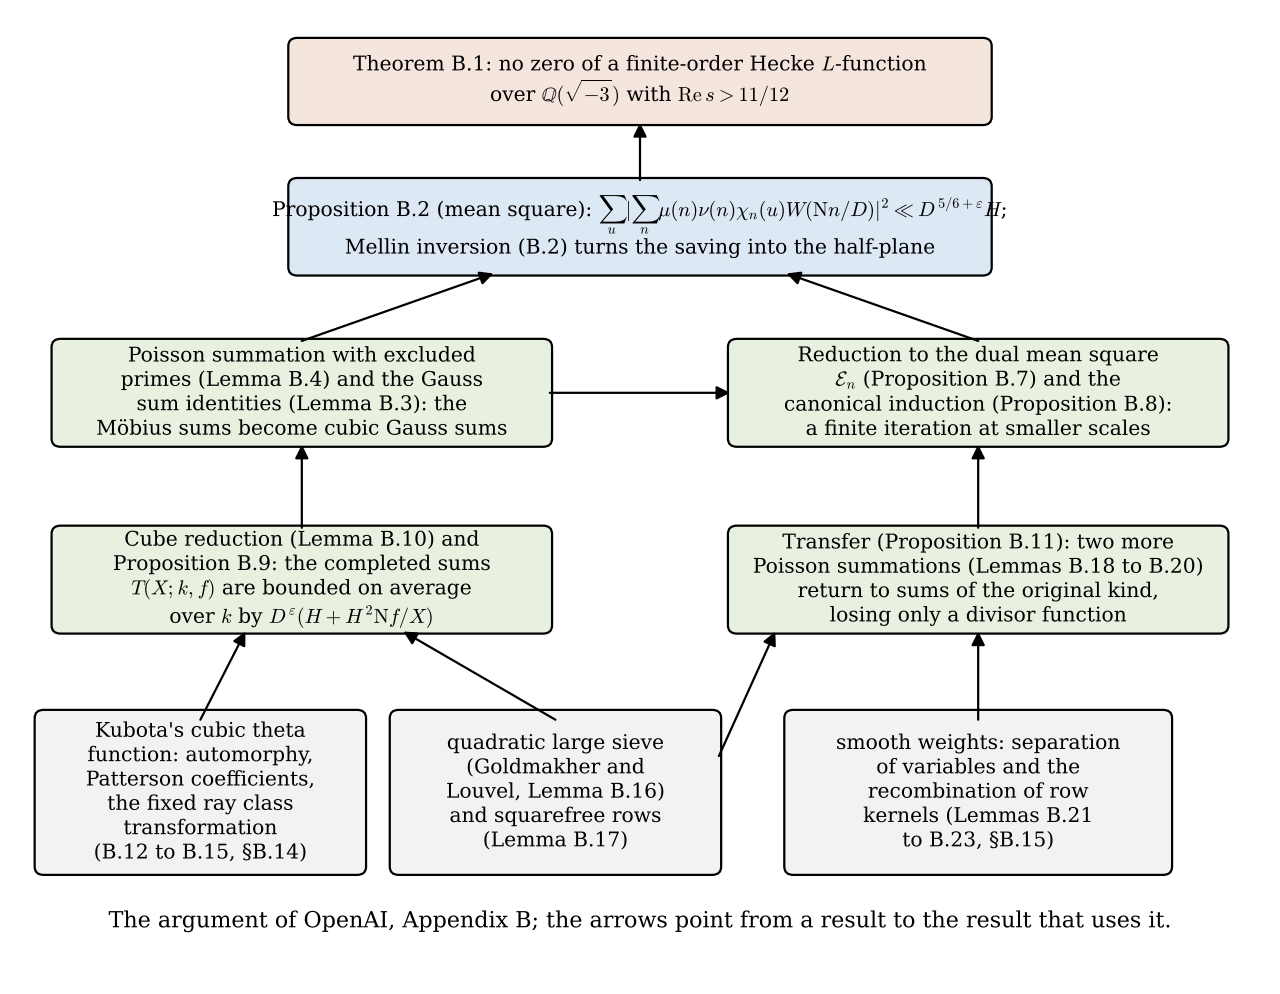
\includegraphics[width=0.9\textwidth]{figures/fig_halfplane.png}
\caption{The structure of the proof of Theorem~\ref{thm:b:main}. The half-plane follows from the mean-square estimate of Proposition~\ref{prop:b:ms}, which is proved by Poisson summation, the canonical induction of Proposition~\ref{prop:b:canonical} and the transfer of Proposition~\ref{prop:b:transfer}; the cubic theta function and the quadratic large sieve enter through Proposition~\ref{prop:b:R}.}
\label{fig:halfplane}
\end{figure}

\subsection{Notation}\label{ssec:b:notation}

Write $\OO=\OO_K=\Z[\omega]$ with $\omega=e^{2\pi i/3}$, and $\NK(a)=a\bar a=|a|^2$ for $a\in K$, $\NK(\mathfrak a)=\#(\OO/\mathfrak a)$ for a nonzero ideal. The ring $\OO$ is Euclidean, so every ideal is principal. An element is \emph{primary} if it is congruent to $1$ modulo $3$; since the six units represent the six invertible classes modulo $3$, an ideal prime to $3$ has a unique primary generator, and we write $\mu(n)$, $\nu(n)$ and so on for the values at the ideal $(n)$. Put $\lambda=1+2\omega$, so that $(\lambda)$ is the prime above $3$ and $\lambda^2$ is a unit times $3$. For a primary prime $p\nmid6$ and $p\nmid u$, $(u/p)_6$ is the sixth root of unity congruent to $u^{(\NK p-1)/6}$ modulo $p$, and $(u/p)_6=0$ for $p\mid u$; this is extended multiplicatively in the denominator to
\[
  \chi_n(u)=\Bigl(\frac un\Bigr)_6\qquad(n\text{ primary},\ (n,6)=1),
\]
with $\chi_1\equiv1$, including at $u=0$. The quadratic and cubic symbols are $\chi_n^3$ and $\chi_n^2$.\footnote{For $j$ an integer, $\chi_p^j$ means the $j$th power on $(\OO/(p))^\times$ extended by zero on the multiples of $p$; in particular $\chi_p^0(x)=\ind_{p\nmid x}$, which is not the constant $1$. This convention matters in the theta transformation of Section~\ref{ssec:b:fixedray}.} Define the additive character
\[
  e(z)=\exp\bigl(4\pi i\operatorname{Im}z/\sqrt3\bigr)\qquad(z\in\C),
\]
which is trivial on $\OO$ and, for primary squarefree $n$ prime to $6$ and an integer $j$, the normalised Gauss sums
\begin{equation}\label{eq:b:gauss}
  \gamma_j(n)=\frac1{\sqrt{\NK n}}\sum_{x\bmod n}\chi_n(x)^je(x/n),\qquad
  \alpha(n)=\frac n{|n|}.
\end{equation}
For $j=-1$ the character is $\bar\chi_n$. We use $\ind_{\mathcal C}$ for the indicator of a condition, $v_p$ for the exponent of a prime, $\tau_{\rm div}(b)$ for the number of ideal divisors of $(b)$, and $\rad\mathfrak r$ for the product of the distinct prime divisors of $\mathfrak r$.

The notation $f\ll g$ means $|f|\le Cg$ with an absolute constant unless subscripts list the parameters the constant may depend on; $f\asymp g$ means $f\ll g\ll f$. A dyadic range is $R\le\NK a<2R$. Throughout, $D\ge2$ is the norm scale of the original M\"obius sum and all other scales are bounded by fixed powers of $D$; we write
\[
  A\precbd B\quad\text{if}\quad A\ll_\varepsilon D^\varepsilon B\ \text{for every }\varepsilon>0,
\]
uniformly in the varying parameters, the constant depending also on the fixed data of each statement. For a compact interval $I\subset(0,\infty)$ and a smooth $W$ supported in $I$, $\|W\|_{C^J(I)}=\max_{j\le J}\sup_I|W^{(j)}|$; for functions of several variables all partial derivatives of total order at most $J$ are taken. A star on a sum restricts the index to squarefree primary elements, prime to the finite set $S$ of primes fixed in the next section.

Finally, the \emph{ray class group} modulo an ideal $\mathfrak m$ is the group of fractional ideals prime to $\mathfrak m$ modulo the principal ideals with a generator congruent to $1$ modulo $\mathfrak m$; a ray class character is a character of this finite group, and the ray class of an element prime to $\mathfrak m$ is the class of the ideal it generates.

\subsection{From the mean-square estimate to the zero-free half-plane}\label{ssec:b:reduction}

Fix a finite-order Hecke character $\nu$ of $K$, extended by zero to the ideals not prime to its conductor, and a finite set $S$ of prime ideals containing the primes above $2$ and $3$ and the primes dividing the conductor of $\nu$. Write $(a,S)=1$ if no prime of $S$ divides $a$. For $W\in C_c^\infty((0,\infty);\C)$ and $u\in\OO$ define the family
\begin{equation}\label{eq:b:family}
  A_u(D)=\sum_{(n,S)=1}\mu(n)\nu(n)\chi_n(u)W(\NK n/D),
\end{equation}
where $n$ runs over the ideals prime to $S$, represented by their primary generators. The untwisted sum is $A_1(D)$. The whole appendix is devoted to the following estimate.

\begin{proposition}\label{prop:b:ms}
For every fixed $0<\vartheta\le1/10$ and $\varepsilon>0$ there is an integer $k=k(\vartheta,\varepsilon)\ge1$ such that for every compact interval $I\subset(0,\infty)$, every smooth $W$ supported in $I$ and every $D\ge2$,
\begin{equation}\label{eq:b:ms}
  \sum_{0<\NK u\le D^{1+\vartheta}}|A_u(D)|^2\ll_{\nu,S,I,\vartheta,\varepsilon}\Bigl(\max_{0\le j\le k}\|W^{(j)}\|_\infty\Bigr)^2D^{2+\vartheta+\varepsilon}.
\end{equation}
\end{proposition}

The proposition is proved in Section~\ref{ssec:b:completion}. We first deduce the theorem from it.

\begin{proof}[Proof of Theorem~\ref{thm:b:main} from Proposition~\ref{prop:b:ms}]
Fix $0<\vartheta\le1/10$ and put $H=D^{1+\vartheta}$, $Y=H^{1/6}$. For a prime ideal $\mathfrak p\notin S$ with $Y/2<\NK\mathfrak p\le Y$ let $p$ be its primary generator. Then $\chi_n(p^6)=\ind_{\mathfrak p\nmid n}$, so $A_1(D)$ and $A_{p^6}(D)$ differ only in the terms with $\mathfrak p\mid n$:
\[
  |A_1(D)-A_{p^6}(D)|\le\|W\|_\infty\,\#\{n:(n,S)=1,\ \mathfrak p\mid n,\ \NK n\asymp D\}\ll_WD/Y.
\]
By Landau's prime ideal theorem~\cite{Lan03} there are $J\asymp Y/\log Y$ such primes, and their sixth powers are distinct rows $u$ of norm at most $H$.\footnote{In a mean square we call the variable of the outer sum the \emph{row} and the variable of the inner sum the \emph{column}; in~\eqref{eq:b:ms} these are $u$ and $n$.} Apply~\eqref{eq:b:ms} with the loss $\varepsilon/2$ and use $\log Y\ll_\varepsilon D^{\varepsilon/2}$:
\begin{equation}\label{eq:b:primeextract}
\begin{aligned}
  |A_1(D)|^2&\le\frac2J\sum_{\substack{Y/2<\NK p\le Y\\(p,S)=1}}|A_{p^6}(D)|^2+O_W\Bigl(\frac{D^2}{Y^2}\Bigr)\\
  &\ll_{\nu,S,W,\vartheta,\varepsilon}\frac{D^{2+\vartheta+\varepsilon}}Y+\frac{D^2}{Y^2}
  =D^{11/6+5\vartheta/6+\varepsilon}+D^{5/3-\vartheta/3}.
\end{aligned}
\end{equation}
Hence $A_1(D)\ll D^{11/12+5\vartheta/12+\varepsilon}$. For a requested exponent loss choose $\vartheta$ and then $\varepsilon$ small, and rename the total loss $\varepsilon$:
\begin{equation}\label{eq:b:mobiussaving}
  A_1(D)\ll_{\nu,S,W,\varepsilon}D^{11/12+\varepsilon}.
\end{equation}

Suppose now that $L_K(s,\nu)$ has a zero $\varrho$ with $\Re\varrho>11/12$. Take $0\ne\phi\in C_c^\infty((1,2))$, $\phi\ge0$, and $W(y)=y^{-\varrho}\phi(y)$. With $\widehat W(s)=\int_0^\infty W(y)y^s\dd y/y$ we have $\widehat W(\varrho)=\int\phi(y)\dd y/y>0$. The function
\[
  \mathcal M_W(s)=\int_0^\infty A_1(D)D^{-s}\frac{\dd D}D
\]
is holomorphic for $\Re s>11/12$, because~\eqref{eq:b:mobiussaving} controls the integral at infinity and $A_1(D)$ vanishes for small $D$ by the compact support of $W$. For $\Re s>1$ termwise integration gives
\[
  \mathcal M_W(s)=\widehat W(s)\sum_{(n,S)=1}\frac{\mu(n)\nu(n)}{\NK n^s}=\frac{\widehat W(s)}{L_K^S(s,\nu)},\qquad
  L_K^S(s,\nu)=L_K(s,\nu)\prod_{\mathfrak p\in S}\bigl(1-\nu(\mathfrak p)\NK\mathfrak p^{-s}\bigr).
\]
By Hecke's continuation theorem~\cite{Hec20} and the identity theorem, $L_K^S(s,\nu)\mathcal M_W(s)=\widehat W(s)$ on $\Re s>11/12$. The omitted Euler factors do not vanish there, so at $s=\varrho$ the left side is $0$ and the right side is $\widehat W(\varrho)>0$, a contradiction.

For a Dirichlet character $\chi$, let $\chi_{-3}$ be the nontrivial character modulo $3$. Quadratic base change gives, up to Euler factors without zeros in $\Re s>0$,
\[
  L_K(s,\chi\circ\NK)=L(s,\chi)L(s,\chi\chi_{-3}),
\]
so the Hecke statement excludes zeros of either factor off $s=1$; at $s=1$ a zero of one factor could only cancel a pole of the other when $\chi$ is principal, and then it would be a zero of $L(1,\chi_{-3})$, which is positive by Dirichlet's theorem~\cite[Chapters~4 and~6]{Dav80}.
\end{proof}

\subsection{The arithmetic identities}\label{ssec:b:arithmetic}

Poisson summation in the row variable will produce the Gauss sums~\eqref{eq:b:gauss}, and the identities of this section convert the M\"obius coefficients into the cubic coefficients
\begin{equation}\label{eq:b:axi}
  a_\xi(n)=\overline{\alpha(n)}\gamma_2(n)\xi(n)\qquad(n\ \text{squarefree primary},\ (n,S)=1),
\end{equation}
where $\xi$ is a ray class character of a fixed modulus. That modulus is chosen once and for all: supported on $S$, divisible by the conductor of $\nu$, and large enough that every reciprocity factor below depends only on the ray class; a function on the ray class group is then a finite linear combination of characters $\xi$ by orthogonality, which is how $\nu$ and the factors $G$, $\mathcal R$ below are absorbed into the twist $\xi$.

\begin{lemma}\label{lem:b:arithmetic}
On the fixed ray class group there are a function $G$ with values in the unit circle and a symmetric $\{\pm1\}$-valued bicharacter $\mathcal R$, that is, $\mathcal R(a,b)=\mathcal R(b,a)$ and $\mathcal R$ is multiplicative in each argument, with the following properties. For primary $a,b,n$ prime to $S$ with $(a,b)=1$ and $n$ squarefree,
\begin{align}
  \chi_b(a)&=\mathcal R(a,b)\chi_a(b),& G(ab)&=G(a)G(b)\mathcal R(a,b),\label{eq:b:recip}\\
  \gamma_2(n)^3&=\mu(n)\alpha(n),& \gamma_1(n)\gamma_2(n)&=\mu(n)\alpha(n)G(n),\label{eq:b:gj}\\
  G(n)&=\overline{\chi_n(4)}\gamma_3(n),& \gamma_1(n)\gamma_{-1}(n)&=\chi_n(-1).\label{eq:b:g}
\end{align}
Consequently, for such $n$ and for coprime squarefree $a,b$,
\begin{align}
  \overline{\alpha(n)}\gamma_2(n)\gamma_1(n)&=\mu(n)G(n),\label{eq:b:convert1}\\
  \mu(n)\gamma_{-1}(n)&=\chi_n(-1)G(n)^{-1}\overline{\alpha(n)}\gamma_2(n),\label{eq:b:convert2}\\
  a_\xi(ab)&=a_\xi(a)a_\xi(b)\chi_b(a)^4,\label{eq:b:crta}\\
  \chi_a(-1)\overline{G(a)}G(b)\mathcal R(a,b)&=G(ba^{-1}),\label{eq:b:quotient}
\end{align}
where the identity for $G(ab)$ extends to all classes of the ray class group and the quotient in~\eqref{eq:b:quotient} is taken there.
\end{lemma}

\begin{proof}
\emph{The Gauss--Jacobi relations~\eqref{eq:b:gj}.} Set $G(n)=\overline{\chi_n(4)}\gamma_3(n)$ for squarefree $n$; that it factors through the ray class group is shown below. Fix a primary prime $p\notin S$ and, for characters $A,B$ of $(\OO/(p))^\times$ extended by zero, the Jacobi sum $J(A,B)=\sum_{x\bmod p}A(x)B(1-x)$. The substitution $u=2x-1$ shows that $4x(1-x)=y$ has $1+\chi_p^3(1-y)$ solutions $x$ modulo $p$, so
\[
  \chi_p(4)J(\chi_p,\chi_p)=\sum_x\chi_p\bigl(4x(1-x)\bigr)=\sum_y\chi_p(y)\bigl(1+\chi_p^3(1-y)\bigr)=J(\chi_p,\chi_p^3).
\]
The Gauss--Jacobi identity $\gamma_1\gamma_3/\gamma_4=J(\chi_p,\chi_p^3)/\sqrt{\NK p}$ (see~\cite[(3.18)]{IK04}) and the same identity for $J(\chi_p,\chi_p)$ give
\[
  \frac{\gamma_1(p)\gamma_3(p)}{\gamma_4(p)}=\chi_p(4)\frac{\gamma_1(p)^2}{\gamma_2(p)}.
\]
For $j\not\equiv0\pmod6$ one has $\gamma_j(p)\gamma_{-j}(p)=\chi_p(-1)^j$; with $j=2$ this is $\gamma_2(p)\gamma_4(p)=1$, as $\chi_p^2$ is cubic. Cancelling $\gamma_1(p)$ and rearranging,
\[
  \gamma_1(p)\gamma_2(p)=\overline{\chi_p(4)}\gamma_3(p)\gamma_2(p)^3.
\]
It remains to evaluate $\gamma_2(p)^3=\gamma_2(p)^2/\gamma_4(p)=J(\chi_p^2,\chi_p^2)/\sqrt{\NK p}$. Put $q=\NK p$. The Jacobi sum lies in $\OO$ and has norm $q$. Reducing modulo $p$ and expanding the binomial,
\[
  J(\chi_p^2,\chi_p^2)\equiv\sum_x x^{\frac{q-1}3}(1-x)^{\frac{q-1}3}=\sum_{\ell=0}^{(q-1)/3}(-1)^\ell\binom{(q-1)/3}\ell\sum_xx^{\frac{q-1}3+\ell}\equiv0\pmod p,
\]
since each exponent $(q-1)/3+\ell$ lies strictly between $0$ and $q-1$. So $J(\chi_p^2,\chi_p^2)$ is a unit times $p$. Write $\chi_p^2(x(1-x))=\omega^{j_x}$ for $x\ne0,1$; the product of all $x(1-x)$ is $1$, so $\sum j_x\equiv0\pmod3$, and since $(\omega-1)^2$ generates $(3)$,
\[
  J(\chi_p^2,\chi_p^2)=\sum_{x\ne0,1}\omega^{j_x}\equiv(q-2)+(\omega-1)\sum_{x\ne0,1}j_x\equiv-1\pmod3.
\]
With $p\equiv1\pmod3$ this fixes the unit: $J(\chi_p^2,\chi_p^2)=-p$, so $\gamma_2(p)^3=-\alpha(p)$. The Chinese remainder theorem extends both prime identities to squarefree $n$, one sign $-1$ for each prime factor giving $\mu(n)$.\footnote{The Chinese remainder theorem gives $\gamma_j(ab)=\gamma_j(a)\gamma_j(b)\chi_a(b)^j\chi_b(a)^j$ for coprime $a,b$; for $j=2$ cubic reciprocity makes the two symbols equal, and for the products of two sums with $j+j'\equiv0$ the symbols cancel.}

\emph{The identity~\eqref{eq:b:crta}.} For coprime squarefree primary $a,b$ prime to $S$, $\gamma_2(ab)=\gamma_2(a)\gamma_2(b)\chi_a(b)^2\chi_b(a)^2$, and cubic reciprocity gives $\chi_a(b)^2=\chi_b(a)^2$; multiplying by $\overline{\alpha(ab)}\xi(ab)$ gives~\eqref{eq:b:crta}.

\emph{Reciprocity~\eqref{eq:b:recip} and the first identity of~\eqref{eq:b:g}.} For $c\in\OO$ prime to $2$ we show
\begin{equation}\label{eq:b:quadgauss}
  \Gamma_{\rm quad}(c):=|c|^{-1}\sum_{x\bmod c}e(x^2/c)=\frac12\sum_{y\bmod2\OO}e(-cy^2/4).
\end{equation}
Apply Poisson summation over $z\in\OO$ to $e(z^2/c)e^{-\pi\eta|z|^2}$, $\eta>0$. The Fourier transform of this product is
\[
  \frac{|c|}{2\sqrt{r_\eta}}e^{-\pi\eta\NK(c)|y|^2/(4r_\eta)}e\bigl(-cy^2/(4r_\eta)\bigr),\qquad r_\eta=1+3\NK(c)\eta^2/16.
\]
Divide both sides by the Gaussian mass $\sum_ze^{-\pi\eta|z|^2}\asymp\eta^{-1}$. Replacing $r_\eta$ by $1$ on the Fourier side changes it by $O_c(\eta^2\sum_y|y|^2e^{-C_c\eta|y|^2})=O_c(1)$, which is $O_c(\eta)$ after the division. Group the original sum modulo $c$ and the Fourier sum modulo $2\OO$ and let $\eta\downarrow0$ to get~\eqref{eq:b:quadgauss}. For $c=a+b\omega$ it reads
\[
  \Gamma_{\rm quad}(a+b\omega)=\tfrac12\bigl(1+i^{-b}+i^a+i^{b-a}\bigr),
\]
so $\Gamma_{\rm quad}(c)$ depends only on $c$ modulo $4\OO$ and is invariant under multiplication by squares of $(\OO/4\OO)^\times$; on the four square classes $1,-1,\lambda,-\lambda$ it takes the values $1,1,i,-i$. Hence
\[
  \begin{gathered}
  \mathcal R(c_1,c_2):=\frac{\Gamma_{\rm quad}(c_1c_2)}{\Gamma_{\rm quad}(c_1)\Gamma_{\rm quad}(c_2)},\\
  \mathcal R\bigl((-1)^e\lambda^f,(-1)^g\lambda^h\bigr)=(-1)^{eh+fg+fh}\quad(e,f,g,h\in\{0,1\}),
  \end{gathered}
\]
is a symmetric bicharacter on these classes. For a prime $p$ every $y$ has $1+\chi_p^3(y)$ square roots, so grouping by $y=x^2$ and using $\sum_ye(y/p)=0$ gives $\Gamma_{\rm quad}(p)=\gamma_3(p)$, and the Chinese remainder theorem extends this to squarefree $n$. With cubic reciprocity this identifies $\mathcal R$ with the quotient $\chi_b(a)/\chi_a(b)$ for coprime primary $a,b$. Since $\chi_c(4)=(-2/c)_3=(c/(-2))_3$ is a character modulo $2$, the function $G(c)=\overline{\chi_c(4)}\Gamma_{\rm quad}(c)$ factors through the fixed ray class group and satisfies~\eqref{eq:b:recip}, with $\mathcal R(c,c)=\chi_c(-1)$.

\emph{The quotient~\eqref{eq:b:quotient}.} In the ray class group the multiplicativity of $G$ gives $G(a^{-1})=\chi_a(-1)\overline{G(a)}$, and then $G(ba^{-1})=G(b)G(a^{-1})\mathcal R(b,a^{-1})=\chi_a(-1)\overline{G(a)}G(b)\mathcal R(a,b)$ by the symmetry and multiplicativity of $\mathcal R$.

\emph{The conversions.} The second identity of~\eqref{eq:b:g} is the inverse-character Gauss identity. Multiplying the second identity of~\eqref{eq:b:gj} by $\overline{\alpha(n)}$ gives~\eqref{eq:b:convert1}, and combining it with $\gamma_1\gamma_{-1}=\chi_n(-1)$ gives~\eqref{eq:b:convert2}.
\end{proof}

Under Poisson summation, \eqref{eq:b:convert2} converts the M\"obius coefficients into $a_\xi(n)$, up to fixed ray class factors, and \eqref{eq:b:convert1} converts them back.

\subsection{Poisson summation with excluded primes}\label{ssec:b:poisson}

The row sums to which Poisson summation is applied carry a coprimality condition, and we record the formula with that condition included, so that its effect on the frequencies and on the normalisation is visible. In quotients and Gauss sums every ideal is represented by a fixed generator, primary when the ideal is prime to $3$.

\begin{lemma}\label{lem:b:poisson}
Let $\mathcal H>0$, let $\mathfrak r$ be a nonzero ideal, let $\Phi(\NK k/\mathcal H)$ be a smooth radial Schwartz weight on $\OO$, and let $\chi$ be a primitive character of $(\OO/\mathfrak m)^\times$, viewed as a function on $\OO$ by reduction modulo $\mathfrak m$ and extension by zero. Write $\gamma(\chi)=\NK\mathfrak m^{-1/2}\sum_{x\bmod\mathfrak m}\chi(x)e(x/\mathfrak m)$ for its normalised Gauss sum. Then
\begin{equation}\label{eq:b:poisson}
  \sum_{k\in\OO}\chi(k)\ind_{(k,\mathfrak r)=1}\Phi(\NK k/\mathcal H)
  =\frac{\mathcal H\gamma(\chi)}{\sqrt{\NK\mathfrak m}}\sum_{d\mid\rad\mathfrak r}\frac{\mu(d)\chi(d)}{\NK d}\sum_{h\in\OO}\overline{\chi(h)}\,\widehat\Phi\Bigl(\frac{\mathcal H\NK h}{\NK d\,\NK\mathfrak m}\Bigr),
\end{equation}
where $\widehat\Phi(|w|^2)=\frac2{\sqrt3}\int_\C\Phi(|z|^2)e(-zw)\dd x\dd y$, the measure giving $\OO$ covolume one. If $\chi$ is nonprincipal then $\overline{\chi(0)}=0$ and the zero frequency contributes nothing; for the principal primitive character ($\mathfrak m=1$) the zero frequency contributes $\mathcal H\widehat\Phi(0)\prod_{\mathfrak p\mid\mathfrak r}(1-\NK\mathfrak p^{-1})$.
\end{lemma}

\begin{proof}
Inclusion--exclusion and $k=d\ell$ give
\[
  \sum_k\chi(k)\ind_{(k,\mathfrak r)=1}\Phi(\NK k/\mathcal H)=\sum_{d\mid\rad\mathfrak r}\mu(d)\chi(d)\sum_\ell\chi(\ell)\Phi\Bigl(\frac{\NK\ell}{\mathcal H/\NK d}\Bigr).
\]
Apply Poisson summation on the lattice $\OO$ in $\ell$, on the residue classes modulo $\mathfrak m$, at the scale $\mathcal H/\NK d$~\cite[Theorem~4.5]{IK04}; the finite Fourier transform of a primitive character is $\sqrt{\NK\mathfrak m}\,\gamma(\chi)\overline{\chi(h)}$ for every $h$~\cite[(3.12)]{IK04}, which gives~\eqref{eq:b:poisson}. The statements about the zero frequency follow by summing $\mu(d)/\NK d$ over $d\mid\rad\mathfrak r$.
\end{proof}

\subsection{The dual mean square}\label{ssec:b:dual}

\begin{definition}\label{def:b:energy}
Let $\mathcal H,X,F>0$ be the norm scales of the row $k\in\OO$, the column $n$ and an auxiliary index $f$. For a ray class character $\xi$ and a smooth compactly supported $W$ on $(0,\infty)$ the \emph{dual mean square} is
\begin{equation}\label{eq:b:energy}
  \En(\mathcal H,X,F;\xi,W)=\frac1{XF}\sfstar_{\substack{F\le\NK f<2F\\(f,S)=1}}\ \sum_{0<\NK k\le\mathcal H}\Bigl|\sfstar_{(n,S)=1}a_\xi(n)\chi_n(k)\chi_n(f)^4W(\NK n/X)\Bigr|^2.
\end{equation}
\end{definition}

The twist $\chi_n(f)^4$ will arise from the common factors of two columns; note that $\chi_n(f)^4$ enforces $(n,f)=1$ since $\chi_n(f)=0$ otherwise. Write $\En_{\mathfrak r}$ for the same expression with the further restriction $(n,\mathfrak r)=1$ on the column. The restriction is removed at the cost of a divisor factor, without changing the row range or the product $XF$.

\begin{lemma}\label{lem:b:remove}
Let $r_0$ be the product of the primes dividing $\mathfrak r$ outside $S$. For $\mathcal H,X>0$, $F\ge1$ and smooth compactly supported $W$,
\begin{equation}\label{eq:b:remove}
  \En_{\mathfrak r}(\mathcal H,X,F;\xi,W)\le\tau_{\rm div}(r_0)\sum_{d\mid r_0}\En\Bigl(\mathcal H,\frac X{\NK d},F\NK d;\xi,W\Bigr).
\end{equation}
\end{lemma}

\begin{proof}
Let $C_{\mathfrak r}(X;k,f)$ be the inner column sum of $\En_{\mathfrak r}$. Inclusion--exclusion over $d\mid r_0$, the substitution $n=dm$ and~\eqref{eq:b:crta} give
\[
\begin{aligned}
  C_{\mathfrak r}(X;k,f)&=\sum_{d\mid r_0}\mu(d)\sfstar_{\substack{(n,S)=1\\d\mid n}}a_\xi(n)\chi_n(k)\chi_n(f)^4W(\NK n/X)\\
  &=\sum_{\substack{d\mid r_0\\(d,f)=1}}\mu(d)a_\xi(d)\chi_d(k)\chi_d(f)^4\,C_1(X/\NK d;k,df),
\end{aligned}
\]
because $\chi_m(d)^4$ enforces $(m,d)=1$ and combines with $\chi_m(f)^4$ into $\chi_m(df)^4$, while the terms with $(d,f)\ne1$ vanish. Each coefficient in front of $C_1$ has modulus at most one. Cauchy--Schwarz in $d$ gives the factor $\tau_{\rm div}(r_0)$, and enlarging the injective image $f\mapsto df$ to the whole squarefree range $F\NK d\le\NK(df)<2F\NK d$ gives the terms on the right of~\eqref{eq:b:remove}; the normalisation is unchanged since $(X/\NK d)(F\NK d)=XF$.
\end{proof}

\subsection{Reduction to the dual mean square}\label{ssec:b:poissonreduction}

\begin{proposition}\label{prop:b:poissonreduction}
Fix $0<\vartheta\le1/10$ and put $H=D^{1+\vartheta}$. For each fixed $C\ge1$ and all real $B,F\ge1$ consider the ranges
\begin{equation}\label{eq:b:initialscales}
  X=\frac D{BF},\qquad0<\mathcal H\le\frac{CD^2}{HB^2},\qquad XF=\frac DB.
\end{equation}
Suppose that for every $\varepsilon>0$ there is an integer $J=J(\vartheta,\varepsilon)\ge1$ such that, for every compact interval $I\subset(0,\infty)$ and every smooth $W$ supported in $I$,
\begin{equation}\label{eq:b:auxtarget}
  \En(\mathcal H,X,F;\xi,W)\ll_{\nu,S,I,C,\vartheta,\varepsilon}\|W\|_{C^J(I)}^2D^\varepsilon XF.
\end{equation}
Then Proposition~\ref{prop:b:ms} holds.
\end{proposition}

\begin{proof}
Write $I=[a_0,b_0]$ and $N=\NK$. Choose a nonnegative radial Schwartz weight $\Phi$ with $\Phi\ge1$ on $[0,1]$ and $\operatorname{supp}\widehat\Phi\subset[0,C_\Phi]$ for a fixed $C_\Phi>0$.\footnote{Such a weight is the square of a real radial Schwartz function with compactly supported Fourier transform, rescaled; its Fourier transform is then a convolution of compactly supported functions and is itself compactly supported.} It suffices to prove $\mathcal M_D\ll\|W\|^2_{C^{J'}(I)}HD^\varepsilon$ for some $J'=J'(\vartheta,\varepsilon)$, where
\begin{equation}\label{eq:b:expandedms}
  \mathcal M_D=\frac1D\sum_{u\in\OO}\Phi(N(u)/H)\Bigl|\sum_{(n,S)=1}\mu(n)\nu(n)\chi_n(u)W(N(n)/D)\Bigr|^2,
\end{equation}
since the left side of~\eqref{eq:b:ms} is at most $D\mathcal M_D$.

\emph{Expanding the square.} Conjugate the inner sum, expand, and put $g=(n_1,n_2)$, $n_j=gz_j$; the squarefree indices satisfy $(z_1,z_2)=(z_1z_2,g)=1$ and $\overline{\chi_{n_1}(u)}\chi_{n_2}(u)=\ind_{(u,g)=1}\overline{\chi_{z_1}(u)}\chi_{z_2}(u)$. The character $\chi=\overline{\chi_{z_1}}\chi_{z_2}$ is primitive modulo $z_1z_2$, so Lemma~\ref{lem:b:poisson} with the exclusion $g$ gives
\begin{equation}\label{eq:b:initialrows}
  \sum_u\Phi(N(u)/H)\ind_{(u,g)=1}\chi(u)=\sum_{e\mid g}\frac{H\mu(e)\chi(e)\gamma(\chi)}{N(e)\sqrt{N(z_1)N(z_2)}}\sum_h\overline{\chi(h)}\,\widehat\Phi\Bigl(\frac{HN(h)}{N(e)N(z_1)N(z_2)}\Bigr).
\end{equation}
The zero frequency occurs only for $z_1=z_2=1$ and contributes
\[
  Z=\frac HD\widehat\Phi(0)\sfstar_{(g,S)=1}|W(N(g)/D)|^2\prod_{p\mid g}\Bigl(1-\frac1{N(p)}\Bigr)\ll_{\Phi,I}H\|W\|_\infty^2.
\]
All $h\ne0$ are retained, including those with $z_1=z_2=1$.

\emph{Converting the coefficients.} Expand the fixed ray class function $\overline{\nu(t)}G(t^{-1})=\sum_\xi c_\xi\xi(t)$. The Chinese remainder theorem and~\eqref{eq:b:convert2}, \eqref{eq:b:quotient} give\footnote{By the Chinese remainder theorem the Gauss sum factors as $\gamma(\overline{\chi_{z_1}}\chi_{z_2})=\gamma_{-1}(z_1)\gamma_1(z_2)\overline{\chi_{z_1}(z_2)}\chi_{z_2}(z_1)$. Convert $\mu(z_1)\gamma_{-1}(z_1)$ by~\eqref{eq:b:convert2} and $\mu(z_2)\gamma_1(z_2)$ by~\eqref{eq:b:convert1}. The ray class factors then collect, by~\eqref{eq:b:quotient} with $t=z_1z_2^{-1}$, into $\chi_{z_1}(-1)G(z_1)^{-1}G(z_2)\mathcal R(z_1,z_2)\overline{\nu(z_1)}\nu(z_2)$, which equals $\overline{\nu(t)}G(t^{-1})$.}
\begin{equation}\label{eq:b:pairedgauss}
  \mu(z_1)\mu(z_2)\overline{\nu(z_1)}\nu(z_2)\gamma(\overline{\chi_{z_1}}\chi_{z_2})=\sum_\xi c_\xi a_\xi(z_1)\overline{a_\xi(z_2)}.
\end{equation}
Put $W_0(x)=x^{-1/2}\overline{W(x)}$. Substituting~\eqref{eq:b:pairedgauss} into~\eqref{eq:b:initialrows}, with the factor $1/D$ of~\eqref{eq:b:expandedms},
\[
  \mathcal M_D-Z=\sum_\xi c_\xi\mathcal S_\xi,\qquad|\mathcal M_D-Z|\ll\max_\xi|\mathcal S_\xi|,
\]
the sum over $\xi$ being finite and fixed. Fix $\xi$. Using $\overline{\chi_z(e)}=\chi_z(e^5)$,
\[
\begin{aligned}
  \mathcal S_\xi=\frac H{D^2}\sfstar_g\sum_{e\mid g}\frac{\mu(e)N(g)}{N(e)}\sum_{h\ne0}\sfstar_{\substack{z_1,z_2\\(z_1,z_2)=1\\(z_1z_2,g)=1}}&a_\xi(z_1)\overline{a_\xi(z_2)}\chi_{z_1}(he^5)\overline{\chi_{z_2}(he^5)}\\
  &\times W_0\Bigl(\frac{N(gz_1)}D\Bigr)\overline{W_0\Bigl(\frac{N(gz_2)}D\Bigr)}\widehat\Phi\Bigl(\frac{HN(h)}{N(e)N(z_1)N(z_2)}\Bigr),
\end{aligned}
\]
where starred variables are squarefree, primary and prime to $S$, and $h,k$ range over nonzero elements of $\OO$. We must show $|\mathcal S_\xi|\ll\|W\|^2_{C^{J'}(I)}HD^\varepsilon$.

\emph{Removing the coprimality of the columns.} Insert $\ind_{(z_1,z_2)=1}=\sum_{v\mid z_1,v\mid z_2}\mu(v)$ and put $z_j=vm_j$. By~\eqref{eq:b:crta} the common factor satisfies $a_\xi(vm)=a_\xi(v)a_\xi(m)\chi_m(v)^4$ and $|a_\xi(v)\chi_v(he^5)|^2=\ind_{(v,h)=1}$, with $(v,e)=1$. Thus
\begin{multline*}
  \mathcal S_\xi=\frac H{D^2}\sfstar_{\substack{g,v\\(g,v)=1}}\sum_{e\mid g}\frac{\mu(e)\mu(v)N(g)}{N(e)}\sum_{\substack{h\ne0\\(h,v)=1}}\sfstar_{\substack{m_1,m_2\\(m_1m_2,gv)=1}}a_\xi(m_1)\overline{a_\xi(m_2)}\\
  \times\chi_{m_1}(he^5v^4)\overline{\chi_{m_2}(he^5v^4)}\,W_0\Bigl(\frac{N(gvm_1)}D\Bigr)\overline{W_0\Bigl(\frac{N(gvm_2)}D\Bigr)}\widehat\Phi\Bigl(\frac{HN(h)}{N(e)N(v)^2N(m_1)N(m_2)}\Bigr),
\end{multline*}
with no restriction $(m_1,m_2)=1$ left. Make the bijective change of variables
\[
  b=g/e,\quad f=ev,\quad k=eh;\qquad e=(f,k),\quad v=f/e,\quad g=be,\quad h=k/e.
\]
Then $b,f$ are coprime and squarefree, $k\ne0$ is arbitrary, $gv=bf$, $he^5v^4=kf^4$, $\mu(e)\mu(v)=\mu(f)$ and $N(g)/N(e)=N(b)$, so
\begin{multline}\label{eq:b:columnoutput}
  \mathcal S_\xi=\frac H{D^2}\sfstar_{\substack{b,f\\(b,f)=1}}\mu(f)N(b)\sum_{k\ne0}\sfstar_{\substack{m_1,m_2\\(m_1m_2,b)=1}}a_\xi(m_1)\overline{a_\xi(m_2)}\chi_{m_1}(kf^4)\overline{\chi_{m_2}(kf^4)}\\
  \times W_0\Bigl(\frac{N(bfm_1)}D\Bigr)\overline{W_0\Bigl(\frac{N(bfm_2)}D\Bigr)}\widehat\Phi\Bigl(\frac{HN(k)}{N(f)^2N(m_1)N(m_2)}\Bigr).
\end{multline}
The characters enforce $(m_j,f)=1$, so only the exclusion $(m_j,b)=1$ is displayed. The supports give $N(b)N(f)\le b_0D$ and $0<N(k)\le C_\Phi b_0^2D^2/(HN(b)^2)$.

\emph{Dyadic ranges and the smooth weights.} Partition $B\le N(b)<2B$ and $F\le N(f)<2F$ dyadically, write $\mathcal S_{\xi;B,F}$ for the corresponding part of~\eqref{eq:b:columnoutput}, and put
\[
  X=\frac D{BF},\qquad\mathcal H=\frac{C_{I,\Phi}D^2}{HB^2},\qquad C_{I,\Phi}=\max(2,C_\Phi b_0^2),
\]
which satisfy~\eqref{eq:b:initialscales}. In the variables $x_j=N(m_j)/X$ the coupled weight is
\[
  \begin{gathered}
  \mathcal K_{b,f,k}(x_1,x_2)=W_0(rx_1)\overline{W_0(rx_2)}\,\widehat\Phi\Bigl(\frac a{x_1x_2}\Bigr),\\
  r=\frac{N(b)N(f)}{BF}\in[1,4),\qquad a=\frac{HN(k)}{N(f)^2X^2}\le C_{I,\Phi},
  \end{gathered}
\]
and for every integer $q\ge0$ these kernels satisfy $\sup_{b,f,k}\|\mathcal K_{b,f,k}\|_{C^q([a_0/4,b_0]^2)}\ll_{I,\Phi,q}\|W\|^2_{C^q(I)}$. For $U\in C_c^\infty(I_*)$, $I_*=[a_0/8,2b_0]$, put
\[
  S_U(b,f,k)=\sfstar_{\substack{(n,S)=1\\(n,b)=1}}a_\xi(n)\chi_n(k)\chi_n(f)^4U(N(n)/X).
\]
The shifts $(X,F)\mapsto(X/N(d),FN(d))$ preserve~\eqref{eq:b:initialscales}, so Lemma~\ref{lem:b:remove} and the hypothesis~\eqref{eq:b:auxtarget} with $J=J(\vartheta,\varepsilon/4)$ give
\[
\begin{aligned}
  \sum_{f,k}|S_U(b,f,k)|^2&=XF\,\En_{(b)}(\mathcal H,X,F;\xi,U)\\
  &\le XF\tau_{\rm div}(b)\sum_{d\mid b}\En(\mathcal H,X/N(d),FN(d);\xi,U)\ll D^{\varepsilon/2}(XF)^2\|U\|^2_{C^J(I_*)},
\end{aligned}
\]
the divisor factor being absorbed in $D^{\varepsilon/4}$ since $N(b)\ll_ID$. Now Lemma~\ref{lem:b:smoothms} below turns a mean-square bound for every common test function $U$ into a bound for the quadratic form with the row-dependent kernel $\mathcal K_{b,f,k}$, at the cost of the $C^{2J+4}$ norm of the kernel. Apply it for each fixed $b$ with row index $(f,k)$, coefficient $\mu(f)\ind_{(f,b)=1}$ and kernel $\mathcal K_{b,f,k}$; the larger row range $0<N(k)\le\mathcal H$ only adds rows whose kernel vanishes. With $q=2J+4$,
\begin{multline}\label{eq:b:weighted}
  |\mathcal S_{\xi;B,F}|\ll D^{\varepsilon/2}\|W\|^2_{C^q(I)}\sfstar_{B\le N(b)<2B}\frac{HN(b)}{D^2}(XF)^2\\
  \ll D^{\varepsilon/2}\|W\|^2_{C^q(I)}\frac{HB^2(XF)^2}{D^2}=D^{\varepsilon/2}\|W\|^2_{C^q(I)}H,
\end{multline}
since $XF=D/B$ and there are $O(B)$ ideals $b$ in the range. Summing the $O((\log D)^2)$ nonempty dyadic ranges bounds $\mathcal S_\xi$, summing over the finite set of $\xi$ and adding $Z$ bounds $\mathcal M_D$, and multiplying by $D$ gives~\eqref{eq:b:ms}; the derivative order depends only on $\vartheta$ and $\varepsilon$.
\end{proof}

\subsection{The completed sums and the two inputs}\label{ssec:b:inputs}

Put $\Sigma=XF$. The dual mean square is bounded by the following proposition, whose proof occupies Sections~\ref{ssec:b:inputs} to~\ref{ssec:b:transferproof}.

\begin{proposition}\label{prop:b:canonical}
Fix $\kappa>0$ and $C_0\ge1$, and suppose that
\begin{equation}\label{eq:b:positivegap}
  \mathcal H,X,F\ge1,\qquad\Sigma=XF\le D^{C_0},\qquad\mathcal H\le\Sigma D^{-\kappa}.
\end{equation}
For every $\varepsilon>0$ there is an integer $J=J(\kappa,C_0,\varepsilon)\ge1$ such that
\begin{equation}\label{eq:b:canonical}
  \En(\mathcal H,X,F;\xi,W)\ll_{I,\nu,S,\kappa,C_0,\varepsilon}\|W\|^2_{C^J(I)}D^\varepsilon\Sigma
\end{equation}
for every compact interval $I\subset(0,\infty)$ and every smooth $W$ supported in $I$.
\end{proposition}

\emph{The completed sums.} Let $\Psi$ be a completely multiplicative function on the ideals prime to $3$, vanishing on the ideals divisible by a prime of $S$, and write $\Psi(n)=\Psi((n))$ for primary $n$. Define
\begin{equation}\label{eq:b:T}
  T(X;\Psi)=\sfstar_{(n,S)=1}\ \sum_{\substack{b\equiv1\ (3)\\(b,S)=1}}\frac{\overline{\alpha(n)}\gamma_2(n)\Psi(n)\,\overline{\alpha(b)}^{\,3}\Psi(b)^3}{\sqrt{\NK n}\,\NK b}\,V_*\bigl(\NK n\,\NK b^3/X\bigr),\qquad V_*(y)=\sqrt y\,W(y),
\end{equation}
where $n$ is squarefree and $b$ is any primary element prime to $S$. The index $b$ supplies the cubes that occur in the Fourier expansion of the cubic theta function, and the $b=1$ part is $X^{-1/2}\sfstar_n\overline{\alpha(n)}\gamma_2(n)\Psi(n)W(\NK n/X)$. For a ray class character $\xi$, a nonzero row $k\in\OO$ and a squarefree primary $f$ prime to $S$ put
\begin{equation}\label{eq:b:completedtwist}
  \Psi_k(n)=\xi(n)\chi_n(k)\chi_n(f)^4\ \text{ for }(n,S)=1,\quad\Psi_k(n)=0\ \text{ otherwise},\quad T(X;k,f)=T(X;\Psi_k),
\end{equation}
so that the $b=1$ part of $T(X;k,f)$ is $X^{-1/2}$ times the column sum of~\eqref{eq:b:energy}.

\emph{The completed mean-square estimate.} The theta transformation turns the sextic twists of $\Psi_k$ into quadratic characters, and the quadratic large sieve then gives the following estimate, proved in Section~\ref{ssec:b:squarefreerows}.

\begin{proposition}\label{prop:b:R}
Fix $\varepsilon>0$, $C_0\ge1$ and a character $\xi$ of the fixed ray class group. There is $J=J(\varepsilon,C_0)\ge1$ such that
\begin{equation}\label{eq:b:R}
  \sum_{0<\NK k\ll\mathcal H}|T(X;k,f)|^2\ll_{I,\xi,S,\varepsilon,C_0}D^\varepsilon\|W\|^2_{C^J(I)}\Bigl(\mathcal H+\frac{\mathcal H^2\NK f}X\Bigr)
\end{equation}
whenever $1\le\mathcal H,X,\NK f\le D^{C_0}$, for $f$ squarefree primary with $(f,S)=1$, $W$ smooth and supported in a compact $I\subset(0,\infty)$, and $T$ as in~\eqref{eq:b:completedtwist}.
\end{proposition}

\emph{Cube inversion.} Set
\begin{equation}\label{eq:b:cubecutoff}
  H_c^3=\min\Bigl(X,\frac{X^2}{\mathcal H^2}\Bigr),\qquad L_b=\frac X{\NK b^3}.
\end{equation}

\begin{lemma}\label{lem:b:cubereduction}
Fix $C_0\ge1$ and $\varepsilon>0$, and suppose $1\le\mathcal H,X,F\le D^{C_0}$ and $\mathcal H\le\Sigma=XF$. There is an integer $J=J(\varepsilon,C_0)\ge1$ such that
\begin{equation}\label{eq:b:cubereduction}
  \En(\mathcal H,X,F;\xi,W)\ll_{I,\nu,S,C_0,\varepsilon}D^\varepsilon\Bigl(\Sigma\|W\|^2_{C^J(I)}+\sup_{\substack{b\equiv1\ (3),\ (b,S)=1\\\NK b>H_c,\ L_b>1}}\En(\mathcal H,L_b,F;\xi,W)\Bigr)
\end{equation}
for every compact $I\subset(0,\infty)$ and $W\in C_c^\infty(I)$. An empty supremum is zero, and it is empty when $\mathcal H^2\le X$.
\end{lemma}

\begin{proof}
Write $N=\NK$ and $I=[u,v]$. Complete multiplicativity, including at the zeros of $\Psi_k$, gives the M\"obius inversion
\begin{equation}\label{eq:b:cubeinverse}
  X^{-1/2}\sfstar_{(n,S)=1}a_\xi(n)\chi_n(k)\chi_n(f)^4W(N(n)/X)=\sum_{(h,S)=1}\frac{\mu(h)\overline{\alpha(h)}^{\,3}\Psi_k(h)^3}{N(h)}\,T\bigl(X/N(h)^3;k,f\bigr):
\end{equation}
after substituting~\eqref{eq:b:T} the coefficient of the total cube index $b$ contains $\sum_{h\mid b}\mu(h)=\ind_{b=1}$.\footnote{The weight $w_k(b)=\overline{\alpha(b)}^3\Psi_k(b)^3$ is completely multiplicative, so $w_k(h)w_k(b/h)=w_k(b)$ even when $h$ and $b/h$ share prime factors, which is what makes the inversion exact; compare~\cite[(1.18)]{IK04} and~\cite[(8.2)]{DR}. One cannot simply discard the terms $b\ne1$ of $T$, because the contributions of different $b$ can cancel.}

Split the right side into $P_{\rm short}(k,f)$, the terms with $N(h)\le H_c$, and $P_{\rm long}(k,f)$, the rest, and let $\En_{\rm short}$, $\En_{\rm long}$ be the corresponding mean squares $F^{-1}\sfstar_f\sum_k|P|^2$. Weighted Cauchy--Schwarz for each $k,f$ and Proposition~\ref{prop:b:R}, with the exponent $\varepsilon/4$ and the range $C_0+1$ (since $N(f)<2D^{C_0}$), give
\begin{equation}\label{eq:b:shortcube}
\begin{aligned}
  \En_{\rm short}&\le\Bigl(\sum_{N(h)\le H_c}\frac1{N(h)}\Bigr)\sum_{N(h)\le H_c}\frac1{N(h)}\,\frac1F\sfstar_{\substack{F\le N(f)<2F\\(f,S)=1}}\sum_{0<N(k)\le\mathcal H}|T(X/N(h)^3;k,f)|^2\\
  &\ll D^{\varepsilon/2}\|W\|^2_{C^J(I)}\Bigl(\mathcal H+\frac{\mathcal H^2FH_c^3}X\Bigr)\ll D^{\varepsilon/2}\Sigma\|W\|^2_{C^J(I)},
\end{aligned}
\end{equation}
where $X/N(h)^3\ge1$, the reciprocal norm sum is a logarithm, and the last step uses $\mathcal H\le\Sigma$ and $H_c^3\le X^2/\mathcal H^2$. If $H_c<1$ the short sum is empty.

In the long part expand $T$ by~\eqref{eq:b:T} with the cube index $c$, put $b=hc$, and note that the pairs giving $b$ are the $(h,b/h)$ with $h\mid b$, $N(h)>H_c$, and that $\Psi_k(b)^3=\xi(b)^3\chi_b(k)^3\ind_{(b,f)=1}$. This gives
\[
  \begin{gathered}
  P_{\rm long}(k,f)=\sum_{\substack{(b,S)=1\\N(b)>H_c}}\frac{\beta_0(b,f)\chi_b(k)^3}{N(b)}\,\frac1{\sqrt{L_b}}\sfstar_{(n,S)=1}a_\xi(n)\chi_n(k)\chi_n(f)^4W(N(n)/L_b),\\
  \beta_0(b,f)=\overline{\alpha(b)}^{\,3}\xi(b)^3\ind_{(b,f)=1}\sum_{\substack{h\mid b\\N(h)>H_c}}\mu(h),
  \end{gathered}
\]
with $|\beta_0(b,f)|\le\tau_{\rm div}(b)$; the indices are primary and prime to $S$, $b$ need not be squarefree, and the support of $W$ restricts to $N(b)^3\le vX$. Weighted Cauchy--Schwarz gives
\[
  \En_{\rm long}\le\Bigl(\sum_{\substack{H_c<N(b)\le(vX)^{1/3}\\(b,S)=1}}\frac{\tau_{\rm div}(b)}{N(b)}\Bigr)\sum_{\substack{H_c<N(b)\le(vX)^{1/3}\\(b,S)=1}}\frac{\tau_{\rm div}(b)}{N(b)}\,\En(\mathcal H,L_b,F;\xi,W),
\]
and the reciprocal divisor sum is $\ll_I\log^2(2+X)$, because $\sum_{N(b)\le R}\tau_{\rm div}(b)/N(b)$ is at most $(\sum_{N(c)\le R}1/N(c))^2\ll\log^2(2R)$. If $L_b\le1$ the column sum is empty unless $L_b\ge1/v$, and then it has $O_I(1)$ terms, so $\En(\mathcal H,L_b,F;\xi,W)\ll_I(\mathcal H/L_b)\|W\|_\infty^2\ll_I\Sigma\|W\|_\infty^2$. Absorb the logarithms in $D^\varepsilon$ and use $\En\le2\En_{\rm short}+2\En_{\rm long}$. If $\mathcal H^2\le X$ then $H_c=X^{1/3}$ and $N(b)>H_c$ forces $L_b<1$, so the supremum is empty.
\end{proof}

\emph{The transfer estimate.} Fix a nonnegative radial Schwartz weight $\Phi$ with $\Phi\ge1$ on $[0,1]$ and $\operatorname{supp}\widehat\Phi\subset[0,C_\Phi]$, as in the proof of Proposition~\ref{prop:b:poissonreduction}. For fixed $\mathcal H,L,F,\xi$ put
\begin{equation}\label{eq:b:smoothedenergy}
  \mathcal A(W)=\frac1{LF}\sfstar_{\substack{F\le\NK f<2F\\(f,S)=1}}\ \sum_{k\in\OO}\Phi(\NK k/\mathcal H)\Bigl|\sfstar_{(n,S)=1}a_\xi(n)\chi_n(k)\chi_n(f)^4W(\NK n/L)\Bigr|^2,
\end{equation}
so that $\En(\mathcal H,L,F;\xi,W)\le\mathcal A(W)$. In the next proposition $\Sigma$ is an independent target scale; it will be applied at the column scale $L_b$ with $\Sigma=XF$.

\begin{proposition}\label{prop:b:transfer}
Assume $1\le\mathcal H,L,F,\Sigma\le D^{C_0}$ and $\max\{\mathcal H,LF\}\le\Sigma$, for a fixed $C_0\ge1$. For every integer $m\ge0$ and every $\varepsilon>0$,
\begin{equation}\label{eq:b:transfersummary}
  \mathcal A(W)\ll D^\varepsilon\Sigma\|W\|^2_{C^{4m+12}(I)}\Bigl(1+\sup\frac{\En(\mathcal H',X',F';\xi',U)}{\Sigma'}\Bigr),
\end{equation}
where the supremum is over the family~\eqref{eq:b:energy} with $\Sigma'=X'F'$, $\mathcal H',X',F'\ge1$,
\begin{equation}\label{eq:b:transferscales}
  \mathcal H'\le\frac{\mathcal HL}{\Sigma F},\qquad\frac{\mathcal H'}{\Sigma'}\le\frac{\mathcal H}\Sigma,\qquad\Sigma'\le L,
\end{equation}
and, for $I=[u,v]$, test functions $U\in C_c^\infty(I')$, $I'=[u/16,4v]$, with $\|U\|_{C^m(I')}\le1$; an empty supremum is zero. The implied constant depends on $m,C_0,\varepsilon,I,\nu,S$ and the fixed ray class group.
\end{proposition}

The proposition is proved in Section~\ref{ssec:b:transferproof}.

\subsection{Proof of Proposition~\ref{prop:b:canonical}}\label{ssec:b:canonicalproof}

\begin{proof}
Fix $\kappa>0$ and $C_0\ge1$. We prove by induction on $j\ge0$ that the proposition holds under the further restriction $\mathcal H\le D^{j\kappa}$, with a derivative order $J=J(j,\kappa,C_0,\varepsilon)$ and an implied constant depending also on $j$; the derivative order is independent of $I$, which is what allows the induction hypothesis to be applied on the enlarged interval of the transfer estimate.

For $j=0$ we have $\mathcal H\le1$. The support of $W$ restricts $n$ to the $O_I(X)$ ideals with $\NK n\in[uX,vX]$, the factors $a_\xi(n)$, $\chi_n(k)$, $\chi_n(f)^4$ have modulus at most one, so each inner sum is $O_I(X\|W\|_\infty)$; there are $O(F)$ choices of $f$ and $O(\mathcal H)$ of $k$, whence $\En\ll_I(F\mathcal H/XF)(X\|W\|_\infty)^2=\mathcal HX\|W\|_\infty^2\le\Sigma\|W\|_\infty^2$, as $\mathcal H\le1\le F$. This is the case $j=0$ with $J=1$.

Suppose the assertion holds for $j$, fix $\varepsilon>0$, and let $m$ be the derivative order supplied by the induction hypothesis with the exponent $\varepsilon/3$. For $\mathcal H\le D^{(j+1)\kappa}$ apply Lemma~\ref{lem:b:cubereduction} with the exponent $\varepsilon/3$. If its supremum is nonempty then $\mathcal H^2>X$ and $H_c^3=X^2/\mathcal H^2$. For each $b$ in it, $1<L_b\le X$ and $\Sigma\ge\max\{\mathcal H,L_bF\}$, so Proposition~\ref{prop:b:transfer} applies at the column scale $L_b$ with the derivative order $m$ and the exponent $\varepsilon/3$, and it bounds $\En(\mathcal H,L_b,F;\xi,W)\le\mathcal A(W)$. For any parameters $\mathcal H',X',F'$ in its supremum, \eqref{eq:b:transferscales} and $\NK b>H_c$ give
\[
  \begin{gathered}
  \mathcal H'\le\frac{\mathcal HL_b}{\Sigma F}=\frac{\mathcal H}{\NK b^3F^2}<\mathcal H\Bigl(\frac{\mathcal H}\Sigma\Bigr)^2\le D^{-2\kappa}\mathcal H\le D^{j\kappa},\\
  \frac{\mathcal H'}{\Sigma'}\le\frac{\mathcal H}\Sigma\le D^{-\kappa},\qquad\Sigma'\le L_b\le\Sigma\le D^{C_0}.
  \end{gathered}
\]
Each of these mean squares is therefore covered by the induction hypothesis, on the interval $[u/16,4v]$ with a weight of $C^m$ norm at most one, which gives $\En(\mathcal H',X',F';\xi',U)/\Sigma'\ll D^{\varepsilon/3}$ with the permitted dependence on $I$. Substituting into~\eqref{eq:b:transfersummary} gives, uniformly in $b$, $\En(\mathcal H,L_b,F;\xi,W)\ll D^{2\varepsilon/3}\Sigma\|W\|^2_{C^{4m+12}(I)}$, and substituting this into~\eqref{eq:b:cubereduction} gives the remaining factor $D^{\varepsilon/3}$. Take $J$ at least $4m+12$ and at least the order required by Lemma~\ref{lem:b:cubereduction}; then $\En(\mathcal H,X,F;\xi,W)\ll D^\varepsilon\Sigma\|W\|^2_{C^J(I)}$, with $J$ depending only on $j,\kappa,C_0,\varepsilon$. If the supremum is empty the bound follows from the lemma alone. This completes the induction, and $j=\lceil C_0/\kappa\rceil$ covers every $\mathcal H\le\Sigma\le D^{C_0}$.\footnote{The contraction is the point of the whole construction: each passage through the cube inversion and the transfer estimate divides the row range by at least $D^{2\kappa}$ while keeping the ratio $\mathcal H/\Sigma$, so that after $O(C_0/\kappa)$ steps the row range is at most $1$ and trivial counting finishes. This is the admissible-exponent induction of~\cite[Lemma~8 and \S8]{HB95}, \cite[Lemma~9]{HB00}; see also~\cite[Theorem~4.1]{GL}.}
\end{proof}

\subsection{Proof of Proposition~\ref{prop:b:ms}}\label{ssec:b:completion}

\begin{proof}
Fix $0<\vartheta\le1/10$ and $H=D^{1+\vartheta}$. The ranges~\eqref{eq:b:initialscales} give
\[
  \mathcal H\le\frac{CD^{1-\vartheta}}{B^2},\qquad\Sigma=XF=\frac DB,\qquad\frac{\mathcal H}\Sigma\ll D^{-\vartheta}.
\]
For large $D$, Proposition~\ref{prop:b:canonical} applies with $\kappa=\vartheta/2$ and $C_0=2$. If $X<1$ a nonempty support forces $X\gg_I1$ and counting gives $\En\ll_I\mathcal H\|W\|_\infty^2\ll\Sigma\|W\|_\infty^2$; if $\mathcal H<1$ the sum is empty. So~\eqref{eq:b:auxtarget} holds with a derivative order depending only on $\vartheta,\varepsilon$, and Proposition~\ref{prop:b:poissonreduction} gives~\eqref{eq:b:ms}; bounded $D$ is covered by counting.
\end{proof}

\subsection{The cubic theta function and its transformation}\label{ssec:b:theta}

We now express the completed sum $T(X;k,f)$ through the Fourier coefficients of Kubota's cubic theta function, whose automorphy will give a transformation formula for it. Write $(z,v)\in\C\times\R_{>0}$ for the coordinates of upper half-space, and use the theta function in the normalisation of Dunn and Radziwi\l\l~\cite[\S5.1, (5.6)]{DR}:
\begin{equation}\label{eq:b:thetadef}
  \theta(z,v)=\frac{3^{5/2}}2v^{2/3}+\sum_{\substack{\ell\in\lambda^{-3}\OO\\\ell\ne0}}\tau(\ell)\,vK_{1/3}(4\pi|\ell|v)\exp\bigl(2\pi i(\ell z+\overline{\ell z})\bigr),
\end{equation}
where $K_{1/3}$ is the modified Bessel function of the second kind and $\tau(\ell)$ is the coefficient sequence given explicitly in~\cite[(5.7)--(5.8)]{DR} from Patterson's calculation~\cite[Theorem~8.1]{Pat77}.\footnote{The theta function is the residue at its first pole of Kubota's cubic metaplectic Eisenstein series on $\mathrm{SL}_2(\C)$~\cite{Kub69}; Patterson computed its Fourier coefficients and found cubic Gauss sums at the squarefree indices. Everything we use about it is the coefficient formula~\eqref{eq:b:thetacoeff}, the automorphy under the congruence subgroup $\Gamma(3)$ with Kubota's character $\kappa$, the invariance under $\mathrm{SL}_2(\Z)$ and under the translations by $\Z+3\OO$, and the cusp expansions~\eqref{eq:b:cuspcoeff}, all taken from~\cite{DR} and~\cite{Pat77}.} For primary $n,b$ with $n$ squarefree and $(nb,6)=1$ write $c_\theta(nb^3)$ for the coefficient of $\bar\theta$ at the index $\lambda^{-3}nb^3$; Patterson's formula, as recorded in~\cite[(5.7)]{DR}, is
\begin{equation}\label{eq:b:thetacoeff}
  c_\theta(nb^3)=3^{5/2}|b|\,\overline{\chi_n(\lambda)^2}\,\gamma_2(n).
\end{equation}
Define $\phi_k(n)=\chi_n(\lambda)^2\Psi_k(n)$ for primary $n$ prime to $S$ and $\phi_k(n)=0$ otherwise, and the twisted series
\begin{equation}\label{eq:b:twistedtheta}
  \Theta_k(z,v)=\sum_{\substack{\ell\in\lambda^{-3}\OO\\\ell\ne0}}\overline{\tau(-\ell)}\,\phi_k(\lambda^3\ell)\,vK_{1/3}(4\pi|\ell|v)\exp\bigl(2\pi i(\ell z+\overline{\ell z})\bigr),
\end{equation}
whose coefficients are those of $\bar\theta$, namely $\overline{\tau(-\ell)}$ at $\ell$, multiplied by $\phi_k(\lambda^3\ell)$. Choose $q\in\OO\setminus\{0\}$ such that $\phi_k$ is periodic modulo $(q)$ and put $\widehat\phi_k(h)=\NK q^{-1}\sum_{n\bmod q}\phi_k(n)e(-hn/q)$.

\begin{lemma}\label{lem:b:realization}
With these definitions,
\begin{equation}\label{eq:b:Ttheta}
  \begin{gathered}
  T(X;k,f)=\frac1{3^{5/2}\sqrt X}\sum_{\substack{n,b\equiv1\ (3)\\n\ {\rm squarefree}\\(nb,S)=1}}c_\theta(nb^3)\phi_k(nb^3)\overline{\alpha(nb^3)}\,W\Bigl(\frac{\NK(nb^3)}X\Bigr),\\
  \Theta_k(z,v)=\sum_{h\in\OO/(q)}\widehat\phi_k(h)\,\overline{\theta(z+\lambda^2h/q,v)}.
  \end{gathered}
\end{equation}
\end{lemma}

\begin{proof}
By~\eqref{eq:b:thetacoeff} and complete multiplicativity, $c_\theta(nb^3)\phi_k(nb^3)=3^{5/2}|b|\gamma_2(n)\Psi_k(n)\Psi_k(b)^3$, and $\overline{\alpha(nb^3)}=\overline{\alpha(n)}\,\overline{\alpha(b)}^3$; substitution into~\eqref{eq:b:T} with $V_*(y)=\sqrt yW(y)$ gives the first identity. For the second, finite Fourier inversion gives $\phi_k(n)=\sum_h\widehat\phi_k(h)e(nh/q)$ and $\sum_h\widehat\phi_k(h)=\phi_k(0)=0$; multiplying the $\ell$th Fourier mode by $e(\lambda^3\ell h/q)$ translates $z$ by $\lambda^2h/q$, and the second identity cancels the constant terms of the translates.
\end{proof}

\emph{The local factors.} For a primary prime $p\notin S$, $j\in\{0,\dots,5\}$ and $x\in\OO$ define
\begin{equation}\label{eq:b:localfactors}
  B_{p,j}(x)=\begin{cases}\chi_p(x)^{-j-2},&j\ne0,4,\\ \NK p^{-1/2}\bigl(-1+\NK p\,\ind_{p\mid x}\bigr),&j=4,\\ \NK p^{-1/2}\chi_p(x)^{-2},&j=0.\end{cases}
\end{equation}
The case that matters most is $B_{p,1}(x)=\chi_p(x)^3$, a quadratic character. For the weight $V_*$ of~\eqref{eq:b:T} put $\widehat V_*(s)=\int_0^\infty V_*(x)x^s\dd x/x$, write $\int_{(\sigma)}$ for the integral up the line $\Re t=\sigma$, and define the transformed weight
\begin{equation}\label{eq:b:thetaweight}
  V_*^\sharp(x)=\frac1{2\pi i}\int_{(0)}\widehat V_*(-t)\,\frac{\Gamma(7/6+t)\Gamma(5/6+t)}{\Gamma(7/6-t)\Gamma(5/6-t)}\Bigl(\frac{(2\pi)^4x}{27}\Bigr)^{-t}\dd t\qquad(x>0).
\end{equation}
The dual sums use the Fourier coefficients of $\bar\theta$ at three cusps. With the representatives
\begin{equation}\label{eq:b:cusps}
  \gamma_0=I,\qquad\gamma_+=\begin{pmatrix}1&0\\\omega&1\end{pmatrix},\qquad\gamma_-=\begin{pmatrix}1&0\\\omega^2&1\end{pmatrix}
\end{equation}
acting on upper half-space, define $d_\sigma(\ell)$, $\sigma\in\{0,+,-\}$, by the expansions~\cite[(5.9), (5.15)]{DR}
\begin{equation}\label{eq:b:cuspcoeff}
  \overline{\theta(\gamma_\sigma(z,v))}=\frac{3^{5/2}}2\ind_{\sigma=0}v^{2/3}+\sum_{0\ne\ell\in\lambda^{-4}\OO}d_\sigma(\ell)\,vK_{1/3}(4\pi|\ell|v)\exp\bigl(2\pi i(\ell z+\overline{\ell z})\bigr),
\end{equation}
so that $d_0(\ell)=\overline{\tau(-\ell)}$ with $\tau$ extended by zero outside $\lambda^{-3}\OO$, and $c_\theta(nb^3)=d_0(\lambda^{-3}nb^3)$. The formulas for the three sequences are~\eqref{eq:b:cuspfourier} and~\eqref{eq:b:conjcusp} below.

We state the transformation for a general product of local twists. Fix a ray class character with conductor supported on $S$ and let $\Psi_0$ be its extension by zero at the primes of $S$; let $\mathcal P$ be a finite set of primes outside $S$, represented by primary generators, with exponents $0\le j_p\le5$, and put $\Psi(n)=\Psi_0(n)\prod_{p\in\mathcal P}\chi_p^{j_p}(n)$ for primary $n$. In the transformed sums, $\mathcal A$ ranges over the subsets with $\{p:j_p\ne0\}\subseteq\mathcal A\subseteq\mathcal P$; the primes of $\mathcal A$ are called \emph{active}, the others \emph{inactive}, so only primes with $j_p=0$ can be inactive. For such $\mathcal A$ and $c_0\in\OO\setminus\{0\}$ write $c=c_0\prod_{p\in\mathcal A}p$.

\begin{proposition}\label{prop:b:reflection}
The sum $T(X;\Psi)$ of~\eqref{eq:b:T} is a sum of $O_{\Psi_0,S}(2^{|\mathcal P|})$ terms of the form
\begin{equation}\label{eq:b:reflection}
  C\sum_{0\ne\ell\in\lambda^{-4}\OO}\frac{d(\ell)\alpha(\ell)}{\sqrt{\NK\ell}}\,\psi(\lambda^4\ell)\prod_{p\in\mathcal A}B_{p,j_p}(\lambda^4\ell)\,V_*^\sharp\Bigl(\frac{\NK\ell\,X}{\NK c^2}\Bigr),
\end{equation}
with $|C|\ll_{\Psi_0,S}1$, where the triples $(d,\psi,c_0)$ belong to a fixed finite family depending only on $\Psi_0,S$: $d\in\{d_0,d_+,d_-\}$, $c_0\in\OO\setminus\{0\}$, and $\psi$ is a unit-modulus additive character of $\OO$.
\end{proposition}

To average over the row we need the data to be chosen consistently as the row varies. Fix a finite set $\mathcal P_{\rm fix}$ of primary primes outside $S$ with exponents $j_p$, and for $k_0$ primary, squarefree and prime to $S\prod_{p\in\mathcal P_{\rm fix}}p$ put
\[
  \Psi_{k_0}(n)=\Psi_0(n)\prod_{p\in\mathcal P_{\rm fix}}\chi_p^{j_p}(n)\prod_{p\mid k_0}\chi_p(n),\qquad\mathcal A=\mathcal A_{\rm fix}\cup\{p:p\mid k_0\},
\]
where $\mathcal A_{\rm fix}$ ranges over the subsets with $\{p\in\mathcal P_{\rm fix}:j_p\ne0\}\subseteq\mathcal A_{\rm fix}\subseteq\mathcal P_{\rm fix}$; every prime dividing $k_0$ is active since its exponent is $1$.

\begin{lemma}[uniformity in the twist]\label{lem:b:uniformity}
For the family $\Psi_{k_0}$ the summands of Proposition~\ref{prop:b:reflection} may be indexed by $(h,\mathcal A_{\rm fix})$ with $h$ in a fixed finite set depending only on $\Psi_0,S$, zero coefficients allowed, and for each index the triple $(d,\psi,c_0)$ depends on $k_0$ only through its ray class modulo a fixed ideal supported on $S$.
\end{lemma}

\begin{lemma}\label{lem:b:thetabounds}
For each $d\in\{d_0,d_+,d_-\}$ the coefficient $d(\ell)$ vanishes unless
\begin{equation}\label{eq:b:thetasupport}
  \ell=u\lambda^mnb^3,\qquad u\in\OO^\times,\ m\in\Z,\ m\ge-4,\ n,b\ \text{primary},\ n\ \text{squarefree},
\end{equation}
and then $|d(\ell)|\le27\cdot3^{m/6}|b|$. For $A>0$, integers $j\ge0$ and $V_*$ supported in a fixed compact $I\subset(0,\infty)$ there is $J=J(A,j)$ with
\begin{equation}\label{eq:b:weightdecay}
  |(x\partial_x)^jV_*^\sharp(x)|\ll_{A,j,I}\|V_*\|_{C^J(I)}\min(x^{1/4},x^{-A})\qquad(x>0).
\end{equation}
\end{lemma}

Proposition~\ref{prop:b:reflection} and the two lemmas are proved in Section~\ref{ssec:b:fixedray}.

\subsection{The quadratic large sieve}\label{ssec:b:sieve}

\begin{lemma}\label{lem:b:quadratic}
Let $\mathcal H,U\ge1$ and let $\beta(n)$ be complex coefficients on squarefree primary $n$ with $\NK n\asymp U$. For every $\varepsilon>0$,
\begin{equation}\label{eq:b:Q}
  \sfstar_{\substack{k\equiv1\ (3),\ (k,S)=1\\\NK k\le\mathcal H}}\Bigl|\sum_{\substack{n\equiv1\ (3),\ n\ {\rm squarefree}\\\NK n\asymp U}}\beta(n)\chi_k(n)^3\Bigr|^2\ll_{S,\varepsilon}(\mathcal HU)^\varepsilon(\mathcal H+U)\sum_n|\beta(n)|^2,
\end{equation}
the star restricting $k$ to squarefree primary elements.
\end{lemma}

\begin{proof}
This is the quadratic large sieve of Goldmakher and Louvel over number fields~\cite[Theorem~1.1]{GL}, a generalisation of Heath-Brown's~\cite{HB95}, after fixing the product of the prime factors of $n$ in $S$ and finitely many ray classes. To match their hypotheses, let $e_k\in\{0,1\}$ according as $\NK k\equiv1,3\pmod4$ and let $\kappa_\lambda$ be the nontrivial character modulo $\lambda$; the character $x\mapsto(x/k)_2\kappa_\lambda(x)^{e_k}$ is trivial on the units and has primitive conductor $k\lambda^{e_k}$. Classes modulo $24\OO$ fix the supplementary characters and the reciprocity factors, and for coprime $k_1,k_2$ in the same class the product character has conductor $k_1k_2$; these are the hypotheses of~\cite[Definition~1 and \S2]{GL}.\footnote{It is here that the passage from sextic to quadratic twists pays: the large sieve for quadratic characters has the factor $\mathcal H+U$, while the general higher-order large sieve of Blomer, Goldmakher and Louvel~\cite[Theorem~1.3]{BGL} carries the additional term $(\mathcal HU)^{2/3}$, which would not give the mean-square estimate needed.}
\end{proof}

\subsection{Squarefree rows and the proof of Proposition~\ref{prop:b:R}}\label{ssec:b:squarefreerows}

Write $N=\NK$. In~\eqref{eq:b:completedtwist} allow any $g\in\OO\setminus\{0\}$ in place of $f$, so $\Psi_k(n)=\xi(n)\chi_n(k)\chi_n(g)^4$ with the zero extension at $S$ retained. Choose generators of the prime ideals, primary away from $3$, and extend multiplicatively to all ideals. We first bound the squarefree rows.

\begin{lemma}\label{lem:b:squarefreecompleted}
For every $\varepsilon>0$ and $C_0\ge1$ there is $J=J(\varepsilon,C_0)\ge1$ such that
\begin{equation}\label{eq:b:squarefreecompleted}
  \sum_{\substack{0<N(s)\le\mathcal H\\s\ {\rm squarefree}}}|T(X;u_0s,g)|^2\ll_{I,\xi,S,\varepsilon,C_0}D^\varepsilon\|W\|^2_{C^J(I)}\Bigl(\mathcal H+\frac{\mathcal H^2N(g)}X\Bigr)
\end{equation}
for $1\le\mathcal H,X,N(g)\le D^{C_0}$, $u_0\in\OO^\times$, every compact $I\subset(0,\infty)$ and $W\in C_c^\infty(I)$, the sum running over the chosen generators of the squarefree ideals, including those meeting $S$.
\end{lemma}

\begin{proof}
By homogeneity assume $\|W\|_{C^J(I)}\le1$ with $J$ chosen below. Write $s=tk_0$ with $t$ the product of the primes $p\mid s$ that divide $g$ or lie in $S$; then $k_0$ is squarefree, primary, prime to $g$ and to $S$, and $N(k_0)\le\mathcal H_0:=\mathcal H/N(t)$. Fix $t$ and discard empty ranges, so $\mathcal H_0\ge1$. For a coefficient function $A(n,b)$, a scale $Y>0$ and an integer $m\ge-4$ put
\begin{equation}\label{eq:b:preparedsum}
  \mathscr S_m[A,Y](k_0)=\sum_{\substack{n,b\equiv1\ (3)\\n\ {\rm squarefree}}}\frac{A(n,b)\chi_{k_0}(nb)^3}{3^{m/3}\sqrt{N(n)}\,N(b)}\,V_*^\sharp\Bigl(\frac{3^mN(n)N(b)^3\mathcal H_0^2}{YN(k_0)^2}\Bigr).
\end{equation}
We shall show, after partitioning $k_0$ into fixed ray classes, that
\[
  T(X;u_0tk_0,g)=\sum_{\iota\in\mathcal I}\sum_{m\ge-4}c_{\iota,m}(k_0)\,\mathscr S_m[A_{\iota,m},Y_\iota](k_0),
\]
where $\mathcal I$ is independent of $k_0$, $|\mathcal I|\precbd1$, $|c_{\iota,m}(k_0)|\ll1$, $A_{\iota,m}$ is independent of $k_0$, and for some $a_\iota,Y_\iota>0$
\begin{equation}\label{eq:b:conductorbound}
  |A_{\iota,m}(n,b)|\ll a_\iota,\qquad a_\iota^2\le1,\qquad a_\iota^2Y_\iota\ll\frac{\mathcal H_0^2}XN(t)^2N(g);
\end{equation}
all column restrictions are included by extending $A_{\iota,m}$ by zero.

\emph{The transformed terms.} Put $k=u_0tk_0$ and $\mathcal P=\{p\notin S:p\mid kg\}$. Sextic reciprocity~\eqref{eq:b:recip} gives
\begin{equation}\label{eq:b:rowtwist}
  \Psi_k(n)=\Psi_0(n)\prod_{p\in\mathcal P}\chi_p^{j_p}(n),\qquad j_p\equiv v_p(k)+4v_p(g)\pmod6,\quad0\le j_p\le5,
\end{equation}
where even for $j_p=0$ the factor $\chi_p^0(n)=\ind_{p\nmid n}$ keeps the zero extension at $p\mid kg$, and $\Psi_0$ contains $\xi$, the factors at $S$, the unit factors and $n\mapsto\mathcal R(n,\prod_{p\notin S}p^{v_p(k)})$. The fourth power at $g$ contributes no reciprocity sign and the factors at $S$ depend only on exponents modulo six, so $\Psi_0$ ranges over a fixed finite family. In the notation of Lemma~\ref{lem:b:uniformity} take $\mathcal P_{\rm fix}=\{p\notin S:p\mid tg\}$, so $\mathcal P=\mathcal P_{\rm fix}\sqcup\{p:p\mid k_0\}$ with the exponents on $\mathcal P_{\rm fix}$ fixed by $t,g$. Partitioning $k_0$ into fixed ray classes fixes $\Psi_0$ and, by the lemma, the data $d,\psi,c_0$ of each transformed term.

Fix one transformed term, with active primes $\mathcal A_{\rm fix}$ away from $k_0$, and put $c_*=c_0\prod_{p\in\mathcal A_{\rm fix}}p$, so $c=c_*k_0$ in~\eqref{eq:b:reflection}. Write $\ell=u\lambda^mnb^3$ as in~\eqref{eq:b:thetasupport}. Every prime $p\mid k_0$ has $j_p=1$, so
\begin{equation}\label{eq:b:residualquadratic}
  B_{p,1}(u\lambda^{m+4}nb^3)=\chi_p(u\lambda^{m+4})^3\chi_p(nb)^3,
\end{equation}
because the exponent $-1-2\equiv3\pmod6$ and $\chi_p(b)^9=\chi_p(b)^3$, also for $p\mid b$ by the zero extension. The coefficient bound and the decay of Lemma~\ref{lem:b:thetabounds} make the transformed series absolutely convergent, so its terms may be regrouped. Set
\[
  A_{u,m}(n,b)=\frac{d(u\lambda^mnb^3)\alpha(u\lambda^mnb^3)\psi(u\lambda^{m+4}nb^3)}{3^{m/6}\sqrt{N(b)}},\qquad|A_{u,m}(n,b)|\le27.
\]
The transformed term is then
\begin{multline*}
  C(k_0)\sum_{u\in\OO^\times}\sum_{m\ge-4}\chi_{k_0}(u\lambda^{m+4})^3\sum_{\substack{n,b\equiv1\ (3)\\n\ {\rm squarefree}}}\frac{A_{u,m}(n,b)\chi_{k_0}(nb)^3}{3^{m/3}\sqrt{N(n)}\,N(b)}\\
  \times\prod_{p\in\mathcal A_{\rm fix}}B_{p,j_p}(u\lambda^{m+4}nb^3)\,V_*^\sharp\Bigl(\frac{3^mN(n)N(b)^3X}{N(c_*)^2N(k_0)^2}\Bigr),\qquad|C(k_0)|\ll1.
\end{multline*}
The representation of $\ell$ is unique, since away from $\lambda$ the prime exponents of $\ell$ are $3v_p(b)$ or $1+3v_p(b)$. Apart from the quadratic character and the weight, the dependence on $k_0$ is a bounded scalar.

\emph{The active primes away from $k_0$.} Fix $u,m$ and let $p\in\mathcal A_{\rm fix}$, $q=N(p)$. For $j_p=4$ the local factor is $B_{p,4}(u\lambda^{m+4}nb^3)=-q^{-1/2}+q^{1/2}\ind_{p\mid n}+q^{1/2}\ind_{p\nmid n,\,p\mid b}$. Let $A^{(p)}(n,b)$ contain all the other local factors and set $A^{(p,n)}(n,b)=\ind_{p\nmid n}A^{(p)}(pn,b)$, $A^{(p,b)}(n,b)=\ind_{p\nmid n}A^{(p)}(n,pb)$. The substitutions $n=pn'$ and $b=pb'$ give the exact identity
\begin{multline*}
  \mathscr S_m\bigl[A^{(p)}B_{p,4}(u\lambda^{m+4}\,\cdot\,),q^2Y\bigr](k_0)=-q^{-1/2}\mathscr S_m[A^{(p)},q^2Y](k_0)\\
  +\chi_{k_0}(p)^3\mathscr S_m[A^{(p,n)},qY](k_0)+q^{-1/2}\chi_{k_0}(p)^3\mathscr S_m[A^{(p,b)},Y/q](k_0),
\end{multline*}
where in the second term $p\nmid n'$ preserves squarefreeness, in the third $p\nmid n$ is kept and $b'$ is unrestricted at $p$, both extracted phases have modulus one, and the factors $q^{1/2}$ cancel against $\sqrt{N(pn')}$ or leave $q^{-1/2}$ after the division by $N(pb')$. Let $a$ track a bound $|A(n,b)|\le27a$ and $Y$ the scale in~\eqref{eq:b:preparedsum}; before inserting the active primes, $a=1$ and $Y=N(c_0)^2\mathcal H_0^2/X$. Each active prime contributes $q^2$ to the squared conductor norm, and with this factor the updates are
\[
  (a^2,Y)\longmapsto\begin{cases}(a^2,q^2Y),&j_p\notin\{0,4\},\\(a^2/q,q^2Y),&j_p=0,\\(a^2/q,q^2Y),\ (a^2,qY),\ (a^2/q,Y/q),&j_p=4.\end{cases}
\]
So $a^2$ never increases. If $p\mid t$ and $p\notin S$ then $j_p$ is odd and $a^2Y$ costs at most $N(p)^2$; if $p\mid g$ and $p\nmid t$ the cost is $N(p)$ for $j_p=0,4$ and $N(p)^2$ for $j_p=2$, which needs $v_p(g)\ge2$. Hence
\[
  a^2Y\ll\frac{\mathcal H_0^2}X\prod_{\substack{p\mid t\\p\notin S}}N(p)^2\prod_{\substack{p\mid g\\p\nmid t,\ p\notin S}}N(p)^{v_p(g)}\le\frac{\mathcal H_0^2N(t)^2N(g)}X.
\]
Reindexing at distinct primes preserves the form and the zero extensions. By Lemma~\ref{lem:b:uniformity}, the transformed terms, the units and the at most three choices at each $p\in\mathcal A_{\rm fix}$ with $j_p=4$ form an index set whose size is divisor-bounded in $tg$, meaning bounded by $C\tau_{\rm div}(tg)^A$ for fixed $C,A$, hence $\ll_\varepsilon N(tg)^\varepsilon$. This is the representation announced, with~\eqref{eq:b:conductorbound}.

\emph{The mean square of one prepared sum.} Fix $\iota$ and abbreviate $a=a_\iota$, $Y=Y_\iota$, $A_m=A_{\iota,m}$; the local updates give $Y\ll D^{C_1}$ with $C_1=C_1(C_0)$. Split $b$ into $B\le N(b)<2B$ and $n$ by a smooth dyadic partition $V(N(n)/U)$, $U,B\ge1$, with uniformly bounded cutoffs, and write for this part
\[
  \begin{gathered}
  \mathscr S_{m;U,B}(k_0)=3^{-m/3}\sum_{B\le N(b)<2B}\frac{\chi_{k_0}(b)^3}{N(b)}F_b(k_0),\\
  F_b(k_0)=\sum_{n\ {\rm squarefree}}\frac{A_m(n,b)\chi_{k_0}(n)^3}{\sqrt{N(n)}}V(N(n)/U)\,V_*^\sharp\Bigl(\frac{3^mN(n)N(b)^3\mathcal H_0^2}{YN(k_0)^2}\Bigr).
  \end{gathered}
\]
Put $z_*=3^mUB^3/Y$ and fix a decay exponent $A>0$. With $m,U,B,Y$ fixed, Lemma~\ref{lem:b:smooth}, applied in the single variable $N(n)/U$, separates the weight from the column:
\begin{equation}\label{eq:b:separatedcolumns}
  \begin{gathered}
  F_b(k_0)=\int_\R c_{b,k_0}(s)G_{b,s}(k_0)\dd s,\qquad G_{b,s}(k_0)=\sum_{\substack{n\ {\rm squarefree}\\N(n)\asymp U}}\frac{A_m(n,b)\chi_{k_0}(n)^3}{\sqrt{N(n)}}(N(n)/U)^{is},\\
  |c_{b,k_0}(s)|\ll_{I,A}(1+z_*)^{-A}(1+|s|)^{-2},
  \end{gathered}
\end{equation}
since the scale $R$ of~\eqref{eq:b:smoothpointwise} is $3^mUN(b)^3\mathcal H_0^2/(YN(k_0)^2)\ge z_*$ and Lemma~\ref{lem:b:thetabounds} supplies the derivative bounds, independently of $b,k_0,U,B,m$. Since $\sum_{N(n)\asymp U}N(n)^{-1}\ll1$, Lemma~\ref{lem:b:quadratic} gives, for any $\sigma>0$, $\sfstar_{N(k_0)\le\mathcal H_0}|G_{b,s}(k_0)|^2\ll_{S,\sigma}a^2(\mathcal H_0U)^\sigma(\mathcal H_0+U)$. Weighted Cauchy--Schwarz in the Mellin integral (Lemma~\ref{lem:b:recombine}) with the common majorant of~\eqref{eq:b:separatedcolumns}, and then in $b$ with $\sum_{B\le N(b)<2B}N(b)^{-1}\ll1$, give
\begin{equation}\label{eq:b:preparedms}
  \sfstar_{N(k_0)\le\mathcal H_0}|\mathscr S_{m;U,B}(k_0)|^2\ll_{I,S,A,\sigma}a^23^{-2m/3}(\mathcal H_0U)^\sigma(\mathcal H_0+U)(1+z_*)^{-2A}.
\end{equation}
Since $m\ge-4$ we have $U\le81Yz_*$, so $\mathcal H_0U\ll D^{C_0+C_1}(1+z_*)$. Choose $0<\sigma\le1$ small in terms of $\varepsilon_1>0$ and $C_0$, take $A=3$, and take square roots:
\[
  \Bigl(\sfstar_{N(k_0)\le\mathcal H_0}|\mathscr S_{m;U,B}(k_0)|^2\Bigr)^{1/2}\ll aD^{\varepsilon_1}3^{-m/3}\bigl(\sqrt{\mathcal H_0}+\sqrt U\bigr)\bigl(1+3^mUB^3/Y\bigr)^{-2}.
\]
The dyadic sums converge: for dyadic $U,B\ge1$ and $Z>0$, $\sum_{U,B}(1+UB^3/Z)^{-2}\ll\log^2(2+Z)$ and $\sum_{U,B}\sqrt U(1+UB^3/Z)^{-2}\ll\sqrt Z$. The triangle inequality in $\ell^2(k_0)$ and the geometric sum over $m\ge-4$ give
\[
  \Bigl(\sfstar_{N(k_0)\le\mathcal H_0}\Bigl|\sum_{m\ge-4}c_{\iota,m}(k_0)\mathscr S_m[A_m,Y](k_0)\Bigr|^2\Bigr)^{1/2}\ll aD^{\varepsilon_1}\bigl(\sqrt{\mathcal H_0}\log^2(2+Y)+\sqrt Y\bigr).
\]
Combining the divisor-bounded choices of $\iota$ with~\eqref{eq:b:conductorbound},
\[
  \sfstar_{N(k_0)\le\mathcal H_0}|T(X;u_0tk_0,g)|^2\precbd\max_\iota a_\iota^2(\mathcal H_0+Y_\iota)\ll\mathcal H_0+\frac{\mathcal H_0^2N(t)^2N(g)}X\le\mathcal H+\frac{\mathcal H^2N(g)}X.
\]
Sum over the fixed ray classes and over the divisor-bounded choices $t\mid\rad(g\prod_{\mathfrak p\in S}\mathfrak p)$, choosing $\varepsilon_1$ and the other small losses in terms of $\varepsilon$. The weight estimates use a fixed number $J=J(\varepsilon,C_0)$ of derivatives, and homogeneity restores $\|W\|^2_{C^J(I)}$.
\end{proof}

\begin{proof}[Proof of Proposition~\ref{prop:b:R}]
Write $k=u_0sv^2$ uniquely with $s$ squarefree and $s,v$ among the chosen generators, no condition $(s,v)=1$ imposed. Since $8\equiv2\pmod6$, with the zero extensions, $\chi_n(u_0sv^2)\chi_n(f)^4=\chi_n(u_0s)\chi_n(fv^2)^4$, so $T(X;u_0sv^2,f)=T(X;u_0s,fv^2)$. Apply Lemma~\ref{lem:b:squarefreecompleted} with the row bound $\mathcal H/N(v)^2$ and $g=fv^2$, where $N(g)\le\mathcal HN(f)\le D^{2C_0}$, so with $2C_0$ in place of $C_0$:
\begin{multline*}
  \sum_{0<N(k)\le\mathcal H}|T(X;k,f)|^2=\sum_{u_0\in\OO^\times}\sum_{N(v)^2\le\mathcal H}\sum_{\substack{N(s)\le\mathcal H/N(v)^2\\s\ {\rm squarefree}}}|T(X;u_0s,fv^2)|^2\\
  \ll D^\varepsilon\|W\|^2_{C^J(I)}\Bigl(\mathcal H+\frac{\mathcal H^2N(f)}X\Bigr)\sum_v\frac1{N(v)^2},
\end{multline*}
and the last sum is $\zeta_K(2)<\infty$.
\end{proof}

\subsection{Proof of the transfer proposition}\label{ssec:b:transferproof}

Throughout this section $\mathcal H,L,F,\Sigma,\xi$ satisfy the hypotheses of Proposition~\ref{prop:b:transfer}, $\Phi$ and $C_\Phi$ are the weight and support bound fixed before~\eqref{eq:b:smoothedenergy}, $N=\NK$, $I=[u,v]$ and $I_*=[u/2,2v]$. The proof applies Poisson summation twice. The first application turns the Gauss-sum coefficients $a_\xi$ into M\"obius coefficients and produces a mean square of the shape~\eqref{eq:b:smoothedenergy} with the roles of rows and columns exchanged; the second turns the M\"obius coefficients back into Gauss-sum coefficients and returns to the family~\eqref{eq:b:energy}, with a row range at most $\mathcal HL/(\Sigma F)$. The enlargement by the factor $\Sigma/(LF)\ge1$ in the intermediate mean square is what makes the second step land in the required ranges.\footnote{This is the mechanism behind the second inequality of~\eqref{eq:b:transferscales}: the new ratio $\mathcal H'/\Sigma'$ equals $\mathcal H/(\Sigma FR)$ for a dyadic $R\ge1$, so it never exceeds the old ratio $\mathcal H/\Sigma$. The induction of Section~\ref{ssec:b:canonicalproof} needs exactly this monotonicity.} All ideal indices are prime to $S$ and are represented by their primary generators; a star on a sum additionally requires squarefreeness; the variables $k,h,y$ range over $\OO$.

\emph{First application of Poisson summation.} For squarefree coprime $C,t$ and $d\mid C$ put
\[
  \ell=\frac L{N(C)N(t)},\qquad w_{C,d}=\frac{\mathcal HN(C)}{N(d)L^2F},\qquad Y_{C,d}=c_I\frac{\Sigma LFN(d)}{\mathcal HN(C)^2},
\]
where $c_I\ge\max(1,4C_\Phi v^2)$ is fixed, and retain only $\ell\ge1/(2v)$. For $U\in C_c^\infty(I_*)$ and a character $\xi_1$ of the fixed ray class group define
\begin{equation}\label{eq:b:P}
  p_y(n)=\mu(n)\xi_1(n)\ind_{(n,t)=1}\overline{\chi_n(y)}\chi_n(C)^4\chi_n(d),\qquad P_{C,d,t}(y;U)=\sfstar_np_y(n)U(N(n)/\ell),
\end{equation}
the notation $p_y$ suppressing the dependence on $C,d,t,\xi_1$, and the nonnegative form
\begin{equation}\label{eq:b:firsttransferform}
  \mathcal Q_{\xi_1}(U)=\sum_{\substack{C,t\ {\rm squarefree}\\(Ct,S)=1,\ (C,t)=1\\N(C)N(t)\le2vL}}\ \sum_{d\mid C}w_{C,d}\sum_y\Phi(N(y)/Y_{C,d})|P_{C,d,t}(y;U)|^2.
\end{equation}
The outer sums are finite and the sum over $y$ converges absolutely; $Y_{C,d}$ may be smaller than $1$.

\begin{lemma}\label{lem:b:firsttransfer}
Fix an integer $j\ge0$ and $\varepsilon_0>0$. If $M\ge0$ satisfies $\mathcal Q_{\xi_1}(U)\le M\|U\|^2_{C^j(I_*)}$ for every $U\in C_c^\infty(I_*)$ and every $\xi_1$, then $\mathcal A(W)\ll D^{\varepsilon_0}(\Sigma+M)\|W\|^2_{C^{2j+4}(I)}$.
\end{lemma}

\begin{proof}
Expand the square in~\eqref{eq:b:smoothedenergy} and write $n_i=Cu_i$ with $C=(n_1,n_2)$, so that $(u_1,u_2)=(u_1u_2,C)=1$. The row character is $\chi_{u_1}\overline{\chi_{u_2}}$, primitive modulo $u_1u_2$, with the extra restriction $(k,C)=1$. Lemma~\ref{lem:b:poisson} introduces $d\mid C$ and a frequency $h$. The zero frequency requires $u_1=u_2=1$, so its contribution $Z$ satisfies
\[
  |Z|\ll\frac{\mathcal H}{LF}\sfstar_{F\le N(f)<2F}\sfstar_C|W(N(C)/L)|^2\ll_I\mathcal H\|W\|_\infty^2.
\]
For the other frequencies, the Chinese remainder theorem, \eqref{eq:b:convert1} and~\eqref{eq:b:quotient} give the paired identity
\begin{equation}\label{eq:b:pairedfirstgauss}
  a_\xi(u_1)\overline{a_\xi(u_2)}\gamma(\chi_{u_1}\overline{\chi_{u_2}})=\mu(u_1)\mu(u_2)(\xi G)(u_1u_2^{-1}).
\end{equation}
Expand $(\xi G)(z)=\sum_{\xi_1}\ell_{\xi_1}\xi_1(z)$ on the fixed ray class group, insert $\ind_{(u_1,u_2)=1}=\sum_{t\mid u_1,\,t\mid u_2}\mu(t)$ and put $u_i=tx_i$; squarefreeness imposes $(x_i,t)=1$ but no condition $(x_1,x_2)=1$ remains. The factors at $C,t$ cancel against their conjugates, leaving $\mu(d)\mu(t)$ and the restrictions $(f,Ct)=(h,t)=1$. Thus
\begin{multline*}
  \mathcal A(W)-Z=\sum_{\xi_1}\ell_{\xi_1}\sum_{\substack{C,t\ {\rm squarefree}\\(Ct,S)=1,\ (C,t)=1\\N(C)N(t)\le2vL}}\sum_{d\mid C}\mu(d)\mu(t)w_{C,d}\sfstar_{\substack{F\le N(f)<2F\\(f,Ct)=1}}\ \sum_{\substack{h\ne0,\ (h,t)=1\\N(h)\le C_\Phi v^2L^2N(d)/(\mathcal HN(C)^2)}}\\
  \times\sfstar_{x_1,x_2}p_{hf^2}(x_1)\overline{p_{hf^2}(x_2)}\mathscr K_h\Bigl(\frac{N(x_1)}\ell,\frac{N(x_2)}\ell\Bigr),
\end{multline*}
where, for every $j_0\ge0$,
\[
  \begin{gathered}
  \mathscr K_h(z_1,z_2)=(z_1z_2)^{-1/2}W(z_1)\overline{W(z_2)}\widehat\Phi\Bigl(\frac{\mathcal HN(h)N(C)^2}{L^2N(d)z_1z_2}\Bigr),\\
  \sup_{C,d,h}\|\mathscr K_h\|_{C^{j_0}(I^2)}\ll_{I,\Phi,j_0}\|W\|^2_{C^{j_0}(I)}.
  \end{gathered}
\]
Here $\chi_{x_i}(C)^4$ supplies $(x_i,C)=1$, the other zeros are supplied by $p_{hf^2}(x_i)$, and the range of $h$ comes from the support of $\widehat\Phi$. For fixed $C,d,t$ the map $(f,h)\mapsto y=hf^2$ has divisor-bounded multiplicity, and since $\Sigma/(LF)\ge1$ its nonzero image satisfies $N(y)\le4C_\Phi v^2L^2F^2N(d)/(\mathcal HN(C)^2)\le Y_{C,d}$. As $\Phi\ge1$ on $[0,1]$ and $\Phi\ge0$,
\[
  \sum_{C,t}\sum_{d\mid C}w_{C,d}\sum_{f,h}|P_{C,d,t}(hf^2;U)|^2\precbd\mathcal Q_{\xi_1}(U)\le M\|U\|^2_{C^j(I_*)}
\]
with the ranges above on the left. Lemma~\ref{lem:b:smoothms}, applied to the displayed expression for $\mathcal A(W)-Z$ with the kernel bound, gives $|\mathcal A(W)-Z|\ll D^{\varepsilon_0/2}M\|W\|^2_{C^{2j+4}(I)}$; together with $\mathcal H\le\Sigma$ this proves the lemma, the divisor losses being allocated within $\varepsilon_0$.
\end{proof}

\emph{Second application of Poisson summation.} Let $C,t$ be coprime squarefree primary elements prime to $S$, $d\mid C$, $\xi_1$ a character of the ray class group, $\ell,Y>0$ arbitrary scales and $U\in C_c^\infty(I_*)$ with $I_*=[a,b]\subset(0,\infty)$. Put
\begin{equation}\label{eq:b:commonmobius}
  \begin{gathered}
  P(y)=\sfstar_{(n,S)=1}\mu(n)\xi_1(n)\ind_{(n,t)=1}\overline{\chi_n(y)}\chi_n(C)^4\chi_n(d)U(N(n)/\ell),\\
  \mathcal M=\sum_{y\in\OO}\Phi(N(y)/Y)|P(y)|^2,
  \end{gathered}
\end{equation}
so that $P(y)=P_{C,d,t}(y;U)$ with the scale $\ell$ now arbitrary. Put $U_0(x)=x^{-1/2}U(x)$ and expand $\xi_1(z)G(z^{-1})=\sum_{\xi'}c_{\xi'}\xi'(z)$ on the fixed ray class group. On the transformed side $g$ is the common divisor of the original columns, $e\mid g$ comes from the row exclusion, $w$ removes the remaining coprimality condition and $h$ is the nonzero Fourier frequency: $g,w$ range over squarefree primary elements prime to $S$, $e$ over the divisors of $g$ and $h$ over $\OO\setminus\{0\}$, subject to
\[
  (g,Ct)=(w,gCth)=1,\qquad N(gw)\le b\ell,\qquad N(h)\le\frac{C_\Phi b^2\ell^2N(e)}{YN(g)^2},
\]
conditions which make $tg/e$ and $Cew$ coprime and squarefree. For each such choice and each $\xi'$ the new column scale, coefficient and coupled weight are
\begin{equation}\label{eq:b:commonpoissonoutput}
  \begin{gathered}
  X'=\frac\ell{N(gw)},\qquad a^\sharp(n)=a_{\xi'}(n)\ind_{(n,tg/e)=1}\chi_n(deh)\chi_n(Cew)^4,\\
  \mathscr K(x_1,x_2)=U_0(x_1)\overline{U_0(x_2)}\widehat\Phi\Bigl(\frac{YN(h)N(g)^2}{N(e)\ell^2x_1x_2}\Bigr).
  \end{gathered}
\end{equation}
Define also $Z=Y\widehat\Phi(0)\sfstar_{(g,CtS)=1}|U(N(g)/\ell)|^2\prod_{p\mid g}(1-N(p)^{-1})$.

\begin{lemma}[second Poisson identity]\label{lem:b:secondpoisson}
With these index ranges, and a star on $n_1,n_2$ restricting each index separately to squarefree primary elements,
\begin{equation}\label{eq:b:secondpoisson}
  \begin{gathered}
  \mathcal M=Z+\sum_{g,e,w,h,\xi'}\frac{Y\mu(e)\mu(w)c_{\xi'}N(g)}{N(e)\ell}\sfstar_{(n_1n_2,S)=1}a^\sharp(n_1)\overline{a^\sharp(n_2)}\mathscr K\Bigl(\frac{N(n_1)}{X'},\frac{N(n_2)}{X'}\Bigr),\\
  |Z|\ll_{I_*,\Phi}Y\ell\|U\|_\infty^2.
  \end{gathered}
\end{equation}
\end{lemma}

\begin{proof}
Expand the square, put $g=(n_1,n_2)$ and $n_i=gz_i$. The nonzero terms satisfy $(z_1,z_2)=(z_1z_2,gCt)=(g,Ct)=1$ and $\overline{\chi_{n_1}(y)}\chi_{n_2}(y)=\ind_{(y,g)=1}\overline{\chi_{z_1}(y)}\chi_{z_2}(y)$. Apply Lemma~\ref{lem:b:poisson} to this character with exclusion $g$ and divisor $e\mid g$. Its zero frequency occurs exactly when $z_1=z_2=1$ and gives $Z$, whose bound follows by counting $g$. For the nonzero frequencies, \eqref{eq:b:convert2}, \eqref{eq:b:quotient} and the Chinese remainder theorem give
\[
  \mu(z_1)\mu(z_2)\xi_1(z_1)\overline{\xi_1(z_2)}\gamma(\overline{\chi_{z_1}}\chi_{z_2})=\sum_{\xi'}c_{\xi'}a_{\xi'}(z_1)\overline{a_{\xi'}(z_2)},
\]
and moreover $\chi_z(dh)\overline{\chi_z(e)}\chi_z(C)^4=\chi_z(deh)\chi_z(Ce)^4$ and
\[
  \frac{U(N(gz_1)/\ell)\overline{U(N(gz_2)/\ell)}}{\sqrt{N(z_1)N(z_2)}}=\frac{N(g)}\ell U_0\Bigl(\frac{N(gz_1)}\ell\Bigr)\overline{U_0\Bigl(\frac{N(gz_2)}\ell\Bigr)}.
\]
Hence
\begin{multline*}
  \mathcal M-Z=\sum_{\xi'}c_{\xi'}\sfstar_{(g,Ct)=1}\sum_{e\mid g}\frac{Y\mu(e)N(g)}{N(e)\ell}\sum_{h\ne0}\sfstar_{\substack{z_1,z_2,\ (z_1,z_2)=1\\(z_1z_2,gCt)=1}}a_{\xi'}(z_1)\overline{a_{\xi'}(z_2)}\\
  \times\chi_{z_1}(deh)\overline{\chi_{z_2}(deh)}\chi_{z_1}(Ce)^4\overline{\chi_{z_2}(Ce)^4}\\
  \times U_0\Bigl(\frac{N(gz_1)}\ell\Bigr)\overline{U_0\Bigl(\frac{N(gz_2)}\ell\Bigr)}\widehat\Phi\Bigl(\frac{YN(h)}{N(e)N(z_1)N(z_2)}\Bigr).
\end{multline*}
Insert $\ind_{(z_1,z_2)=1}=\sum_{w\mid z_1,\,w\mid z_2}\mu(w)$ and put $z_i=wn_i$, with $(w,gCt)=1$. By~\eqref{eq:b:crta} and the zero-extended characters,
\[
  \begin{gathered}
  a_{\xi'}(wn)=a_{\xi'}(w)a_{\xi'}(n)\chi_n(w)^4\quad((w,n)=1),\qquad|a_{\xi'}(w)\chi_w(deh)\chi_w(Ce)^4|^2=\ind_{(w,h)=1},\\
  \ind_{(n,gCtw)=1}\chi_n(deh)\chi_n(Cew)^4=\ind_{(n,tg/e)=1}\chi_n(deh)\chi_n(Cew)^4,
  \end{gathered}
\]
so that
\begin{multline*}
  \mathcal M-Z=\sum_{\xi'}c_{\xi'}\sfstar_{\substack{g,w\\(g,Ct)=(w,gCt)=1}}\sum_{e\mid g}\frac{Y\mu(e)\mu(w)N(g)}{N(e)\ell}\sum_{\substack{h\ne0\\(h,w)=1}}\sfstar_{(n_1n_2,S)=1}a^\sharp(n_1)\overline{a^\sharp(n_2)}\\
  \times U_0\Bigl(\frac{N(gwn_1)}\ell\Bigr)\overline{U_0\Bigl(\frac{N(gwn_2)}\ell\Bigr)}\widehat\Phi\Bigl(\frac{YN(h)}{N(e)N(w)^2N(n_1)N(n_2)}\Bigr),
\end{multline*}
with no remaining condition $(n_1,n_2)=1$. The column support gives $N(gw)\le b\ell$ and $N(z_1z_2)\le b^2\ell^2/N(g)^2$, so the support of $\widehat\Phi$ imposes the stated bound on $N(h)$; substituting~\eqref{eq:b:commonpoissonoutput} gives~\eqref{eq:b:secondpoisson}, with finitely many terms.
\end{proof}

\begin{lemma}\label{lem:b:secondtransfer}
Let $I=[u,v]$, $I_*=[u/2,2v]$, $m\ge0$ an integer and $S_m$ the supremum in~\eqref{eq:b:transfersummary}, over test functions supported in $I'=[u/16,4v]$ with $C^m(I')$ norm at most one, an empty supremum being zero. Then for every $\varepsilon_0>0$ and $U\in C_c^\infty(I_*)$,
\[
  \mathcal Q_{\xi_1}(U)\ll D^{\varepsilon_0}\Sigma(1+S_m)\|U\|^2_{C^{2m+4}(I_*)}.
\]
\end{lemma}

\begin{proof}
Apply Lemma~\ref{lem:b:secondpoisson} with input length $\ell$, row scale $Y_{C,d}$, the same $C,d,t$ and the character $\xi_1$; $h$ is now the Fourier variable of the sum over $y$. The nonzero output has squarefree $g,w$, $e\mid g$, $(g,Ct)=(w,gCth)=1$, and with
\[
  r=tg/e,\qquad f'=Cew,\qquad k'=deh
\]
the pair $r,f'$ is coprime and squarefree and $a^\sharp(n)=a_{\xi'}(n)\ind_{(n,r)=1}\chi_n(k')\chi_n(f')^4$. Writing $X_0'$ for the individual column scale $X'$ of~\eqref{eq:b:commonpoissonoutput}, the length, the coefficient and the Fourier parameter simplify to
\[
  \begin{gathered}
  X_0'=\frac\ell{N(g)N(w)}=\frac L{N(r)N(f')},\qquad w_{C,d}\frac{Y_{C,d}N(g)}{N(e)\ell}=\frac{c_I\Sigma N(r)}{L^2},\\
  \frac{Y_{C,d}N(h)N(g)^2}{N(e)\ell^2}=\frac{c_I\Sigma FN(k')N(r)^2}{\mathcal HL}.
  \end{gathered}
\]
The coupled kernel is therefore
\[
  \mathscr K_{r,f',k'}(x_1,x_2)=U_0(x_1)\overline{U_0(x_2)}\widehat\Phi\Bigl(\frac{c_I\Sigma FN(k')N(r)^2}{\mathcal HLx_1x_2}\Bigr),\qquad x_j=N(n_j)/X_0',
\]
and its nonzero support requires $N(r)N(f')\le2vL$ and
\[
  0<N(k')\le\frac{4C_\Phi v^2}{c_I}\,\frac{\mathcal HL}{\Sigma FN(r)^2}\le\frac{\mathcal HL}{\Sigma FN(r)^2},
\]
since $C_\Phi(2v)^2/c_I\le1$.

For fixed $r,f',k'$ all preimages are obtained by choosing $t\mid r$, $f'=Cew$ with $e\mid k'$, $(w,k')=1$ and $d\mid(C,k')$, and setting $g=e(r/t)$, $h=k'/(de)$; the factorisation $f'=Cew$ is disjoint and squarefree. All preimages have the same kernel, since $Ctgw=rf'$ and the Fourier parameter depends only on $r,k'$, so the support restrictions discard only zero kernels. The choices $t\mid r$ contribute $\tau_{\rm div}(r)$. At a prime $p\mid f'$ the choices $p\mid C$, $p\mid e$, $p\mid w$ contribute $(1+\ind_{p\mid k'})-\ind_{p\mid k'}-\ind_{p\nmid k'}=\ind_{p\mid k'}$ to the sum of $\mu(e)\mu(w)$ over the preimages, the two choices inside the first term being $p\nmid d$ and $p\mid d$.\footnote{So the sum over preimages vanishes unless $f'\mid k'$, and then it equals $\tau_{\rm div}(r)$: the signs of the two Poisson summations cancel the M\"obius factors introduced by the coprimality conditions. This is why the transfer loses only a divisor function.} Let $\mathcal Z$ be the total zero-frequency contribution, the sum of the terms $Z$ of Lemma~\ref{lem:b:secondpoisson} with the weights $w_{C,d}$ and the ranges of~\eqref{eq:b:firsttransferform}. Regrouping before taking absolute values,
\begin{multline*}
  \mathcal Q_{\xi_1}(U)-\mathcal Z=\frac{c_I\Sigma}{L^2}\sum_{\xi'}c_{\xi'}\sum_{\substack{r,f'\ {\rm squarefree}\\(r,f')=1}}N(r)\tau_{\rm div}(r)\sum_{\substack{k'\ne0\\f'\mid k'}}\\
  \times\sfstar_{n_1,n_2}a^\sharp(n_1)\overline{a^\sharp(n_2)}\mathscr K_{r,f',k'}\Bigl(\frac{N(n_1)}{X_0'},\frac{N(n_2)}{X_0'}\Bigr).
\end{multline*}

Fix dyadic ranges $R\le N(r)<2R$ and $F'\le N(f')<2F'$ and put
\[
  X'=\frac L{RF'},\qquad\Sigma'=X'F'=\frac LR,\qquad\mathcal H'=\frac{\mathcal HL}{\Sigma FR^2}.
\]
Retain only the $r$ for which a nonzero term occurs in these ranges. Since $f'\mid k'$, each such $r$ satisfies $F'\le N(f')\le N(k')\le\mathcal HL/(\Sigma FN(r)^2)$; in particular $\mathcal H'\ge1$, and for every $j\mid r$, using $\mathcal H\le\Sigma$,
\begin{equation}\label{eq:b:childcolumn}
  \frac{X'}{N(j)}\ge\frac{\Sigma FN(r)^2}{\mathcal HRN(j)}\ge\frac{F\Sigma}{\mathcal H}\ge1.
\end{equation}
Moreover $1\le X'/X_0'<4$. The rescaled kernels $\mathcal K_{r,f',k'}(x_1,x_2)=\mathscr K_{r,f',k'}(\rho x_1,\rho x_2)$, $\rho=X'/X_0'$, have support in $[u/8,2v]^2\subset\operatorname{int}(I'^2)$ and satisfy, over the retained indices of the block,
\[
  \sup\|\mathcal K_{r,f',k'}\|_{C^{2m+4}(I'^2)}\ll_{I_*,m,\Phi}\|U\|^2_{C^{2m+4}(I_*)},
\]
by the Schwartz bounds for $\widehat\Phi$. The common parameters satisfy exactly
\[
  \frac{\mathcal H'}{\Sigma'}=\frac{\mathcal H}{\Sigma FR}\le\frac{\mathcal H}\Sigma,\qquad\Sigma'\le L,\qquad\mathcal H'\le\frac{\mathcal HL}{\Sigma F}.
\]
Fix $\delta>0$. For each retained $r$ enlarge the $f',k'$ ranges by positivity, keeping the set of $r$ fixed. Lemma~\ref{lem:b:remove} then gives, for $V\in C_c^\infty(I')$,
\begin{multline*}
  \sfstar_{F'\le N(f')<2F'}\ \sum_{0<N(k')\le\mathcal H'}\Bigl|\sfstar_na^\sharp(n)V(N(n)/X')\Bigr|^2=\Sigma'\En_{(r)}(\mathcal H',X',F';\xi',V)\\
  \ll_\delta D^\delta(\Sigma')^2S_m\|V\|^2_{C^m(I')}:
\end{multline*}
the removal of the exclusion replaces $(X',F')$ by $(X'/N(j),F'N(j))$, $j\mid r$, preserving $\mathcal H'$ and $\Sigma'$, and~\eqref{eq:b:childcolumn} gives $X'/N(j)\ge1$ and $F'N(j)\ge1$, so every resulting mean square lies in the defining supremum. There are $O(R)$ ideals $r$ in the dyadic range. Lemma~\ref{lem:b:smoothms} with row index $(r,f',k')$, the preceding mean-square bound and the uniform kernel bound show that the block contributes at most
\[
  D^{2\delta}\frac{\Sigma R}{L^2}R(\Sigma')^2S_m\|U\|^2_{C^{2m+4}(I_*)}=D^{2\delta}\Sigma S_m\|U\|^2_{C^{2m+4}(I_*)},
\]
because $(\Sigma R/L^2)R(L/R)^2=\Sigma$. Finally, the zero-frequency bound of Lemma~\ref{lem:b:secondpoisson} gives
\begin{multline*}
  |\mathcal Z|\ll_{I_*,\Phi}\|U\|_\infty^2\sum_{N(Ct)\le2vL}\sum_{d\mid C}w_{C,d}Y_{C,d}\ell\\
  \ll_{I_*}\Sigma\|U\|_\infty^2\sum_C\frac{\tau_{\rm div}(C)}{N(C)^2}\sum_{N(t)\le2vL}\frac1{N(t)}\ll_{I_*,\delta}D^\delta\Sigma\|U\|_\infty^2,
\end{multline*}
which uses only $Y_{C,d}>0$. Sum the $O_{I_*,C_0}(\log^2(2D))$ dyadic blocks and the finite set of characters, and take $\delta=\varepsilon_0/4$.
\end{proof}

\begin{proof}[Proof of Proposition~\ref{prop:b:transfer}]
Lemma~\ref{lem:b:secondtransfer}, with the loss $D^{\varepsilon/4}$, supplies the hypothesis of Lemma~\ref{lem:b:firsttransfer} with $j=2m+4$ and with $M\ll D^{\varepsilon/4}\Sigma(1+S_m)$; that lemma with the same loss gives $\mathcal A(W)\ll D^{\varepsilon/2}\Sigma(1+S_m)\|W\|^2_{C^{4m+12}(I)}$, which is~\eqref{eq:b:transfersummary}.
\end{proof}

\subsection{The theta transformation with fixed ray class twists}\label{ssec:b:fixedray}

We prove Proposition~\ref{prop:b:reflection}, Lemma~\ref{lem:b:uniformity} and Lemma~\ref{lem:b:thetabounds}. The argument is the theta-transformation method of Dunn and Radziwi\l\l~\cite[\S5 and Appendix~A]{DR}, which extends Patterson~\cite{Pat77} and Yoshimoto~\cite{Yos87}; what is added is the treatment of the fixed ray class twists, in which the residue $h_0$ below need not be prime to the modulus, and the uniformity statements. We use the setting preceding the proposition: $\Psi_0$ and $S$ are fixed, $\mathcal P$ is the varying finite set of primes outside $S$ and $j_p$ are the exponents of their character factors in $\Psi$. Character powers follow the zero-extension convention of the footnote in Section~\ref{ssec:b:notation}, so that $\chi_p^0(x)=\ind_{p\nmid x}$, also when we write $\chi_p(x)^j$. Write $w=(z,v)$ for a point of upper half-space, $\theta$ for the function~\eqref{eq:b:thetadef}, and $\breve e(z)=\exp(2\pi i(z+\bar z))$ for the additive character of the Fourier expansions, so that $e(z)=\breve e(z/\lambda)$.

\begin{proof}[Proof of Proposition~\ref{prop:b:reflection} and Lemmas~\ref{lem:b:uniformity} and~\ref{lem:b:thetabounds}]
\emph{Finite Fourier expansion.} Define $\phi(n)=\chi_n(\lambda)^2\Psi_0(n)$ for $n\equiv1\pmod3$ prime to $S$ and $\phi(n)=0$ otherwise, and for $\Psi(n)=\Psi_0(n)\prod_{p\in\mathcal P}\chi_p^{j_p}(n)$ put
\begin{equation}\label{eq:b:generaltheta}
  \Theta_\Psi(z,v)=\sum_{\substack{\ell\in\lambda^{-3}\OO\\\ell\ne0}}\overline{\tau(-\ell)}\phi(\lambda^3\ell)\Bigl(\prod_{p\in\mathcal P}\chi_p^{j_p}(\lambda^3\ell)\Bigr)vK_{1/3}(4\pi|\ell|v)\breve e(\ell z),
\end{equation}
which recovers $\Theta_k$ of~\eqref{eq:b:twistedtheta} when $\Psi=\Psi_k$. Choose once and for all a nonzero $L\in\OO$ with prime divisors in $S$, divisible by the conductor of $\Psi_0$, by every prime of $S$ and by sufficiently high powers of the primes above $2$ and $3$. The supplementary law of cubic reciprocity for $\lambda$~\cite[(1.5)]{DR}, which evaluates $\chi_n(\lambda)^2=(\lambda/n)_3$, makes $\phi$ periodic modulo $L$. Put $\widehat\phi(h_0)=\NK(L)^{-1}\sum_{x\bmod L}\phi(x)e(-h_0x/L)$ for $h_0\in\OO/(L)$, so $|\widehat\phi(h_0)|\le1$. For $p\in\mathcal P$ and $0\le j\le5$ expand $\chi_p^j$ on $\OO/(p)$ in additive characters,
\begin{equation}\label{eq:b:localfourier}
  C_{p,j}(h_p)=\frac1{\NK(p)}\sum_{y\bmod p}\chi_p^j(y)e(-h_py/p),\qquad\chi_p^j(x)=\sum_{h_p\in\OO/(p)}C_{p,j}(h_p)e(h_px/p).
\end{equation}
Multiplying over $p\in\mathcal P$ and evaluating at $x=\lambda^3\ell$ turns each additive character into a shift of $\bar\theta$: writing $\boldsymbol h=(h_0,(h_p)_{p\in\mathcal P})$,
\begin{equation}\label{eq:b:factorizedshifts}
  \Theta_\Psi(z,v)=\sum_{\boldsymbol h}c_{\rm F}(\boldsymbol h)\overline{\theta(z+z_{\boldsymbol h},v)},\quad z_{\boldsymbol h}=\lambda^2\Bigl(\frac{h_0}L+\sum_{p\in\mathcal P}\frac{h_p}p\Bigr),\quad c_{\rm F}(\boldsymbol h)=\widehat\phi(h_0)\prod_{p\in\mathcal P}C_{p,j_p}(h_p).
\end{equation}
Indeed, expanding the fixed factor $\phi$ as well, the finite Fourier expansions identify all nonzero Fourier coefficients, and the constant terms of the translates cancel because $\sum_{\boldsymbol h}c_{\rm F}(\boldsymbol h)=\phi(0)\prod_p\chi_p^{j_p}(0)=0$. For $j\not\equiv0\pmod6$ the change $y\mapsto-y$ gives $\NK(p)^{-1/2}\sum_{y\bmod p}\chi_p(y)^je(-y/p)=\chi_p(-1)^j\gamma_j(p)$ with $|\gamma_j(p)|=1$; substituting $y=h_p^{-1}u$ for $h_p\ne0$, using orthogonality for $h_p=0$, $j\ne0$, and summing the additive character over the nonzero residues for $j=0$,
\begin{equation}\label{eq:b:rayfourier}
  C_{p,j}(h_p)=\begin{cases}\NK(p)^{-1/2}\chi_p(-1)^j\gamma_j(p)\chi_p(h_p)^{-j},&j\ne0,\ h_p\ne0,\\0,&j\ne0,\ h_p=0,\\-\NK(p)^{-1},&j=0,\ h_p\ne0,\\1-\NK(p)^{-1},&j=0,\ h_p=0.\end{cases}
\end{equation}
Call $\mathcal A(\boldsymbol h)=\{p\in\mathcal P:h_p\ne0\}$ the set of active primes of $\boldsymbol h$. By~\eqref{eq:b:rayfourier}, $c_{\rm F}(\boldsymbol h)\ne0$ forces $\{p:j_p\ne0\}\subseteq\mathcal A(\boldsymbol h)$, so only primes with $j_p=0$ can be inactive, as the proposition asserts. Put $r=\prod_{p\in\mathcal A(\boldsymbol h)}p$ and let $c_0$ be the reduced denominator of $\lambda^2h_0/L$. At each active prime $v_p(\lambda^2h_p/p)=-1$ while $v_p(z_{\boldsymbol h}-\lambda^2h_p/p)\ge0$, so $p$ cannot cancel from the denominator, and at the primes dividing $L$ all the terms $\lambda^2h_p/p$ are integral. Hence the reduced denominator of $z_{\boldsymbol h}$ is $c=c_0r$ up to a unit, also when $(h_0,L)\ne1$. The expansion~\eqref{eq:b:factorizedshifts} thus writes $\Theta_\Psi$ as $O_L(2^{|\mathcal P|})$ groups of translates, indexed by $h_0\in\OO/(L)$ and the active set $\mathcal A$, each group with a common reduced denominator $c=c_0\prod_{p\in\mathcal A}p$ up to a unit.

\emph{Reduced denominators and cusp coefficients.} Each translate $\overline{\theta(z+z_{\boldsymbol h},v)}$ is now expressed through one of the three cusp expansions~\eqref{eq:b:cuspcoeff}. The representatives $\gamma_0,\gamma_+,\gamma_-$ of~\eqref{eq:b:cusps} are $\gamma_1,\gamma_{10},\gamma_{19}$ in the numbering of~\cite[\S5.1]{DR}, which follows~\cite[Table~II]{Pat77}. Set $M=\lambda^{12}L^4$. Since $(p,M)=1$ for active $p$, the Chinese remainder theorem lets us choose representatives $h_p\in\OO$ with $h_p\equiv0\pmod{M^2}$; changing a representative modulo $p$ changes $z_{\boldsymbol h}$ by an element of $\lambda^2\OO=3\OO$, under which $\theta$ is periodic. To track the dependence on the primes of $r$, restrict $r$ to a residue class modulo $M^2$. For fixed $h_0$, active set and residue class write $z_{\boldsymbol h}=a/c$ in lowest terms, with $a\equiv1\pmod3$ if $\lambda\mid c$ and $c\equiv1\pmod3$ otherwise. Since $a=\lambda^2c(h_0/L+\sum_{p\mid r}h_p/p)$, these choices fix the residue of $a$ modulo $Mc_0$. As $(a,c)=1$ and $(r,M)=1$, choose $\delta'\in\OO$ with $a\delta'\equiv1\pmod{q^{v_q(Mc_0)}}$ for $q\mid c_0$, $\delta'\equiv0\pmod{q^{v_q(M)}}$ for $q\mid M$, $q\nmid c_0$, and $a\delta'\equiv1\pmod r$, and put
\[
  b_g=\frac{a\delta'-1}c,\qquad g=\begin{pmatrix}a&b_g\\c&\delta'\end{pmatrix}\in\mathrm{SL}_2(\OO),
\]
so that $b_g\equiv0\pmod{q^{v_q(M)}}$ for $q\mid c_0$ and $b_g\equiv-c^{-1}\pmod{q^{v_q(M)}}$ for $q\mid M$, $q\nmid c_0$. To choose the cusp expansion at $a/c$ put
\[
  H=\begin{cases}I,&3\mid c,\\\bigl(\begin{smallmatrix}1&0\\u_0&1\end{smallmatrix}\bigr),&v_\lambda(c)=1,\ u_0\in\{\lambda,-\lambda\},\ u_0\equiv c\pmod3,\\\bigl(\begin{smallmatrix}u_0&-1\\1&0\end{smallmatrix}\bigr),&(c,\lambda)=1,\ u_0\equiv a\pmod3,\end{cases}
\]
with $u_0$ in the last case taken from a fixed set of representatives modulo $3$, and put $g_1=gH^{-1}$, so $g=g_1H$ and $g_1\equiv I\pmod3$, as in~\cite[\S5.1]{DR}. The invariances $\theta(\gamma w)=\theta(w)$ for $\gamma\in\mathrm{SL}_2(\Z)$ and $\theta(z+t,v)=\theta(z,v)$ for $t\in\Z+3\OO$ reduce $\bar\theta(Hw)$ to one of the three functions $\overline{\theta(\gamma_\sigma w)}$, $\sigma\in\{0,-,+\}$: translating by $\omega$ or $-\omega$ and then inverting gives the representatives labelled $-$ and $+$~\cite[(5.9)--(5.15), Appendix~A]{DR}. Write $t_\sigma(\ell)$ for the coefficient of $vK_{1/3}(4\pi|\ell|v)\breve e(\ell z)$ in $\theta(\gamma_\sigma w)$ and let $\tau_1,\tau_2:\lambda^{-4}\OO\setminus\{0\}\to\C$ be the sequences of~\cite[(5.13), (5.14)]{DR}. Patterson's cusp calculation~\cite[Theorem~8.1 and Table~III]{Pat77} gives
\begin{equation}\label{eq:b:cuspfourier}
  t_0(\ell)=\tau(\ell),\qquad t_-(\ell)=\omega^2\tau_1(\omega^2\ell)\breve e(\ell),\qquad t_+(\ell)=\omega\tau_2(\omega\ell)\breve e(\ell),
\end{equation}
and complex conjugation changes the frequency $\ell$ to $-\ell$, so in the normalisation~\eqref{eq:b:cuspcoeff}
\begin{equation}\label{eq:b:conjcusp}
  d_\sigma(\ell)=\overline{t_\sigma(-\ell)},\qquad\sigma\in\{0,+,-\}.
\end{equation}
For indices $\ell=u\lambda^mnb^3$ as in~\eqref{eq:b:thetasupport} the explicit formulas give $|t_0(\ell)|\le3^{k/2+2}|b|$ for $m=3k-4$, $k\ge1$, and $|t_0(\ell)|\le3^{k/2+5/2}|b|$ for $m=3k-3$, $k\ge0$, while the $m=-4$ coefficients of $t_\pm$ have magnitude at most $9|b|$; in each case the bound is at most $27\cdot3^{m/6}|b|$, and the coefficients vanish outside the indices~\eqref{eq:b:thetasupport}.\footnote{At the index $\lambda^{-3}nb^3$ with $n$ squarefree the coefficient is $3^{5/2}|b|$ times a Gauss sum of modulus one, by~\eqref{eq:b:thetacoeff}, so the bound $27\cdot3^{m/6}|b|$ is attained up to the constant at $m=-3$. The growth $|b|$ in the cube part is the reason for the factor $N(b)^{-1}$ in the completed sums~\eqref{eq:b:completedtwist}, which makes the cube variable harmless.} This proves the coefficient assertions of Lemma~\ref{lem:b:thetabounds}. For the chosen $H$, with $\sigma$ the corresponding index,
\[
  \overline{\theta(H(z,v))}=\frac{3^{5/2}}2\ind_{\sigma=0}v^{2/3}+\sum_{0\ne\ell\in\lambda^{-4}\OO}d_\sigma(\ell)vK_{1/3}(4\pi|\ell|v)\breve e(\ell z).
\]

\emph{The local character transformation.} The factorisation $g=g_1H$ lets us apply the automorphy law $\theta(g_1w)=\kappa(g_1)\theta(w)$, $\kappa(g_1)=(c_1/a_1)_3$ for $g_1=\bigl(\begin{smallmatrix}a_1&b_1\\c_1&d_1\end{smallmatrix}\bigr)\equiv I\pmod3$, where $\kappa$ is Kubota's cubic character~\cite[(5.4), (5.6)]{DR}. For the translated theta function,
\begin{equation}\label{eq:b:cuspautomorphy}
  \begin{gathered}
  \overline{\theta(z+a/c,v)}=\overline{\kappa(g_1)}\,\overline{\theta\bigl(Hg^{-1}(z+a/c,v)\bigr)},\\
  g^{-1}(z+a/c,v)=\Bigl(-\frac{\delta'}c-\frac{\bar z}{c^2(v^2+|z|^2)},\frac v{\NK(c)(v^2+|z|^2)}\Bigr),
  \end{gathered}
\end{equation}
so at $z=0$ the term of index $\ell$ in the expansion of $\bar\theta(Hw)$ acquires the phase $\breve e(-\delta'\ell/c)$. We claim
\begin{equation}\label{eq:b:raymultiplier}
  \kappa(g_1)=\begin{cases}(c_0/a)_3(a/r)_3,&3\mid c,\\(-u_0/(a-u_0b_g))_3\,((c_0/u_0)/a)_3\,(a/r)_3,&v_\lambda(c)=1,\\(a/c_0)_3(a/r)_3,&(c,\lambda)=1.\end{cases}
\end{equation}
This follows from the determinant equation and cubic reciprocity: for $v_\lambda(c)=1$ the needed congruences are $a(c-u_0\delta')\equiv-u_0\pmod{a-u_0b_g}$ and $b_gc\equiv-1\pmod a$; for $(c,\lambda)=1$ the congruence $-b_gc=1-a\delta'\equiv1\pmod9$ removes the supplementary factors and reciprocity at the remaining primes gives $(\delta'/(-b_gc))_3=1$. The factors other than $(a/r)_3$ depend only on the fixed residues at the primes of $S$, so $\kappa(g_1)=\kappa_0(a/r)_3=\kappa_0\prod_{p\mid r}\chi_p(a)^2$ with $|\kappa_0|=1$ fixed once $h_0$, the active set and $r\bmod M^2$ are fixed.

Fix $h_0$ and the active set, so that $c=c_0r$ is fixed while the nonzero residues $h_p$ vary, and put $D_0=\lambda^3c_0$. For each active $p$ define in $\OO/(p)$
\[
  \sigma_p=\lambda^2c/p,\qquad\epsilon_p=-\bigl((\lambda^3c/p)\sigma_p\bigr)^{-1},
\]
the inverse existing because $r$ is squarefree and $p\nmid\lambda c_0$; the expression for $a$ gives $a\equiv\sigma_ph_p\pmod p$. For a dual index $\ell\in\lambda^{-4}\OO$ the additive form of the Chinese remainder theorem yields
\begin{equation}\label{eq:b:rayadditivecrt}
  \breve e(-\delta'\ell/c)=\psi(\lambda^4\ell)\prod_{p\mid r}e(\epsilon_ph_p^{-1}\lambda^4\ell/p),\qquad\psi(\lambda^4\ell)=e(-\delta_0'r^{-1}\lambda^4\ell/D_0),\ \ \delta_0'=\delta'\bmod D_0,
\end{equation}
where $\delta_0'$ and $r^{-1}\bmod D_0$ are fixed by the choices above, so $\psi$ ranges over a fixed finite family of additive characters of $\OO$. We claim the local transformation identity
\begin{equation}\label{eq:b:raylocaltransform}
  \begin{gathered}
  \sum_{h_p\ne0}C_{p,j}(h_p)\chi_p(a)^{-2}e(\epsilon_ph_p^{-1}\lambda^4\ell/p)=\chi_p(\sigma_p)^{-2}\omega_{p,j}B_{p,j}(\lambda^4\ell),\\
  \omega_{p,j}=\begin{cases}\chi_p(-1)^j\gamma_j(p)\gamma_{j+2}(p)\chi_p(\epsilon_p)^{-j-2},&j\ne0,4,\\\gamma_4(p),&j=4,\\-\gamma_2(p)\chi_p(\epsilon_p)^{-2},&j=0\ \text{active},\end{cases}
  \end{gathered}
\end{equation}
with $B_{p,j}$ as in~\eqref{eq:b:localfactors}, the indices of $\gamma_j(p)$ read modulo six, and $|\omega_{p,j}|=1$ in each case. To prove it combine~\eqref{eq:b:rayfourier}, the conjugate of~\eqref{eq:b:raymultiplier} and~\eqref{eq:b:rayadditivecrt}; the substitution $y=h_p^{-1}$ changes the character exponent by $\chi_p(h_p)^{-j}\chi_p(a)^{-2}=\chi_p(\sigma_p)^{-2}\chi_p(y)^{j+2}$. For $j\ne0,4$ the character $\chi_p^{j+2}$ is nontrivial and its Gauss sum gives the first case of $B_{p,j}$. For $j=4$ it is trivial on the nonzero residues and, after rescaling by $\epsilon_p\ne0$, $\sum_{y\ne0}e(\lambda^4\ell y/p)=-1+\NK(p)\ind_{p\mid\lambda^4\ell}$. For active $j=0$ the coefficient $-\NK(p)^{-1}$ combines with a cubic Gauss sum to give $B_{p,0}(\lambda^4\ell)=\NK(p)^{-1/2}\chi_p(\lambda^4\ell)^{-2}$, the unit factors going into $\omega_{p,0}$. An inactive prime has $j=0$ and contributes only the scalar $1-\NK(p)^{-1}$. Consequently, for fixed $h_0$ and $\mathcal A$, combining the coefficients $d_\sigma(\ell)$ of $\overline{\theta(H(z,v))}$ with the sums over $h_p\ne0$ gives $d_\sigma(\ell)\psi(\lambda^4\ell)\prod_{p\in\mathcal A}B_{p,j_p}(\lambda^4\ell)$ up to a scalar independent of $\ell$: these are the arithmetic factors of~\eqref{eq:b:reflection}, and $B_{p,1}(\lambda^4\ell)=\chi_p(\lambda^4\ell)^3$ is the quadratic factor of~\eqref{eq:b:residualquadratic}.\footnote{This is the arithmetic heart of the method: a row twist $\chi_p$ of order six at an active prime is turned by the Fourier expansion and the Kubota multiplier into the twist $\chi_p^{-3}=\chi_p^3$ of order two on the dual side, to which the quadratic large sieve applies. The cubic part of the symbol is absorbed by the automorphy of $\theta$.}

\emph{The archimedean transform.} For $\Re s>1$ introduce the Dirichlet series attached to~\eqref{eq:b:T},
\[
  \mathcal T(s,\Psi)=\Bigl(\sfstar_{\substack{n\equiv1\ (3)\\(n,S)=1}}\overline{\alpha(n)}\gamma_2(n)\Psi(n)\NK(n)^{-s}\Bigr)\Bigl(\sum_{\substack{b\equiv1\ (3)\\(b,S)=1}}\overline{\alpha(b)}^{\,3}\Psi(b)^3\NK(b)^{-3s+1/2}\Bigr),
\]
so that Mellin inversion gives
\begin{equation}\label{eq:b:thetamellininversion}
  T(X;\Psi)=\frac1{2\pi i}\int_{(\sigma)}\widehat V_*(s-\tfrac12)\mathcal T(s,\Psi)X^{s-1/2}\dd s\qquad(\sigma>1),
\end{equation}
and~\eqref{eq:b:Ttheta}, with $\Psi$ in place of $\Psi_k$, identifies these coefficients with those of $\Theta_\Psi$ after insertion of $\overline{\alpha(nb^3)}$. For $z=x+iy$ use $\partial_{\bar z}=(\partial_x+i\partial_y)/2$. Differentiation in $\bar z$ supplies a factor $\bar\ell$ in each Fourier mode, which with the factor $|\ell|^{-1}$ from the Bessel integral produces the angular factor $\overline{\alpha(\ell)}$. Define, for $\Re s>1$,
\[
  \mathcal J(s)=\int_0^\infty\partial_{\bar z}\Theta_\Psi(z,v)\Big|_{z=0}v^{2s-1}\dd v.
\]
For each nonzero mode, $\partial_{\bar z}\breve e(\ell z)=2\pi i\bar\ell\,\breve e(\ell z)$ and, by the Mellin integral of $K_{1/3}$~\cite[(10.43.19)]{DLMF},
\begin{equation}\label{eq:b:besselmellin}
  \int_0^\infty v^{2s}K_{1/3}(4\pi|\ell|v)\dd v=\frac{2^{2s-1}\Gamma(s+1/3)\Gamma(s+2/3)}{(4\pi|\ell|)^{2s+1}}\qquad(\Re s>0).
\end{equation}
For $\Re s>1$ the coefficient bounds and~\eqref{eq:b:besselmellin} show that the sum of the integrals of the absolute values is finite, so the differentiated series may be integrated term by term. For $\ell=\lambda^{-3}nb^3$ the phase and scale simplify to $i\overline{\alpha(\ell)}|\ell|^{-2s}=27^s\overline{\alpha(n)}\,\overline{\alpha(b)}^{\,3}\NK(n)^{-s}\NK(b)^{-3s}$, and with~\eqref{eq:b:thetacoeff}
\begin{equation}\label{eq:b:raymellin}
  \mathcal J(s)=\frac{3^{5/2}}4\Bigl(\frac{27}{(2\pi)^2}\Bigr)^s\Gamma(s+1/3)\Gamma(s+2/3)\mathcal T(s,\Psi).
\end{equation}
We show that $\mathcal J$ is entire and use~\eqref{eq:b:raymellin} to continue $\mathcal T(s,\Psi)$. Write $(z',v')=g^{-1}(z+a/c,v)$; differentiating~\eqref{eq:b:cuspautomorphy} at $z=0$ gives $\partial z'/\partial\bar z=-(cv)^{-2}$ and $\partial\overline{z'}/\partial\bar z=\partial v'/\partial\bar z=0$, so the derivative in cusp coordinates is $-(cv)^{-2}\partial_{z'}$, with no height derivative. The defining series~\eqref{eq:b:generaltheta} controls $v\to\infty$; for $v\to0$ use~\eqref{eq:b:cuspautomorphy} and the cusp expansions~\eqref{eq:b:cuspcoeff}, in which the horizontal derivative removes the constant mode, the remaining modes decaying exponentially in the transformed height $1/(\NK(c)v)\to\infty$. Thus $\mathcal J$ is entire, and so is $\mathcal T(s,\Psi)$ after division by the gamma factors.

For the term indexed by $\boldsymbol h$ write $c_{\boldsymbol h},\delta'_{\boldsymbol h},g_{1,\boldsymbol h},H_{\boldsymbol h}$ for the choices above, $\sigma_{\boldsymbol h}$ for the cusp index of $H_{\boldsymbol h}$, and define the cusp Mellin transform
\[
  \mathcal J^\vee_{\boldsymbol h}(s)=\int_0^\infty\partial_z\bigl\{\overline{\theta(H_{\boldsymbol h}(z,v))}\bigr\}\Big|_{z=-\delta'_{\boldsymbol h}/c_{\boldsymbol h}}v^{2s-1}\dd v.
\]
Substituting $v\mapsto(\NK(c_{\boldsymbol h})v)^{-1}$ in each translated term of $\mathcal J(s)$ and using~\eqref{eq:b:cuspautomorphy} gives the functional equation
\begin{equation}\label{eq:b:thetafunctional}
  \mathcal J(s)=-\sum_{\boldsymbol h}c_{\rm F}(\boldsymbol h)\overline{\kappa(g_{1,\boldsymbol h})}\,\overline{\alpha(c_{\boldsymbol h})}^{\,2}\NK(c_{\boldsymbol h})^{1-2s}\mathcal J^\vee_{\boldsymbol h}(1-s),
\end{equation}
and the cusp coefficients with~\eqref{eq:b:besselmellin} give, for $\Re s>1$,
\begin{equation}\label{eq:b:dualcuspseries}
  \mathcal J^\vee_{\boldsymbol h}(s)=\frac{i\,\Gamma(s+1/3)\Gamma(s+2/3)}{4(2\pi)^{2s}}\sum_{0\ne\ell\in\lambda^{-4}\OO}\frac{d_{\sigma_{\boldsymbol h}}(\ell)\alpha(\ell)}{\NK(\ell)^s}\breve e(-\delta'_{\boldsymbol h}\ell/c_{\boldsymbol h}).
\end{equation}
The series $\mathcal T(s,\Psi)$ converges absolutely for $\Re s>1$, and the series of~\eqref{eq:b:dualcuspseries} at $1-s$ converges absolutely for $\Re s<0$; the functional equation and Stirling's formula~\cite[\S5.A.4]{IK04} give polynomial bounds in $|\operatorname{Im}s|$ for $\mathcal T(s,\Psi)$ on both sides of the strip $0\le\Re s\le1$, splitting the integral of $\mathcal J$ at $v=1$ gives finite order, and Phragm\'en--Lindel\"of~\cite[Theorem~5.53]{IK04} gives the same bound inside the strip (compare~\cite[Propositions~5.1--5.2]{DR}). With the rapid decay of $\widehat V_*$ on vertical lines this justifies moving the contour of~\eqref{eq:b:thetamellininversion} to $\Re s<0$, no pole being crossed; setting $t=\frac12-s$ gives a line $\Re t>1/2$ on which the dual series converges absolutely. For fixed $h_0$ and active set, insert~\eqref{eq:b:dualcuspseries} into~\eqref{eq:b:thetafunctional} and use~\eqref{eq:b:raylocaltransform} to sum over the nonzero $h_p$. After the normalisation~\eqref{eq:b:raymellin}, the scalar of~\eqref{eq:b:reflection} for this group is
\[
  C=-\frac i{81}\overline{\alpha(c)}^{\,2}\widehat\phi(h_0)\overline{\kappa_0}\prod_{p\ {\rm inactive}}(1-\NK(p)^{-1})\prod_{p\ {\rm active}}\chi_p(\sigma_p)^{-2}\omega_{p,j_p},\qquad|C|\le\frac1{81}.
\]
Dividing~\eqref{eq:b:raymellin} by its gamma factors and setting $t=\frac12-s$ produces the gamma quotient of~\eqref{eq:b:thetaweight}; its numerator has its first pole at $t=-5/6$ and its reciprocal denominator is entire, so no pole lies between $\Re t>1/2$ and $\Re t=0$, and the decay of $\widehat V_*$ with Stirling's formula allows the kernel contour to be shifted to $\Re t=0$. This gives $V_*^\sharp$ evaluated at $\NK(\ell)X/\NK(c)^2$ and, with~\eqref{eq:b:raylocaltransform}, the dual sum~\eqref{eq:b:reflection}.

\emph{Uniformity.} For the family $\Psi_{k_0}$ of Lemma~\ref{lem:b:uniformity}, fix $h_0$, the factors of $\Psi$ other than $\chi_{k_0}$ and the active or inactive choices at their primes. Every prime dividing $k_0$ has exponent $1$ and is active, so $r=k_0\prod_{p\in\mathcal A_{\rm fix}}p$: $r/k_0$ is fixed, and fixing $k_0\bmod M^2$ fixes $r\bmod M^2$. The choices of $H$, $c_0$ and the residues in~\eqref{eq:b:rayadditivecrt} are then fixed in each such class, so $d=d_\sigma$, $\psi$ and $c_0$ depend on $k_0$ exactly as asserted.

\emph{The weight.} The first numerator pole of the gamma quotient in~\eqref{eq:b:thetaweight} is at $t=-5/6$. Shift the kernel contour to $\Re t=-1/4$ for $0<x\le1$, which gives the factor $x^{1/4}$, and to $\Re t=A$ for $x\ge1$, which gives $x^{-A}$; each application of $x\partial_x$ introduces a factor $-t$, and Stirling's formula on $-1/4\le\Re t\le A$ gives, for $A>0$, $j\ge0$,
\[
  |(x\partial_x)^jV_*^\sharp(x)|\ll_{A,j}\min\{x^{1/4},(1+x)^{-A}\}\sup_{-A\le\eta\le1/4}\int_\R(1+|u|)^{\lceil4A\rceil+j+2}|\widehat V_*(\eta+iu)|\dd u.
\]
When $V_*$ is supported in a fixed compact $I\subset(0,\infty)$, repeated integration by parts in the Mellin transform gives rapid decay in $|u|$ uniformly in $-A\le\eta\le1/4$, so for $J=J(A,j)$ large enough the supremum is $\ll_{A,j,I}\|V_*\|_{C^J(I)}$. This is~\eqref{eq:b:weightdecay}, and it completes the proof of the three statements: $T(X;\Psi)$ is a sum of $O_{\Psi_0,S}(2^{|\mathcal P|})$ dual sums with $|C|\le1/81$, the asserted dependence of $(d,\psi,c_0)$, and the support, coefficient and weight bounds just established.
\end{proof}

\subsection{Separating variables in smooth weights}\label{ssec:b:weights}

The last ingredients are three lemmas on smooth weights: the separation of variables by Mellin inversion, the passage from mean squares with a common test function to kernels depending on the row, and the recombination of separated sums.

\begin{lemma}\label{lem:b:smooth}
Fix a box $\mathcal I=I_1\times\dots\times I_d$ of compact intervals in $(0,\infty)$. Every $\mathcal K\in C_c^\infty((0,\infty)^d)$ supported in $\mathcal I$ has a representation
\begin{equation}\label{eq:b:smoothseparation}
  \mathcal K(\mathbf x)=\int_{\R^d}b(\mathbf t)\prod_{j=1}^dx_j^{it_j}\dd\mathbf t\qquad(x_j>0),
\end{equation}
and for $J\ge0$ and every even integer $q>J+d$, $\int_{\R^d}|b(\mathbf t)|(1+|\mathbf t|)^J\dd\mathbf t\ll_{\mathcal I,J,q,d}\|\mathcal K\|_{C^q(\mathcal I)}$.
\end{lemma}

\begin{proof}
Take the Fourier transform in logarithmic coordinates,
\[
  b(\mathbf t)=(2\pi)^{-d}\int_{\R^d}\mathcal K(e^{y_1},\dots,e^{y_d})e^{-i\mathbf t\cdot\mathbf y}\dd\mathbf y;
\]
Fourier inversion gives~\eqref{eq:b:smoothseparation}. Since the intervals are fixed and bounded away from zero, the $C^q$ norm in logarithmic coordinates is bounded by a constant times $\|\mathcal K\|_{C^q(\mathcal I)}$, and applying $(1-\Delta_{\mathbf y})^{q/2}$ under the integral gives $|b(\mathbf t)|\ll_{\mathcal I,q,d}(1+|\mathbf t|)^{-q}\|\mathcal K\|_{C^q(\mathcal I)}$ for even $q\ge0$. Multiply by $(1+|\mathbf t|)^J$ and integrate.
\end{proof}

In the applications the weight has the form $\mathcal K_R(\mathbf x)=\prod_{j=1}^dW_j(x_j)F(R\prod_jx_j^{a_j})$ with $R>0$, fixed real exponents $a_j$, $W_j\in C_c^\infty((0,\infty))$ supported in $I_j$, and $F\in C^\infty((0,\infty))$ with
\[
  \|F\|_{A,q}=\max_{0\le m\le q}\sup_{u>0}(1+u)^A|(u\partial_u)^mF(u)|<\infty\qquad(A\ge0,\ q\in\Z_{\ge0}).
\]
On the fixed box the argument of $F$ is comparable to $R$, so the chain rule and the pointwise bound of the proof give coefficients $b_R$ with, for $A\ge0$ and even $q\ge0$,
\begin{equation}\label{eq:b:smoothpointwise}
  |b_R(\mathbf t)|\ll(1+R)^{-A}(1+|\mathbf t|)^{-q}\|F\|_{A,q}\prod_{j=1}^d\|W_j\|_{C^q(I_j)},
\end{equation}
and hence, for $J\ge0$ and even $q>J+d$,
\begin{equation}\label{eq:b:smoothweightbound}
  \int_{\R^d}|b_R(\mathbf t)|(1+|\mathbf t|)^J\dd\mathbf t\ll(1+R)^{-A}\|F\|_{A,q}\prod_{j=1}^d\|W_j\|_{C^q(I_j)},
\end{equation}
the constants depending only on $A,J,q,d$, the intervals and the exponents: separation preserves the decay in $R$ at the cost of finitely many derivatives.

\begin{lemma}\label{lem:b:smoothms}
Fix compact intervals $I\subset\operatorname{int}I_*$ in $(0,\infty)$ and an integer $m\ge0$. Let $S_{j,r}(U)=\sum_na_{j,r}(n)U(x_{j,r,n})$, $j=1,2$, $x_{j,r,n}>0$, be two families of finite sums over a finite set of rows $r$ with nonnegative weights $w_r$, and suppose $\sum_rw_r|S_{j,r}(U)|^2\le M_j\|U\|^2_{C^m(I_*)}$ for every $U\in C_c^\infty(I_*)$. Then for $|c_r|\le w_r$ and smooth kernels $\mathcal K_r$ supported in $I^2$,
\begin{equation}\label{eq:b:coupledms}
  \Bigl|\sum_rc_r\sum_{n_1,n_2}a_{1,r}(n_1)\overline{a_{2,r}(n_2)}\mathcal K_r(x_{1,r,n_1},x_{2,r,n_2})\Bigr|\ll_{I,I_*,m}\sqrt{M_1M_2}\sup_r\|\mathcal K_r\|_{C^{2m+4}(I^2)}.
\end{equation}
\end{lemma}

\begin{proof}
Choose a real $V\in C_c^\infty(I_*)$ equal to one on $I$ and put $U_t(x)=V(x)x^{it}$. Apply~\eqref{eq:b:smoothseparation} to each $\mathcal K_r$ with $d=2$, replace the second Mellin variable by its negative and multiply by $V(x)V(y)$, which is one on the support: $\mathcal K_r(x,y)=\int_{\R^2}b_r(s,t)U_s(x)\overline{U_t(y)}\dd s\dd t$ with $\sup_r|b_r(s,t)|\ll_{I,q}\sup_r\|\mathcal K_r\|_{C^q(I^2)}(1+|s|+|t|)^{-q}$ for even $q$. The hypothesis applies to each $U_t$ with $\|U_t\|_{C^m(I_*)}\ll_{I,I_*,m}(1+|t|)^m$. Taking the common bound for $b_r$ before integrating and applying Cauchy--Schwarz in $r$ bounds the left side of~\eqref{eq:b:coupledms} by a constant times $\sqrt{M_1M_2}\sup_r\|\mathcal K_r\|_{C^q(I^2)}\int_{\R^2}(1+|s|)^m(1+|t|)^m(1+|s|+|t|)^{-q}\dd s\dd t$, and $q=2m+4$ makes the integral converge.
\end{proof}

\begin{lemma}\label{lem:b:recombine}
Let $r,\iota$ range over finite sets, $d\ge1$, $w_r\ge0$, and let measurable coefficients satisfy $|c_{\iota,r}(\mathbf t)|\le b_\iota(\mathbf t)$ with $M=\sum_\iota\int_{\R^d}b_\iota(\mathbf t)\dd\mathbf t<\infty$. Then for measurable $F_{\iota,\mathbf t}(r)$, whenever the right side is finite,
\begin{equation}\label{eq:b:integralms}
  \sum_rw_r\Bigl|\sum_\iota\int c_{\iota,r}(\mathbf t)F_{\iota,\mathbf t}(r)\dd\mathbf t\Bigr|^2\le M\sum_\iota\int b_\iota(\mathbf t)\sum_rw_r|F_{\iota,\mathbf t}(r)|^2\dd\mathbf t,
\end{equation}
and the same holds for finite sums in place of the integrals.
\end{lemma}

\begin{proof}
For fixed $r$, weighted Cauchy--Schwarz gives
\[
  \Bigl|\sum_\iota\int c_{\iota,r}F_{\iota,\mathbf t}(r)\dd\mathbf t\Bigr|^2\le M\sum_\iota\int b_\iota|F_{\iota,\mathbf t}(r)|^2\dd\mathbf t;
\]
multiply by $w_r$ and sum.
\end{proof}

\subsection{Conclusion}\label{ssec:b:conclusion}

The chain is now closed. Lemma~\ref{lem:b:squarefreecompleted} and Proposition~\ref{prop:b:R} rest on the theta transformation of Section~\ref{ssec:b:fixedray}, the quadratic large sieve of Section~\ref{ssec:b:sieve} and the weight lemmas of Section~\ref{ssec:b:weights}; Proposition~\ref{prop:b:transfer} rests on the two Poisson summations of Section~\ref{ssec:b:transferproof}; Proposition~\ref{prop:b:canonical} follows from these by the induction of Section~\ref{ssec:b:canonicalproof}; Proposition~\ref{prop:b:ms} follows in Section~\ref{ssec:b:completion}; and Section~\ref{ssec:b:reduction} deduces Theorem~\ref{thm:b:main} from Proposition~\ref{prop:b:ms}. Every input not proved here is a published theorem cited at the place where it is used: Patterson's computation of the Fourier coefficients of the cubic theta function~\cite{Pat77}, the transformation formulas of Dunn and Radziwi\l\l~\cite{DR}, the quadratic large sieve of Goldmakher and Louvel~\cite{GL}, Landau's prime ideal theorem~\cite{Lan03}, Hecke's analytic continuation of the $L$-functions of the field~\cite{Hec20}, and the standard facts on Gauss sums, Stirling's formula and Phragm\'en--Lindel\"of from~\cite{IK04}. Applied with $\theta=11/12$ to the Dirichlet $L$-functions $L(s,\chi\psi)$ of Corollary~\ref{cor:halfplane}, Theorem~\ref{thm:b:main} gives Theorem~\ref{thm:every}.


\section*{Declarations}

\subsection*{Funding} No funding was received for this work.

\subsection*{Conflict of interest} The authors declare no conflict of interest.

\subsection*{Data availability} The proofs in this paper are complete by hand, the zero-density theorem of Appendix~\ref{app:zd} and the zero-free half-plane of Appendix~\ref{app:halfplane} included, and no statement depends on a computer calculation. Release \texttt{v4.0.0} of the repository \url{https://github.com/creelie/Breakthrough-problems-3}, archived on Zenodo under the concept DOI \href{https://doi.org/10.5281/zenodo.23383715}{10.5281/zenodo.23383715}, contains the source of the paper and programs that check the numerical inequalities between the constants of Sections~\ref{sec:riesz} to~\ref{sec:logderiv} and of Appendix~\ref{app:zd}, compute $M(\chi)/(\sqrt q\log\log q)$ and $|L'/L(1,\chi)|/\log\log q$ for the characters to small prime moduli, and check the Gauss-sum and reciprocity identities of Lemma~\ref{lem:b:arithmetic} over the Eisenstein integers for $77$ prime and $216$ composite moduli. As an independent check of the conclusion, it also contains the Lean~4 sources of OpenAI's proof of the wider half-plane $\Re s>7/8$~\cite{OAI26}, stated for the Dirichlet $L$-functions of the Mathlib library, which we compiled with Lean~4.34.1 and Mathlib; the Lean kernel reports that the theorem depends on no axiom beyond \texttt{propext}, \texttt{Classical.choice} and \texttt{Quot.sound}. Nothing in the paper uses that formal proof.

\begingroup\sloppy\emergencystretch=3em\hbadness=10000
\begin{thebibliography}{99}

\bibitem{Bha22a}
D.~Bhattacharjee, Establishing equivariant class $[O]$ for hyperbolic groups, Asian Res. J. Math. 18 (2022), no. 11, 362--369. \href{https://doi.org/10.9734/arjom/2022/v18i11615}{doi:10.9734/arjom/2022/v18i11615}.

\bibitem{Bha22b}
D.~Bhattacharjee, Non-commutativity over canonical suspension $\eta$ for genus $g\ge1$ in hypercomplex structures for potential $\rho\phi$, Asian Res. J. Math. 18 (2022), no. 11, 332--341. \href{https://doi.org/10.9734/arjom/2022/v18i11607}{doi:10.9734/arjom/2022/v18i11607}.

\bibitem{BB26}
D.~Bhattacharjee, U.~Bhattacharya, Iterated nerve complexes for $k$-fold sensor coverage, Preprints.org (2026). \href{https://doi.org/10.20944/preprints202606.1351.v2}{doi:10.20944/preprints202606.1351.v2}.

\bibitem{BGGK18}
J.~Bober, L.~Goldmakher, A.~Granville, D.~Koukoulopoulos, The frequency and the structure of large character sums, J. Eur. Math. Soc. 20 (2018), no. 7, 1759--1818. \href{https://doi.org/10.4171/JEMS/799}{doi:10.4171/JEMS/799}.

\bibitem{BGL}
V.~Blomer, L.~Goldmakher, B.~Louvel, $L$-functions with $n$-th-order twists, Int. Math. Res. Not. IMRN 2014, no. 7, 1925--1955. \href{https://doi.org/10.1093/imrn/rns257}{doi:10.1093/imrn/rns257}.

\bibitem{Dav80}
H.~Davenport, Multiplicative Number Theory, 2nd ed., revised by H.~L. Montgomery, Graduate Texts in Mathematics 74, Springer, New York, 1980. \href{https://doi.org/10.1007/978-1-4757-5927-3}{doi:10.1007/978-1-4757-5927-3}.

\bibitem{DLMF}
NIST Digital Library of Mathematical Functions, \S10.43, equation (10.43.19), \url{https://dlmf.nist.gov/10.43.E19}.

\bibitem{DR}
A.~Dunn, M.~Radziwi\l\l, Bias in cubic Gauss sums: Patterson's conjecture, Ann. of Math. (2) 200 (2024), no. 3, 967--1057. \href{https://doi.org/10.4007/annals.2024.200.3.3}{doi:10.4007/annals.2024.200.3.3}.

\bibitem{FLM14}
K.~Ford, F.~Luca, P.~Moree, Values of the Euler $\varphi$-function not divisible by a given odd prime, and the distribution of Euler--Kronecker constants for cyclotomic fields, Math. Comp. 83 (2014), no. 287, 1447--1476. \href{https://doi.org/10.1090/S0025-5718-2013-02749-4}{doi:10.1090/S0025-5718-2013-02749-4}.

\bibitem{GL}
L.~Goldmakher, B.~Louvel, A quadratic large sieve inequality over number fields, Math. Proc. Cambridge Philos. Soc. 154 (2013), no. 2, 193--212. \href{https://doi.org/10.1017/S0305004112000370}{doi:10.1017/S0305004112000370}.

\bibitem{GS07}
A.~Granville, K.~Soundararajan, Large character sums: pretentious characters and the P\'olya--Vinogradov theorem, J. Amer. Math. Soc. 20 (2007), 357--384. \href{https://doi.org/10.1090/S0894-0347-06-00536-4}{doi:10.1090/S0894-0347-06-00536-4}.

\bibitem{HR74}
H.~Halberstam, H.-E. Richert, Sieve Methods, London Mathematical Society Monographs 4, Academic Press, London, 1974.

\bibitem{HB95}
D.~R. Heath-Brown, A mean value estimate for real character sums, Acta Arith. 72 (1995), no. 3, 235--275. \href{https://doi.org/10.4064/aa-72-3-235-275}{doi:10.4064/aa-72-3-235-275}.

\bibitem{HB00}
D.~R. Heath-Brown, Kummer's conjecture for cubic Gauss sums, Israel J. Math. 120 (2000), 97--124. \href{https://doi.org/10.1007/s11856-000-1273-y}{doi:10.1007/s11856-000-1273-y}.

\bibitem{HBP79}
D.~R. Heath-Brown, S.~J. Patterson, The distribution of Kummer sums at prime arguments, J. Reine Angew. Math. 310 (1979), 111--130. \href{https://doi.org/10.1515/crll.1979.310.111}{doi:10.1515/crll.1979.310.111}.

\bibitem{Hec20}
E.~Hecke, Eine neue Art von Zetafunktionen und ihre Beziehungen zur Verteilung der Primzahlen, I, II, Math. Z. 1 (1918), 357--376; 6 (1920), 11--51. \href{https://doi.org/10.1007/BF01465095}{doi:10.1007/BF01465095}; \href{https://doi.org/10.1007/BF01202991}{doi:10.1007/BF01202991}.

\bibitem{Iha06}
Y.~Ihara, On the Euler--Kronecker constants of global fields and primes with small norms, in: Algebraic Geometry and Number Theory, Progr. Math. 253, Birkh\"auser, Boston, 2006, 407--451. \href{https://doi.org/10.1007/978-0-8176-4532-8_5}{doi:10.1007/978-0-8176-4532-8\_5}.

\bibitem{IMS09}
Y.~Ihara, V.~K. Murty, M.~Shimura, On the logarithmic derivatives of Dirichlet $L$-functions at $s=1$, Acta Arith. 137 (2009), 253--276. \href{https://doi.org/10.4064/aa137-3-6}{doi:10.4064/aa137-3-6}.

\bibitem{Ing40}
A.~E. Ingham, On the estimation of $N(\sigma,T)$, Quart. J. Math. Oxford Ser. 11 (1940), 201--202. \href{https://doi.org/10.1093/qmath/os-11.1.201}{doi:10.1093/qmath/os-11.1.201}.

\bibitem{IK04}
H.~Iwaniec, E.~Kowalski, Analytic Number Theory, American Mathematical Society Colloquium Publications 53, American Mathematical Society, Providence, RI, 2004. \href{https://doi.org/10.1090/coll/053}{doi:10.1090/coll/053}.

\bibitem{Kub69}
T.~Kubota, On Automorphic Functions and the Reciprocity Law in a Number Field, Lectures in Mathematics, Department of Mathematics, Kyoto University 2, Kinokuniya, Tokyo, 1969.

\bibitem{Lan03}
E.~Landau, Neuer Beweis des Primzahlsatzes und Beweis des Primidealsatzes, Math. Ann. 56 (1903), 645--670. \href{https://doi.org/10.1007/BF01444310}{doi:10.1007/BF01444310}.

\bibitem{Mon71}
H.~L. Montgomery, Topics in Multiplicative Number Theory, Lecture Notes in Mathematics 227, Springer, Berlin, 1971. \href{https://doi.org/10.1007/BFb0060851}{doi:10.1007/BFb0060851}.

\bibitem{MV73}
H.~L. Montgomery, R.~C. Vaughan, The large sieve, Mathematika 20 (1973), no. 2, 119--134. \href{https://doi.org/10.1112/S0025579300004708}{doi:10.1112/S0025579300004708}.

\bibitem{MV77}
H.~L. Montgomery, R.~C. Vaughan, Exponential sums with multiplicative coefficients, Invent. Math. 43 (1977), 69--82. \href{https://doi.org/10.1007/BF01390204}{doi:10.1007/BF01390204}.

\bibitem{OAI26}
OpenAI, The quasi-Riemann hypothesis: a zero-free half-plane $\Re s>7/8$, OpenAI Math Release preprint with Lean~4 sources, 30 September 2026, \url{https://github.com/openai/math}, directory \texttt{The-Quasi-Riemann-Hypothesis-September-30-2026}.

\bibitem{OAI26b}
OpenAI, The quasi-Riemann hypothesis: a cubic theta argument with a fixed ray class character, OpenAI Math Release preprint, 5 October 2026, \url{https://github.com/openai/math}, directory \texttt{The-Quasi-Riemann-Hypothesis-October-5-2026}.

\bibitem{Pal32}
R.~E.~A.~C. Paley, A theorem on characters, J. London Math. Soc. s1-7 (1932), 28--32. \href{https://doi.org/10.1112/jlms/s1-7.1.28}{doi:10.1112/jlms/s1-7.1.28}.

\bibitem{Pat77}
S.~J. Patterson, A cubic analogue of the theta series, J. Reine Angew. Math. 296 (1977), 125--161. \href{https://doi.org/10.1515/crll.1977.296.125}{doi:10.1515/crll.1977.296.125}.

\bibitem{Rud87}
W.~Rudin, Real and Complex Analysis, 3rd ed., McGraw-Hill, New York, 1987.

\bibitem{Was97}
L.~C. Washington, Introduction to Cyclotomic Fields, 2nd ed., Graduate Texts in Mathematics 83, Springer, New York, 1997. \href{https://doi.org/10.1007/978-1-4612-1934-7}{doi:10.1007/978-1-4612-1934-7}.

\bibitem{Yos87}
A.~Yoshimoto, On the cubic theta function, Nagoya Math. J. 105 (1987), 153--167. \href{https://doi.org/10.1017/S0027763000000817}{doi:10.1017/S0027763000000817}.

\end{thebibliography}
\endgroup

\end{document}
